\DocumentMetadata{%
 %  uncompress, %only for debugging!!
  pdfversion=2.0,
  testphase={phase-II, tabular, graphic}%
 % testphase={phase-II,math, tabular, graphic}% TOC Does not work
   % testphase={phase-III,math}% TOC works
}
\tagpdfsetup{activate, tabsorder=structure}
% Use the following to fix bug in November 2023 download of LaTeX
\ExplSyntaxOn
\cs_generate_variant:Nn\__tag_prop_gput:Nnn{cnx}
\ExplSyntaxOff
\documentclass[11pt,
  english,
  letterpaper,
]{article}
\usepackage{sa4ss}
\usepackage{amsmath,amssymb,array}
\usepackage{booktabs}

% From tagged-template.latex
\usepackage{lmodern}
\usepackage{ifxetex,ifluatex}
\ifnum 0\ifxetex 1\fi\ifluatex 1\fi=0 % if pdftex
  \usepackage[T1]{fontenc}
  \usepackage[utf8]{inputenc}
  \usepackage{textcomp} % provide euro and other symbols
\else % if luatex or xetex
  \usepackage{unicode-math}
  \defaultfontfeatures{Scale=MatchLowercase}
  \defaultfontfeatures[\rmfamily]{Ligatures=TeX,Scale=1}
\fi

% Use upquote if available, for straight quotes in verbatim environments
\IfFileExists{upquote.sty}{\usepackage{upquote}}{}
\IfFileExists{microtype.sty}{% use microtype if available
  \usepackage[]{microtype}
  \UseMicrotypeSet[protrusion]{basicmath} % disable protrusion for tt fonts
}{}
\makeatletter
\@ifundefined{KOMAClassName}{% if non-KOMA class
  \IfFileExists{parskip.sty}{%
    \usepackage{parskip}
  }{% else
    \setlength{\parindent}{0pt}
    \setlength{\parskip}{6pt plus 2pt minus 1pt}}
}{% if KOMA class
  \KOMAoptions{parskip=half}}
\makeatother
\usepackage{xcolor}
\IfFileExists{xurl.sty}{\usepackage{xurl}}{} % add URL line breaks if available
\hypersetup{
  pdflang={en},
  hidelinks,
  pdfcreator={LaTeX via pandoc}}
\urlstyle{same} % disable monospaced font for URLs
\usepackage{longtable}
% Correct order of tables after \paragraph or \subparagraph
\usepackage{etoolbox}
\makeatletter
\patchcmd\longtable{\par}{\if@noskipsec\mbox{}\fi\par}{}{}
\makeatother
% Allow footnotes in longtable head/foot
\IfFileExists{footnotehyper.sty}{\usepackage{footnotehyper}}{\usepackage{footnote}}
\makesavenoteenv{longtable}
\usepackage{graphicx}
\makeatletter
\def\maxwidth{\ifdim\Gin@nat@width>\linewidth\linewidth\else\Gin@nat@width\fi}
\def\maxheight{\ifdim\Gin@nat@height>\textheight\textheight\else\Gin@nat@height\fi}
\makeatother
% Scale images if necessary, so that they will not overflow the page
% margins by default, and it is still possible to overwrite the defaults
% using explicit options in \includegraphics[width, height, ...]{}
\setkeys{Gin}{width=\maxwidth,height=\maxheight,keepaspectratio}
% Set default figure placement to htbp
\makeatletter
\def\fps@figure{htbp}
\makeatother
\setlength{\emergencystretch}{3em} % prevent overfull lines
\providecommand{\tightlist}{%
  \setlength{\itemsep}{0pt}\setlength{\parskip}{0pt}}
\setcounter{secnumdepth}{5}
\usepackage{lineno}
\usepackage[inline]{showlabels}
\ifxetex
  % Load polyglossia as late as possible: uses bidi with RTL langages (e.g. Hebrew, Arabic)
  \usepackage{polyglossia}
  \setmainlanguage[]{}
\else
  \usepackage[shorthands=off,main=english]{babel}
\fi

%Define cslreferences environment, required by pandoc 2.8
%https://github.com/rstudio/rmarkdown/issues/1649


\providecommand{\tightlist}{%
  \setlength{\itemsep}{0pt}\setlength{\parskip}{0pt}}

\usepackage{lineno}
\usepackage[inline]{showlabels}
\date{}
\newcommand{\trTitle}{}
\newcommand{\trYear}{2023}
\newcommand{\trMonth}{May}
\newcommand{\trAuthsLong}{truetruetrue}
\newcommand{\trAuthsBack}{Monk, M.H., C.R. Wetzel, J. Coates}
\newcommand{\trCitation}{
\begin{hangparas}{1em}{1}
\trAuthsBack{}. \trYear{}. \trTitle{}. \glsentrylong{pfmc}, Portland, Oregon. \pageref{LastPage}{}\,p.
\end{hangparas}}

\newcommand\includegraphicsifexists[2][width=\linewidth]{\IfFileExists{#2}{\includegraphics[#1]{#2}}{}}

\begin{document}

%%%%% Frontmatter %%%%%

% Footnote symbols in front matter
\renewcommand*{\thefootnote}{\fnsymbol{footnote}}

\small
\thispagestyle{empty}
\pagenumbering{roman}
\noindent
\begin{center}
\title{}
% \textnormal{\MakeTextUppercase{\trTitle{}}}
\vspace{1.5cm}
{\Large\textbf\newline{}}

\includegraphicsifexists[width=4in]{figure_title.png}
\vfill
by\\
Melissa H. Monk\textsuperscript{1}\\
Chantel R. Wetzel\textsuperscript{2}\\
Julia Coates\textsuperscript{3}\vfill
\textsuperscript{1}Southwest Fisheries Science Center, U.S. Department of Commerce, National Oceanic and Atmospheric Administration, National Marine Fisheries Service, 110 McAllister Way, Santa Cruz, California 95060\\
\textsuperscript{2}Northwest Fisheries Science Center, U.S. Department of Commerce, National Oceanic and Atmospheric Administration, National Marine Fisheries Service, 2725 Montlake Boulevard East, Seattle, Washington 98112\\
\textsuperscript{3}California Department of Fish and Wildlife, Marine Region 1933 Cliff Drive, Suite 9, Santa Barbara, California 93109\vfill
\trMonth{} \trYear{}
\end{center}
\clearpage

% Fourth page: Colophon
\thispagestyle{empty}
\vspace*{\fill}
\begin{center}
\copyright{} \glsentrylong{pfmc}, \trYear{}\\
\end{center}
\par
\bigskip
\noindent
Correct citation for this publication:
\bigskip
\par
\trCitation{}
\clearpage

% Add TOC to pdf bookmarks (clickable pdf)
\pdfbookmark[1]{\contentsname}{toc}

% Table of contents page, lists of figures and tables
\tableofcontents\clearpage
\label{TRlastRoman}
\clearpage

% Table of contents
\newpage
\thispagestyle{empty} % to remove page number

% Settings for the main document
\pagenumbering{arabic}  % Regular page numbers
\pagestyle{plain}  % No page number on first page of main document, use 'empty'
\renewcommand*{\thefootnote}{\arabic{footnote}}  % Back to numeric footnotes
\setcounter{footnote}{0}  % And start at 1
\renewcommand{\headrulewidth}{0.5pt}
\renewcommand{\footrulewidth}{0.5pt}
%\pagestyle{fancy}\fancyhead[c]{Draft: Do not cite or circulate}

\newcommand{\lt}{\ensuremath <}
\newcommand{\gt}{\ensuremath >}

\linenumbers

\newcommand\CapeM{$40^\circ 10^\prime$ N. lat.}
\newcommand\PtC{$34^\circ 27^\prime$ N. lat.}
\newcommand\CAOR{$42^\circ 00^\prime$ N. lat.}

\hypertarget{base-model-results}{%
\subsection{Base Model Results}\label{base-model-results}}

The base model described here is only for the portion of the stock copper rockfish in California from Point Conception, $34^\circ 27^\prime$ N. lat. to the California/Oregon border, $42^\circ 00^\prime$ N. lat. Descriptions of the summed biomass and stock status for the California stock of copper rockfish are described in later sections.

The base model parameter estimates along with approximate asymptotic standard errors are shown in Table \ref{tab:params} and the likelihood components are shown in Table \ref{tab:north-likes}. Estimates of derived reference points and approximate 95 percent asymptotic confidence intervals are shown in Table \ref{tab:north-referenceES}. Estimates of stock size and status over time are shown in Table \ref{tab:north-timeseries}.

The full r4ss plotting output is available in the supplementary material on the Council's website.

\hypertarget{parameter-estimates}{%
\subsubsection{Parameter Estimates}\label{parameter-estimates}}

Estimated parameter values are provided in Table \ref{tab:params}. The log(\(R_0\)) was estimated at 6.34.

The northern California base model estimated reasonable growth parameters for \(k\) and lengths at age 2 and age 20 for males and females. The estimates differed from those estimated externally, which was not unexpected given the lack of consistent age data across fleets and years. The direct estimation of male \(L_{age=2}\) = 12 cm was reasonable compared to female \(L_{age=2}\) = 14.6 cm. While \(k\) was estimated larger for males (0.20 yr\textsuperscript{-1}) than females (0.15 yr\textsuperscript{-1}), female \(L_{age=30}\) of 48.3 cm was larger than males at 46.4 cm. These results are consistent with other studies that have looked at sex-specific growth in copper rockfish and similar to estimates from the southern California pre-STAR base model.

Length-based selectivity curves were estimated for the fishery and survey fleets, and age-based selectivity of 1.0 starting at age 1 for the growth fleet. Model explorations included parameterizing the fleets with double normal selectivity. Selectivity of the commercial dead fleet and the CDFW ROV survey were continually estimated as asymptotic through base model development and were simplified to two parameter logistic selectivity in the base model. Peak selectivity for the commercial dead fleet was estimated at 34 cm and 32 cm for the ROV survey. Plots of the estimated selectivities are shown in Figure \ref{fig:est-selex}.

The commercial live fishery selectivity was estimated in two blocks of time; 1916 - 2010 and 2011 - 2022. The block in selectivity was included to capture a shift from asymptotic selectivity prior to 2011 to the selection of plate-sized (approx. 2 pounds) fish preferred in the live-fish fishery (Figure \ref{fig:com-live-len-data}). Both recreational fleets were fit to the same three time blocks. From 1916-2001, peak selectivity was estimated around 36 cm with selectivity decreasing for larger fish; dome-shaped selectivity was estimated from 2002-2016 representing the years the fishery was restricted to shallower depths, and asymptotic selectivity starting in 2017 when the fishery gained access to deeper depths. The two estimated PR fleet selecitivities were both dome-shape with the wider peak selecitivity estimated in 2017-2022 representing the change in depth regulations.

The CCFRP survey estimated peak selectivity at 33 cm in both time blocks with the first time blocks estimating decreased selectivity of larger fish. The survey expanded to northern California in 2017 where larger copper rockfish were observed and estimated asymptotic selecitivity for fish larger than 33 cm.

The catchability for each of the surveys was analytically solved comparing observed to expected vulnerable biomass across all years. The analytical values for catchability were very small given the survey methodologies and are reported in Table \ref{tab:north-params} in log-space. Additional fishery and survey index variability, process error added directly to each year's input standard deviation for the were estimated within the model. The model estimated the largest added variance of for the recreational PR fishery index. In contrast the model estimated only limited additional variability in order to fit the recreational CRFS CPFV fishery index (0.095). The model fit the trend in the CCFRP survey with added variance estimated to fit the time series of 0.22, while the model added and still did not fit the trend in the index. The model fit the CDFW ROV survey index well and estimated a small added variance of 0.089.

The estimated annual recruitment and recruitment deviations are shown in Figures \ref{fig:recruits} and \ref{fig:rec-devs}. The bias adjustment applied to the annual recruitment deviations across time is shown in Figure \ref{fig:bias-adj}. Strong recruitments are estimated to have occurred in 1966-1967, 2007 and 2017 and the years of lowest estimated recruitment being 1979 and 1980. The uncertainy in recruitment deviations is highest for the first two years 1970 and 1971 and relatively consistent for the remainder of the time series. There is limited information in the data on recruitment variability from the available data. During model explorations the recruitment deviations were most sensitive to the removal of the available age and fishery index data.

Recruitment is estimated based on the spawner-recruit curve in 2021 and 2022 (Figure \ref{fig:bh-curve}). The recruitment bias adjustment applied within the model across years is shown in Figure \ref{fig:bias-adjust}.

\hypertarget{fits-to-the-data}{%
\subsubsection{Fits to the Data}\label{fits-to-the-data}}

\hypertarget{fits-to-length-and-age-composition}{%
\paragraph{Fits to length and age composition}\label{fits-to-length-and-age-composition}}

Fits to the length data are shown based on the Pearson residuals-at-length, the annual mean lengths, and aggregated length composition data for the commercial and recreational fleets. Annual length composition fits are shown in the Appendix, Section \ref{detailed-fit-comps}. Aggregate fits by fleet are shown in Figure \ref{fig:agg-len-fit}.

The aggregated lengths for the commercial dead fleet reflected a wide selection across sizes, with the model under-predicting the selection for both small males and females. The majority of the length data for the commercial dead fleet consisted of unsexed fish with sex-specific lengths available from 1980, 1984, 1999, and 2019-2022. The aggregate length composition fit well with the asymptotic selectivity curve for the commercial dead fleet. Multiple sensitivities were conducted to explore alternative parameterization of commercial dead fleet selectivity. The Pearson residuals for the commercial dead fishery length data area shown in Figure \ref{fig:com-dead-pearson}. The mean length observed in the commercial lengths of unsexed fish were generally stable between 1990 - 2019 and decreased to smaller sizes from 2019 - 2022, with high undertainty in the mean lengths of unsexed fish in 2022 (Figure \ref{fig:com-dead-mean-len-fit}). The observations of larger fish, greater than 40 cm, are minimally greater than the model expectations after 2010. A limited number of ages from the commercial dead fleet were available from 2019-2022. The model estimated mean age was within the bounds of uncertainty, but not well fit (Figure \ref{fig:agg-marg-age-fit})

Starting in 2010, the commercial live fleet length data shifts to smaller fish with observations greater than model expectations for fish between 25 - 30 cm. All available lengths for the commercial live fleet were from unsexed fish and the aggregated length data were fit relatively well given the change in selectivity in 2011. There were no ages available from the commercial live fleet and the The Pearson residuals for the commercial dead fishery length data area shown in Figure \ref{fig:com-live-pearson}. The mean length observed in the commercial lengths of unsexed fish were not stable prior to 2011 (Figure \ref{fig:com-dead-mean-len-fit}). From 2011-2022 the mean length of fish in the live fishery are relatively stable, with a notable decreased in 2016.

The lenth composition fits to the recreational CPFV fleet were relatively well fit throughout the time series, except for a efw years where the a number of fish in a single size class were observed that the model did not expect given the selectivity. The Pearson residuals do not show an indication of any strong year classes from the avaialble lengths (Figure \ref{fig:rec-cpfv-pearson}). The mean length observed, unsexed fish from the CPFV fleet was fit relatively well, indicating a slight increase in mean size around 2000, a decrease from 2007-2011 and a slight increase again from 2013-2018 (Figure \textbackslash ref\{fig:rec-cpfv-mean-len-fit). The number of sexed fish available from the CPFV fleet is small andthe last year of data was not well fit and estimated with high uncertainty. Only one year of age data were available, 2022, from a combination of NMFS Coopeartive Reserach collections and the CDFW groundfish group. A small fraction of these fish were unsexed, and the Pearson residuls indicate these data were generally well-fit (Figure \ref{fig:rec-cpfv-age-pearson}).

The Pearson residuals for the recreational PR length data are variable by year (Figure \ref{fig:rec-pr-pearson}). Pearson residuals were positive, observations greater than expected, for small fish prior to 1997 and are generally variable showing no clear misfit in the model in recent years. The aggregate length composition data from the PR fleet had a slightly higher peak around 29 cm with fewer observations. The length composition across yeras is fit well from 2004-2022 when CDFW implemented the CRFS sampling program. A wide range of sizes were observed from 1959-1987 with poorer fits in years with less data such as 1989 and 1996-2002. The mean length by year for the recreational PR fleet was highly variable across years (Figure \ref{fig:rec-pr-mean-len-fit}). The implementation of the MPA network may have impacted the shift to smaller mean size in those years. The CDFW collected ages from the recreational PR fleet in 2022. The peak of the age distribution was underestimated by the model (Figure \ref{fig:agg-marg-age-fit}).

The aggregated length composition to both fishery-independent surveys CCFRP and the CDFW ROV, were fit reasonably well with an underestimation of fish at around 40-45 cm in the ROV survey. Both of these surveys were conducted in California state waters and represent samples from inside and outside the MPAs. The annual fits to the CCFRP length data were not as well fit as other data sources in any given year, but the observation of larger fish when the survey expanded north in 2017 is pronounced. The Pearson residuals are presented in Figure \ref{fig:ccfrp-len-pearson} and exhibit no clear pattern. The model estiamted mean length was increaseing from 2014-2016 priot to the survey's expansion (Figure \ref{fig:ccfrp-mean-len-fit}). The model did not fit the decreased observed mean length in 2019. However, the model estimated mean length given the observed data from this survey. Age data were available from 2018, 2019 and 2022 from the CCFRP survey and input as condition age-at-length data. The data had a slightly higher proportion of older fish given estimated growth (Figure \ref{fig:ccfrp-age-pearson}). Of note is that all of these ages represent the time period after the survey expanded and selectivity was estimated to be asymptotic.

The length composition data for the ROV survey were available at a finer scale than the super years available for the index of abundance. Not surprising, the year with the most available length observations, 2021, had the best fit to the length data, although was an underestimate for fish in the 35-45 cm range. No trend was observed from the Pearson residuals (Figure \ref{fig:ccfrp-len-pearson}). The survey covered a wide range of depths and the same increasing trend in mean size as the CCFRP data show, was observed in the ROV survey from 2019-2021 (Figure \ref{fig:rov-mean-len-fit}).

\hypertarget{fits-to-indices-of-abundance}{%
\paragraph{Fits to Indices of Abundance}\label{fits-to-indices-of-abundance}}

Fits to the indices vary in quality. The Deb Wilson-Vandenberg onboard survey from 1988-1998 indicated a decline from 1992-1998 that was not fit well by the model. However, this is the highest quality data source for the time period and with the added variance, the model fit was fairly flat and uninformative (Figure @ref(fig:dwv\_cpfv-index-fit)). The index spans the years where the stock biomass begins to increase, creating a conflict between the index and the population trend. The Deb Wilson-Vandenberg survey effort was concentrated in central California, similar to the area surveyed from 2007-2016 in the CCFRP survey.

The CDFW and Cal Poly onboard index was flat from 2004-2015 and the increase in relative CPUE in the ending years 2017-2019 represent time periods when the fishery had access to deeper water, but the increase in relative CPUE in 2016 was not due to changes in regulations (Figure @ref(fig:rec\_cpfv-index-fit)). The model fit the ending years or data to the upper bound of the added variability.

The recreaitonal dockside PR index showed a similar trends to the CPFV onboard index. Tndex was well fit during the first part of the time series when it was relatively flat (2004-2015), but the increase in relative CPUE in the ending years 2017-2019 was not well captured by the model. Even with selectivity time blocks for these periods, the index was not fit in 2017.

The CDFW ROW survey contained data grouped into two super years and the model estimated a relatively flat line with the added variance (Figure \ref{fig:crfs-pr-index-fit}). The CCFRP index reflects the same increase in relative cpue in 2016 as the CPFV and PR indicies, prior to the survey expansion and releae of recreational depth restrictions. This index was weighted by the area within the MPAs, which exhibits an increasing trends compared to sites outside the survey at the end of the time series (Figure \ref{fig:ccfrp-index-fit}). The fit to the early part of the time series was reasonable given the available data. Similar to the 2019 gopher/black-and-yellow rockfish complex CCFRP survey, the lowest estimate year in the CCFRP year was 2013, which was also not fit in the 2019 gopher stock assessment. No explanation for the decrease in relative CPUE was identified.

\hypertarget{population-trajectory-in-the-modeled-area}{%
\subsubsection{Population Trajectory in the Modeled Area}\label{population-trajectory-in-the-modeled-area}}

The predicted spawning output (in millions of eggs) is given in Table \ref{tab:timeseries} and shown in Figure \ref{fig:north-ssb}. The estimated spawning output decreases sharply in the late-1970s and continues to decline until reaching low levels in the late-1990s. The spawning output slowly increases between 2000 - 2010 with the rate of population growth increasing after 2011 as fish from recent years of above average recruitment begin to mature. The estimate of total biomass follows the same trend over time is shown in Figure \ref{fig:tot-bio}. The estimated spawning output relative to unfished equilibrium spawning output for the sub-area north of Point Conception reached a minimum of 0.17 in 1994 and then increased over the recent time period, with an ending year estimate of 0.52 in 2022 (Figure \ref{fig:depl}).

\hypertarget{population-trajectory-for-the-stock}{%
\subsubsection{Population Trajectory for the Stock}\label{population-trajectory-for-the-stock}}

The predicted spawning output for the California stock or copper rockfish is given in Table \ref{tab:ca-status} and shown in Figure \ref{fig:sb-all}. The predicted trajectory of spawning output for the stock is generally similar to the trend observed for each area north and south of Point Conception with spawning output declining starting late 1970s when catches across California peaked. The spawning output of the stock declined the the lowest level in the mid-1990s and then began to steadily increase through the end of the time series. The spawning output relative unfished spawning output declined to the stock's lowest point in 1994 of 0.15 of spawning output (Figure \ref{fig:depl-all}). After hitting a low in 1994, the relative spawning output of the stock has steadily increased with an estimated final stock status of 40 percent in 2023.

\hypertarget{reference-points}\) reference harvest rate. The spawning output equivalent to 40\% of the unfished level (\(SB_{40\%}\)) was 194 million eggs.

The 2022 spawning biomass relative to unfished equilibrium spawning biomass is just below the target of 40\% of unfished levels (Figure \ref{fig:depl}). The relative fishing intensity, \((1-SPR)/(1-SPR_{50\%})\), was near the management target in 2020, and has fluctuated around the target level for the past decade (Figure \ref{fig:1-spr} and \ref{fig:phase}).

Table \ref{tab:north-referenceES} shows the full suite of estimated reference points for the base model and Figures \ref{fig:north-yield2} and \ref{fig:north-yield3} show the equilibrium yield curve and net production based on a steepness value fixed at 0.72.

\clearpage

\hypertarget{tables}{%
\section{Tables}\label{tables}}

\begingroup\fontsize{10}{12}\selectfont
\begingroup\fontsize{10}{12}\selectfont

\begin{longtable}[t]{l>{\raggedright\arraybackslash}p{1.83cm}>{\raggedright\arraybackslash}p{1.83cm}>{\raggedright\arraybackslash}p{1.83cm}>{\raggedright\arraybackslash}p{1.83cm}>{\raggedright\arraybackslash}p{1.83cm}}
\caption{\label{tab:allcatches}Removals (mt) by fleet and the summed total landings (mt).}\\
\toprule
Year & Commercial (Dead) & Commercial (Live) & Rec. CPFV & Rec. PR & Total Landings\\
\midrule
\endfirsthead
\caption[]{\label{tab:allcatches}Removals (mt) by fleet and the summed total landings (mt). \textit{(continued)}}\\
\toprule
Year & Commercial (Dead) & Commercial (Live) & Rec. CPFV & Rec. PR & Total Landings\\
\midrule
\endhead

\endfoot
\bottomrule
\endlastfoot
1916 & 4.0 & 0.0 & 0.0 & 0.0 & 4.0\\
1917 & 6.2 & 0.0 & 0.0 & 0.0 & 6.2\\
1918 & 7.5 & 0.0 & 0.0 & 0.0 & 7.5\\
1919 & 4.9 & 0.0 & 0.0 & 0.0 & 4.9\\
1920 & 5.1 & 0.0 & 0.0 & 0.0 & 5.1\\
1921 & 4.3 & 0.0 & 0.0 & 0.0 & 4.3\\
1922 & 3.7 & 0.0 & 0.0 & 0.0 & 3.7\\
1923 & 3.9 & 0.0 & 0.0 & 0.0 & 3.9\\
1924 & 2.6 & 0.0 & 0.0 & 0.0 & 2.6\\
1925 & 3.8 & 0.0 & 0.0 & 0.0 & 3.8\\
1926 & 4.9 & 0.0 & 0.0 & 0.0 & 4.9\\
1927 & 3.6 & 0.0 & 0.0 & 0.0 & 3.6\\
1928 & 3.6 & 0.0 & 1.0 & 0.6 & 5.2\\
1929 & 3.0 & 0.0 & 1.9 & 1.2 & 6.2\\
1930 & 5.3 & 0.0 & 2.2 & 1.4 & 9.0\\
1931 & 6.3 & 0.0 & 3.0 & 1.9 & 11.1\\
1932 & 5.7 & 0.0 & 3.7 & 2.4 & 11.7\\
1933 & 4.9 & 0.0 & 4.4 & 2.8 & 12.1\\
1934 & 3.6 & 0.0 & 5.2 & 3.3 & 12.0\\
1935 & 5.7 & 0.0 & 5.9 & 3.8 & 15.3\\
1936 & 5.2 & 0.0 & 6.6 & 4.2 & 16.1\\
1937 & 5.9 & 0.0 & 7.9 & 5.0 & 18.8\\
1938 & 5.2 & 0.0 & 7.7 & 5.0 & 17.9\\
1939 & 5.0 & 0.0 & 6.8 & 4.3 & 16.1\\
1940 & 4.8 & 0.0 & 9.7 & 6.2 & 20.8\\
1941 & 5.2 & 0.0 & 9.0 & 5.8 & 20.0\\
1942 & 1.8 & 0.0 & 4.8 & 3.1 & 9.6\\
1943 & 2.9 & 0.0 & 4.6 & 2.9 & 10.4\\
1944 & 8.7 & 0.0 & 3.8 & 2.4 & 14.8\\
1945 & 21.4 & 0.0 & 5.0 & 3.2 & 29.6\\
1946 & 23.9 & 0.0 & 8.6 & 5.5 & 38.0\\
1947 & 7.2 & 0.0 & 6.8 & 4.4 & 18.3\\
1948 & 9.6 & 0.0 & 13.6 & 8.7 & 31.9\\
1949 & 5.2 & 0.0 & 17.6 & 11.3 & 34.1\\
1950 & 4.1 & 0.0 & 21.5 & 13.8 & 39.3\\
1951 & 8.9 & 0.0 & 24.5 & 20.5 & 53.9\\
1952 & 5.9 & 0.0 & 21.3 & 17.8 & 45.1\\
1953 & 2.9 & 0.0 & 18.2 & 15.2 & 36.3\\
1954 & 5.5 & 0.0 & 22.6 & 18.9 & 46.9\\
1955 & 2.9 & 0.0 & 26.9 & 22.5 & 52.4\\
1956 & 4.9 & 0.0 & 30.1 & 25.1 & 60.1\\
1957 & 5.6 & 0.0 & 28.1 & 24.5 & 58.3\\
1958 & 6.5 & 0.0 & 52.4 & 40.3 & 99.2\\
1959 & 7.4 & 0.0 & 39.2 & 33.7 & 80.3\\
1960 & 10.0 & 0.0 & 32.3 & 26.1 & 68.3\\
1961 & 7.3 & 0.0 & 24.1 & 19.7 & 51.1\\
1962 & 5.2 & 0.0 & 27.1 & 31.3 & 63.6\\
1963 & 6.2 & 0.0 & 32.3 & 40.8 & 79.3\\
1964 & 4.2 & 0.0 & 22.5 & 44.0 & 70.7\\
1965 & 4.5 & 0.0 & 37.1 & 63.3 & 104.9\\
1966 & 5.5 & 0.0 & 40.8 & 74.8 & 121.0\\
1967 & 6.2 & 0.0 & 38.3 & 83.8 & 128.4\\
1968 & 3.3 & 0.0 & 37.6 & 95.1 & 136.0\\
1969 & 2.4 & 0.0 & 36.8 & 106.6 & 145.8\\
1970 & 2.5 & 0.0 & 53.7 & 125.0 & 181.2\\
1971 & 4.4 & 0.0 & 39.8 & 125.0 & 169.2\\
1972 & 6.9 & 0.0 & 60.9 & 147.5 & 215.2\\
1973 & 6.7 & 0.0 & 69.3 & 170.4 & 246.3\\
1974 & 15.7 & 0.0 & 70.4 & 184.3 & 270.4\\
1975 & 8.4 & 0.0 & 67.3 & 192.2 & 268.0\\
1976 & 15.9 & 0.0 & 69.5 & 211.1 & 296.5\\
1977 & 13.9 & 0.0 & 78.6 & 213.7 & 306.1\\
1978 & 2.5 & 0.0 & 62.3 & 216.7 & 281.5\\
1979 & 2.8 & 0.0 & 56.4 & 233.6 & 292.8\\
1980 & 39.6 & 0.0 & 55.1 & 210.4 & 305.2\\
1981 & 9.6 & 0.0 & 106.9 & 171.2 & 287.8\\
1982 & 12.9 & 0.0 & 106.7 & 164.4 & 284.0\\
1983 & 69.0 & 0.0 & 64.4 & 76.3 & 209.8\\
1984 & 43.2 & 0.0 & 49.0 & 92.9 & 185.1\\
1985 & 25.4 & 0.0 & 42.6 & 138.4 & 206.5\\
1986 & 10.4 & 0.0 & 47.6 & 106.9 & 165.0\\
1987 & 13.8 & 0.0 & 17.6 & 68.8 & 100.2\\
1988 & 17.9 & 0.0 & 25.5 & 69.2 & 112.7\\
1989 & 33.8 & 0.0 & 42.3 & 46.3 & 122.4\\
1990 & 43.3 & 0.0 & 28.5 & 61.4 & 133.2\\
1991 & 52.4 & 0.0 & 25.7 & 53.7 & 131.8\\
1992 & 71.3 & 0.0 & 24.7 & 46.0 & 142.0\\
1993 & 68.6 & 0.2 & 22.8 & 71.2 & 162.7\\
1994 & 25.4 & 6.0 & 17.1 & 44.9 & 93.5\\
1995 & 34.3 & 8.5 & 11.3 & 21.9 & 76.1\\
1996 & 36.5 & 17.3 & 10.3 & 19.9 & 84.0\\
1997 & 38.6 & 7.1 & 18.5 & 15.8 & 80.0\\
1998 & 23.2 & 5.3 & 5.2 & 11.1 & 44.9\\
1999 & 8.0 & 7.8 & 11.8 & 9.4 & 37.0\\
2000 & 2.9 & 4.8 & 19.8 & 4.2 & 31.6\\
2001 & 4.3 & 7.4 & 12.3 & 4.9 & 28.9\\
2002 & 3.2 & 6.2 & 10.3 & 2.1 & 21.8\\
2003 & 1.0 & 1.6 & 3.8 & 17.4 & 23.8\\
2004 & 1.3 & 2.0 & 6.5 & 9.1 & 18.9\\
2005 & 0.9 & 2.8 & 18.2 & 13.0 & 34.9\\
2006 & 0.8 & 2.2 & 16.8 & 16.5 & 36.2\\
2007 & 1.1 & 4.7 & 17.4 & 18.8 & 42.0\\
2008 & 1.0 & 4.0 & 9.8 & 17.0 & 31.8\\
2009 & 0.8 & 1.7 & 14.7 & 22.0 & 39.2\\
2010 & 0.6 & 1.1 & 14.3 & 11.5 & 27.5\\
2011 & 0.6 & 1.9 & 8.8 & 14.6 & 25.9\\
2012 & 0.9 & 2.3 & 12.2 & 19.5 & 34.9\\
2013 & 0.7 & 2.1 & 8.8 & 14.0 & 25.6\\
2014 & 0.7 & 2.5 & 16.1 & 17.6 & 36.9\\
2015 & 0.8 & 2.7 & 24.2 & 37.8 & 65.5\\
2016 & 0.8 & 2.6 & 28.7 & 34.2 & 66.3\\
2017 & 1.4 & 4.6 & 56.5 & 76.1 & 138.6\\
2018 & 3.0 & 6.4 & 44.0 & 49.0 & 102.4\\
2019 & 2.5 & 6.9 & 39.2 & 53.4 & 101.9\\
2020 & 3.9 & 7.5 & 59.6 & 85.1 & 156.2\\
2021 & 3.1 & 7.5 & 54.9 & 41.4 & 107.0\\
2022 & 1.2 & 1.9 & 11.5 & 32.5 & 47.1\\*
\end{longtable}
\endgroup{}
\endgroup{}

\newpage

\begingroup\fontsize{10}{12}\selectfont
\begingroup\fontsize{10}{12}\selectfont

\begin{longtable}[t]{c>{\centering\arraybackslash}p{2cm}>{\centering\arraybackslash}p{2cm}>{\centering\arraybackslash}p{2cm}}
\caption{\label{tab:ca-management}The portion of the Overfishing Limit (OFL) and Annual Catch Limit (ACL) and estimated catch in California waters.}\\
\toprule
Year & OFL (mt) & ACL (mt) & Catch (mt)\\
\midrule
\endfirsthead
\caption[]{\label{tab:ca-management}The portion of the Overfishing Limit (OFL) and Annual Catch Limit (ACL) and estimated catch in California waters. \textit{(continued)}}\\
\toprule
Year & OFL (mt) & ACL (mt) & Catch (mt)\\
\midrule
\endhead

\endfoot
\bottomrule
\endlastfoot
2012 & 163.15 & 136.17 & 85.95\\
2013 & 148.00 & 123.42 & 105.18\\
2014 & 148.00 & 123.42 & 98.65\\
2015 & 303.75 & 277.32 & 147.64\\
2016 & 286.88 & 261.95 & 165.27\\
2017 & 313.70 & 286.38 & 225.48\\
2018 & 319.60 & 291.85 & 203.69\\
2019 & 325.08 & 296.83 & 182.59\\
2020 & 330.35 & 301.60 & 242.73\\
2021 & 249.85 & 206.43 & 164.20\\
2022 & 249.48 & 204.02 & 66.67\\*
\end{longtable}
\endgroup{}
\endgroup{}

\begingroup\fontsize{10}{12}\selectfont
\begingroup\fontsize{10}{12}\selectfont

\begin{longtable}[t]{r>{\centering\arraybackslash}p{2cm}>{\centering\arraybackslash}p{2cm}}
\caption{\label{tab:com-ratio}Ratio estimates of total rockfish landings north and south of Point Conception. "Ratio years" are the range of years over which ratio estimates were calculated. Sources include the NMFS SWFSC ERD Live Access Server and several volumes of the CDFG Fish Bulletin series.}\\
\toprule
Year & Ratio & Ratio Years\\
\midrule
\endfirsthead
\caption[]{Ratio estimates of total rockfish landings north and south of Point Conception. "Ratio years" are the range of years over which ratio estimates were calculated. Sources include the NMFS SWFSC ERD Live Access Server and several volumes of the CDFG Fish Bulletin series. \textit{(continued)}}\\
\toprule
Year & Ratio & Ratio Years\\
\midrule
\endhead

\endfoot
\bottomrule
\endlastfoot
1916 & 0.33 & 1928-33\\
1917 & 0.33 & 1928-33\\
1918 & 0.33 & 1928-33\\
1919 & 0.33 & 1928-33\\
1920 & 0.33 & 1928-33\\
1921 & 0.33 & 1928-33\\
1922 & 0.33 & 1928-33\\
1923 & 0.33 & 1928-33\\
1924 & 0.33 & 1928-33\\
1925 & 0.33 & 1928-33\\
1926 & 0.33 & 1928-33\\
1927 & 0.33 & 1928-33\\
1928 & 0.33 & 1949-51\\
1929 & 0.33 & 1949-51\\
1930 & 0.33 & 1949-51\\
1931 & 0.33 & 1949-51\\
1932 & 0.33 & 1949-51\\
1933 & 0.33 & 1949-51\\
1934 & 0.33 & 1949-51\\
1935 & 0.33 & 1949-51\\
1936 & 0.33 & 1949-51\\
1937 & 0.33 & 1949-51\\
1938 & 0.33 & 1949-51\\
1939 & 0.33 & 1949-51\\
1940 & 0.33 & 1949-51\\
1941 & 0.33 & 1949-51\\
1942 & 0.33 & 1949-51\\
1943 & 0.33 & 1949-51\\
1944 & 0.33 & 1949-51\\
1945 & 0.33 & 1949-51\\
1946 & 0.33 & 1949-51\\
1947 & 0.33 & 1949-51\\
1948 & 0.33 & 1949-51\\
1949 & 0.30 & data\\
1950 & 0.19 & data\\
1951 & 0.44 & data\\
1952 & 0.46 & 1949-51\\
1953 & 0.31 & 1954-57\\
1954 & 0.14 & data\\
1955 & 0.01 & data\\
1956 & 0.06 & data\\
1957 & 0.10 & data\\
1958 & 0.14 & 1954-57\\
1959 & 0.24 & 1954-57\\
1960 & 0.23 & 1954-57\\
1961 & 0.44 & 1954-57\\
1962 & 0.28 & data\\
1963 & 0.25 & data\\
1964 & 0.19 & data\\
1965 & 0.37 & data\\
1966 & 0.27 & data\\
1967 & 0.38 & data\\
1968 & 0.46 & data\\*
\end{longtable}
\endgroup{}
\endgroup{}


\newpage

\begingroup\fontsize{10}{12}\selectfont
\begingroup\fontsize{10}{12}\selectfont

\begin{longtable}[t]{r>{\centering\arraybackslash}p{2cm}>{\centering\arraybackslash}p{2cm}}
\caption{\label{tab:dead-com-len}Summary of the number of trips and length samples for fish landed dead by commercial fisheries.}\\
\toprule
Year & Trips & Lengths\\
\midrule
\endfirsthead
\caption[]{Summary of the number of trips and length samples for fish landed dead by commercial fisheries. \textit{(continued)}}\\
\toprule
Year & Trips & Lengths\\
\midrule
\endhead

\endfoot
\bottomrule
\endlastfoot
1978 & 1 & 2\\
1979 & 3 & 26\\
1980 & 4 & 34\\
1981 & 2 & 4\\
1982 & 3 & 6\\
1983 & 5 & 13\\
1984 & 2 & 25\\
1985 & 1 & 1\\
1986 & 1 & 2\\
1987 & 2 & 2\\
1988 & 3 & 4\\
1990 & 2 & 2\\
1991 & 6 & 126\\
1992 & 106 & 662\\
1993 & 169 & 808\\
1994 & 85 & 334\\
1995 & 66 & 255\\
1996 & 87 & 348\\
1997 & 28 & 116\\
1998 & 16 & 32\\
1999 & 58 & 336\\
2000 & 6 & 36\\
2001 & 5 & 10\\
2002 & 2 & 8\\
2003 & 3 & 21\\
2004 & 3 & 14\\
2005 & 1 & 13\\
2007 & 1 & 5\\
2008 & 2 & 5\\
2009 & 3 & 7\\
2010 & 1 & 1\\
2011 & 5 & 7\\
2012 & 7 & 11\\
2013 & 3 & 3\\
2014 & 4 & 4\\
2015 & 3 & 4\\
2016 & 11 & 22\\
2017 & 9 & 14\\
2018 & 7 & 26\\
2019 & 8 & 53\\
2020 & 14 & 56\\
2021 & 19 & 59\\
2022 & 17 & 79\\*
\end{longtable}
\endgroup{}
\endgroup{}


\begingroup\fontsize{10}{12}\selectfont
\begingroup\fontsize{10}{12}\selectfont

\begin{longtable}[t]{r>{\centering\arraybackslash}p{2cm}>{\centering\arraybackslash}p{2cm}}
\caption{\label{tab:live-com-len}Summary of the number of trips and length samples for fish landed live by commercial fisheries.}\\
\toprule
Year & Trips & Lengths\\
\midrule
\endfirsthead
\caption[]{Summary of the number of trips and length samples for fish landed live by commercial fisheries. \textit{(continued)}}\\
\toprule
Year & Trips & Lengths\\
\midrule
\endhead

\endfoot
\bottomrule
\endlastfoot
1978 & 1 & 2\\
1979 & 3 & 26\\
1980 & 4 & 34\\
1981 & 2 & 4\\
1982 & 3 & 6\\
1983 & 5 & 13\\
1984 & 2 & 25\\
1985 & 1 & 1\\
1986 & 1 & 2\\
1987 & 2 & 2\\
1988 & 3 & 4\\
1990 & 2 & 2\\
1991 & 6 & 126\\
1992 & 106 & 662\\
1993 & 169 & 808\\
1994 & 85 & 334\\
1995 & 66 & 255\\
1996 & 87 & 348\\
1997 & 28 & 116\\
1998 & 16 & 32\\
1999 & 58 & 336\\
2000 & 6 & 36\\
2001 & 5 & 10\\
2002 & 2 & 8\\
2003 & 3 & 21\\
2004 & 3 & 14\\
2005 & 1 & 13\\
2007 & 1 & 5\\
2008 & 2 & 5\\
2009 & 3 & 7\\
2010 & 1 & 1\\
2011 & 5 & 7\\
2012 & 7 & 11\\
2013 & 3 & 3\\
2014 & 4 & 4\\
2015 & 3 & 4\\
2016 & 11 & 22\\
2017 & 9 & 14\\
2018 & 7 & 26\\
2019 & 8 & 53\\
2020 & 14 & 56\\
2021 & 19 & 59\\
2022 & 17 & 79\\*
\end{longtable}
\endgroup{}
\endgroup{}


\begingroup\fontsize{10}{12}\selectfont
\begingroup\fontsize{10}{12}\selectfont

\begin{longtable}[t]{r>{\centering\arraybackslash}p{1.57cm}>{\centering\arraybackslash}p{1.57cm}>{\centering\arraybackslash}p{1.57cm}>{\centering\arraybackslash}p{1.57cm}>{\centering\arraybackslash}p{1.57cm}>{\centering\arraybackslash}p{1.57cm}}
\caption{\label{tab:rec-len-samps}Summary of the recreational length samples by source for the CPFV and PR fleets.}\\
\toprule
Area & Year & Source & CPFV Trips & CPFV Samples & PR Trips & PR Samples\\
\midrule
\endfirsthead
\caption[]{Summary of the recreational length samples by source for the CPFV and PR fleets. \textit{(continued)}}\\
\toprule
Area & Year & Source & CPFV Trips & CPFV Samples & PR Trips & PR Samples\\
\midrule
\endhead

\endfoot
\bottomrule
\endlastfoot
North & 1959 & MILLER & 1 & 202 & 4 & 337\\
North & 1960 & MILLER & 4 & 715 & - & -\\
North & 1961 & MILLER & 2 & 8 & - & -\\
North & 1966 & MILLER & 2 & 20 & - & -\\
North & 1978 & DON PEARSON & 98 & 343 & - & -\\
North & 1979 & DON PEARSON & 75 & 233 & - & -\\
North & 1980 & DON PEARSON & 115 & 199 & - & -\\
North & 1980 & MRFSS & 53 & 92 & 125 & 286\\
North & 1981 & DON PEARSON & 53 & 92 & - & -\\
North & 1981 & MRFSS & 61 & 172 & 91 & 188\\
North & 1982 & DON PEARSON & 78 & 148 & - & -\\
North & 1982 & MRFSS & 41 & 59 & 118 & 310\\
North & 1983 & DON PEARSON & 55 & 98 & - & -\\
North & 1983 & MRFSS & 50 & 82 & 109 & 209\\
North & 1984 & DON PEARSON & 40 & 102 & - & -\\
North & 1984 & MRFSS & 79 & 193 & 122 & 216\\
North & 1985 & MRFSS & 110 & 175 & 148 & 314\\
North & 1986 & MRFSS & 138 & 248 & 152 & 257\\
North & 1987 & DEB WILSON-VANDENBERG & 15 & 26 & - & -\\
North & 1987 & MRFSS & 23 & 67 & 56 & 134\\
North & 1988 & DEB WILSON-VANDENBERG & 92 & 551 & - & -\\
North & 1988 & MRFSS & 39 & 57 & 41 & 94\\
North & 1989 & DEB WILSON-VANDENBERG & 130 & 824 & - & -\\
North & 1989 & MRFSS & 89 & 187 & 39 & 68\\
North & 1990 & DEB WILSON-VANDENBERG & 44 & 378 & - & -\\
North & 1991 & DEB WILSON-VANDENBERG & 49 & 272 & - & -\\
North & 1992 & DEB WILSON-VANDENBERG & 126 & 735 & - & -\\
North & 1993 & DEB WILSON-VANDENBERG & 136 & 977 & - & -\\
North & 1993 & MRFSS & 27 & 37 & 234 & 428\\
North & 1994 & DEB WILSON-VANDENBERG & 130 & 530 & - & -\\
North & 1994 & MRFSS & 22 & 29 & 140 & 270\\
North & 1995 & DEB WILSON-VANDENBERG & 148 & 725 & - & -\\
North & 1995 & MRFSS & 32 & 59 & 62 & 92\\
North & 1996 & DEB WILSON-VANDENBERG & 120 & 457 & - & -\\
North & 1996 & MRFSS & 134 & 194 & 56 & 76\\
North & 1997 & DEB WILSON-VANDENBERG & 142 & 554 & - & -\\
North & 1997 & MRFSS & 126 & 490 & 31 & 56\\
North & 1998 & DEB WILSON-VANDENBERG & 84 & 252 & - & -\\
North & 1998 & MRFSS & 62 & 99 & 29 & 43\\
North & 1999 & MRFSS & 140 & 191 & 35 & 53\\
North & 2000 & MRFSS & 53 & 85 & 14 & 19\\
North & 2001 & MRFSS & 72 & 94 & 9 & 18\\
North & 2002 & MRFSS & 82 & 107 & 18 & 20\\
North & 2003 & MRFSS & 87 & 107 & 45 & 60\\
North & 2004 & CRFS & 65 & 179 & 130 & 396\\
North & 2005 & CRFS & 61 & 353 & 259 & 880\\
North & 2006 & CRFS & 80 & 416 & 335 & 1354\\
North & 2007 & CRFS & 153 & 679 & 305 & 1284\\
North & 2008 & CRFS & 93 & 412 & 283 & 1125\\
North & 2009 & CRFS & 97 & 490 & 276 & 994\\
North & 2010 & CRFS & 101 & 535 & 240 & 826\\
North & 2011 & CRFS & 130 & 422 & 270 & 912\\
North & 2012 & CRFS & 140 & 563 & 291 & 884\\
North & 2013 & CRFS & 148 & 537 & 326 & 1245\\
North & 2014 & CRFS & 138 & 584 & 359 & 1327\\
North & 2015 & CRFS & 153 & 531 & 469 & 2397\\
North & 2016 & CRFS & 136 & 646 & 438 & 2184\\
North & 2017 & CRFS & 157 & 1088 & 516 & 2904\\
North & 2018 & CRFS & 128 & 808 & 477 & 2226\\
North & 2019 & CRFS & 143 & 723 & 483 & 2099\\
North & 2021 & CRFS & 81 & 249 & 268 & 1014\\
North & 2022 & CRFS & 106 & 279 & 430 & 1278\\*
\end{longtable}
\endgroup{}
\endgroup{}


\begingroup\fontsize{10}{12}\selectfont
\begingroup\fontsize{10}{12}\selectfont

\begin{table}[t]{r>{\centering\arraybackslash}p{2cm}>{\centering\arraybackslash}p{2cm}>{\centering\arraybackslash}p{2cm}}
\caption{\label{tab:ccfrp-samps}The total number of drifts, length, and age samples collected by year from the CCFRP survey north of Point Conception.}\\
\toprule
Year & Drifts & Lengths & Ages\\
\midrule
\endfirsthead
\caption[]{The total number of drifts, length, and age samples collected by year from the CCFRP survey north of Point Conception. \textit{(continued)}}\\
\toprule
Year & Drifts & Lengths & Ages\\
\midrule
\endhead

\endfoot
\bottomrule
\endlastfoot
2007 & 60 & 92 & 0\\
2008 & 70 & 88 & 0\\
2009 & 67 & 92 & 0\\
2010 & 52 & 73 & 0\\
2011 & 60 & 78 & 0\\
2012 & 76 & 108 & 0\\
2013 & 53 & 70 & 0\\
2014 & 109 & 163 & 0\\
2015 & 30 & 43 & 0\\
2016 & 114 & 214 & 0\\
2017 & 117 & 230 & 7\\
2018 & 185 & 335 & 20\\
2019 & 201 & 403 & 27\\
2020 & 182 & 340 & 11\\
2021 & 193 & 355 & 4\\
2022 & 181 & 393 & 45\\
\end{table}
\endgroup{}
\endgroup{}


\begingroup\fontsize{10}{12}\selectfont
\begingroup\fontsize{10}{12}\selectfont

\begin{table}[t]{r>{\centering\arraybackslash}p{2.2cm}>{\centering\arraybackslash}p{2.2cm}>{\centering\arraybackslash}p{2.2cm}>{\centering\arraybackslash}p{2.2cm}}
\caption{\label{tab:rov-obs}Number of transects and number of observations of copper rockfish for each group and survey year.}\\
\toprule
Super Year & Area & Designation & Transects & Observations\\
\midrule
\endfirsthead
\caption[]{Number of transects and number of observations of copper rockfish for each group and survey year. \textit{(continued)}}\\
\toprule
Super Year & Area & Designation & Transects & Observations\\
\midrule
\endhead

\endfoot
\bottomrule
\endlastfoot
2015 & Ano Nuevo & MPA & 4 & 0\\
2020 & Ano Nuevo & MPA & 10 & 7\\
2015 & Big Creek & MPA & 3 & 3\\
2020 & Big Creek & MPA & 4 & 4\\
2015 & Bodega Bay & MPA & 28 & 11\\
2020 & Bodega Bay & MPA & 45 & 84\\
2015 & Montara & MPA & 11 & 4\\
2020 & Montara & MPA & 19 & 8\\
2015 & Piedras Blancas & MPA & 8 & 6\\
2020 & Piedras Blancas & MPA & 8 & 11\\
2015 & Pillar Point & MPA & 4 & 1\\
2020 & Pillar Point & MPA & 8 & 7\\
2015 & Point Arena & MPA & 7 & 7\\
2020 & Point Arena & MPA & 12 & 41\\
2015 & Point Buchon & MPA & 7 & 4\\
2020 & Point Buchon & MPA & 14 & 17\\
2015 & Point Lobos & MPA & 15 & 11\\
2020 & Point Lobos & MPA & 31 & 110\\
2015 & Point St. George & MPA & 21 & 27\\
2020 & Point St. George & MPA & 17 & 17\\
2015 & Point Sur & MPA & 14 & 20\\
2020 & Point Sur & MPA & 22 & 74\\
2015 & Portuguese Ledge & MPA & 6 & 30\\
2020 & Portuguese Ledge & MPA & 11 & 24\\
2015 & Reading Rock & MPA & 14 & 4\\
2020 & Reading Rock & MPA & 17 & 17\\
2015 & SE Farallon Islands & MPA & 12 & 18\\
2020 & SE Farallon Islands & MPA & 22 & 58\\
2015 & Sea Lion Gulch & MPA & 12 & 0\\
2020 & Sea Lion Gulch & MPA & 21 & 16\\
2015 & Ten Mile & MPA & 20 & 30\\
2020 & Ten Mile & MPA & 17 & 51\\
2015 & Ano Nuevo & Reference & 5 & 0\\
2020 & Ano Nuevo & Reference & 9 & 3\\
2015 & Big Creek & Reference & 20 & 54\\
2020 & Big Creek & Reference & 8 & 35\\
2015 & Bodega Bay & Reference & 16 & 3\\
2020 & Bodega Bay & Reference & 32 & 48\\
2015 & Montara/Pillar Point & Reference & 8 & 0\\
2020 & Montara/Pillar Point & Reference & 20 & 3\\
2015 & Point Arena & Reference & 8 & 8\\
2020 & Point Arena & Reference & 12 & 7\\
2015 & Point Buchon & Reference & 8 & 4\\
2020 & Point Buchon & Reference & 12 & 8\\
2015 & Point Lobos & Reference & 8 & 2\\
2020 & Point Lobos & Reference & 22 & 13\\
2015 & Point St. George & Reference & 14 & 3\\
2020 & Point St. George & Reference & 13 & 3\\
2015 & Point Sur & Reference & 8 & 3\\
2020 & Point Sur & Reference & 17 & 8\\
2015 & Portuguese Ledge & Reference & 6 & 9\\
2020 & Portuguese Ledge & Reference & 8 & 11\\
2015 & Reading Rock & Reference & 19 & 21\\
2020 & Reading Rock & Reference & 17 & 26\\
2015 & SE Farallon Islands & Reference & 13 & 1\\
2020 & SE Farallon Islands & Reference & 16 & 8\\
2015 & Sea Lion Gulch & Reference & 9 & 5\\
2020 & Sea Lion Gulch & Reference & 16 & 18\\
2015 & Ten Mile & Reference & 18 & 28\\
2020 & Ten Mile & Reference & 19 & 16\\
\end{table}
\endgroup{}
\endgroup{}


\begingroup\fontsize{10}{12}\selectfont
\begingroup\fontsize{10}{12}\selectfont

\begin{table}[t]{r>{\centering\arraybackslash}p{2cm}>{\centering\arraybackslash}p{2cm}}
\caption{\label{tab:growth-age-samps}Number of ages by year and source used as conditional-age-at-length data to inform estimation of growth.}\\
\toprule
Year & Source & Ages\\
\midrule
\endfirsthead
\caption[]{Number of ages by year and source used as conditional-age-at-length data to inform estimation of growth. \textit{(continued)}}\\
\toprule
Year & Source & Ages\\
\midrule
\endhead

\endfoot
\bottomrule
\endlastfoot
2001 & Pearson Research & 3\\
2002 & Pearson Research & 68\\
2003 & Pearson Research & 260\\
2004 & NWFSC WCGBT & 49\\
2004 & Pearson Research & 82\\
2005 & NWFSC WCGBT & 9\\
2005 & Pearson Research & 13\\
2006 & NWFSC WCGBT & 7\\
2007 & NWFSC WCGBT & 1\\
2008 & NWFSC WCGBT & 25\\
2009 & NWFSC WCGBT & 6\\
2010 & Abrams & 27\\
2010 & NWFSC WCGBT & 10\\
2011 & Abrams & 47\\
2012 & NWFSC WCGBT & 4\\
2013 & NWFSC WCGBT & 8\\
2014 & NWFSC WCGBT & 16\\
2015 & NWFSC WCGBT & 10\\
2016 & NWFSC WCGBT & 2\\
2017 & NWFSC WCGBT & 11\\
2018 & CDFW & 3\\
2018 & NWFSC WCGBT & 12\\
2019 & CDFW & 27\\
2019 & NWFSC WCGBT & 10\\
2021 & CDFW & 15\\
2021 & NWFSC WCGBT & 14\\
2022 & NWFSC WCGBT & 13\\
\end{table}
\endgroup{}
\endgroup{}


\begingroup\fontsize{10}{12}\selectfont
\begingroup\fontsize{10}{12}\selectfont

\begin{longtable}[t]{l>{\raggedright\arraybackslash}p{2.2cm}>{\raggedright\arraybackslash}p{2.2cm}>{\raggedright\arraybackslash}p{2.2cm}>{\raggedright\arraybackslash}p{2.2cm}}
\caption{\label{tab:pisco-data}All and filtered observations by year and sampling institution for PISCO.}\\
\toprule
Year & UCSC Raw Count & UCSC Filtered Count & UCSB Raw Count & UCSB Filtered Count\\
\midrule
\endfirsthead
\caption[]{\label{tab:pisco-data}All and filtered observations by year and sampling institution for PISCO. \textit{(continued)}}\\
\toprule
Year & UCSC Raw Count & UCSC Filtered Count & UCSB Raw Count & UCSB Filtered Count\\
\midrule
\endhead

\endfoot
\bottomrule
\endlastfoot
1999 & 2 & NA & 7 & NA\\
2000 & 1 & NA & 11 & NA\\
2001 & 6 & 4 & 4 & NA\\
2002 & 25 & 21 & 8 & NA\\
2003 & 34 & 25 & 73 & NA\\
2004 & 30 & 9 & 65 & 19\\
2005 & 40 & 6 & 45 & 18\\
2006 & 27 & 12 & 51 & 25\\
2007 & 17 & 4 & 58 & 19\\
2008 & 21 & 5 & 44 & 22\\
2009 & 20 & 7 & 60 & 29\\
2010 & 34 & 10 & 85 & 32\\
2011 & 36 & 1 & 44 & 20\\
2012 & 9 & 4 & 77 & 39\\
2013 & 40 & 17 & 59 & 23\\
2014 & 50 & 28 & 50 & 39\\
2015 & 51 & 16 & 18 & 15\\
2016 & 29 & 17 & 51 & 45\\
2017 & 30 & 11 & 28 & 22\\
2018 & 37 & 15 & 42 & 28\\
2019 & 26 & 15 & 41 & 37\\
2020 & 58 & 26 & 35 & 29\\
2021 & 23 & 12 & 37 & 27\\*
\end{longtable}
\endgroup{}
\endgroup{}

\begingroup\fontsize{10}{12}\selectfont
\begingroup\fontsize{10}{12}\selectfont

\begin{longtable}[t]{r>{\centering\arraybackslash}p{1.83cm}>{\centering\arraybackslash}p{1.83cm}>{\centering\arraybackslash}p{1.83cm}>{\centering\arraybackslash}p{1.83cm}>{\centering\arraybackslash}p{1.83cm}}
\caption{\label{tab:wcgbt-pos-tows}The total number of tows between 55-183 m,  the number of positive tows, the total number of copper rockfish observed, and the number of lengths and agec collected north of Point Conception in California by the NWFSC WCGBT survey.}\\
\toprule
Year & Tows & Positive Tows & Numbers & Lengths & Ages\\
\midrule
\endfirsthead
\caption[]{The total number of tows between 55-183 m,  the number of positive tows, the total number of copper rockfish observed, and the number of lengths and agec collected north of Point Conception in California by the NWFSC WCGBT survey. \textit{(continued)}}\\
\toprule
Year & Tows & Positive Tows & Numbers & Lengths & Ages\\
\midrule
\endhead

\endfoot
\bottomrule
\endlastfoot
2003 & 73 & 4 & 12 & 12 & 0\\
2004 & 75 & 4 & 49 & 49 & 49\\
2005 & 97 & 2 & 9 & 9 & 9\\
2006 & 79 & 2 & 7 & 7 & 7\\
2007 & 80 & 1 & 1 & 1 & 1\\
2008 & 93 & 5 & 25 & 25 & 25\\
2009 & 100 & 5 & 6 & 6 & 6\\
2010 & 103 & 5 & 10 & 10 & 10\\
2011 & 102 & 0 & 0 & 0 & 0\\
2012 & 106 & 3 & 4 & 4 & 4\\
2013 & 74 & 3 & 8 & 8 & 8\\
2014 & 91 & 1 & 23 & 23 & 16\\
2015 & 98 & 4 & 10 & 10 & 10\\
2016 & 91 & 1 & 2 & 2 & 2\\
2017 & 93 & 2 & 11 & 11 & 11\\
2018 & 93 & 5 & 12 & 12 & 12\\
2019 & 48 & 3 & 10 & 10 & 10\\
2021 & 101 & 7 & 14 & 14 & 14\\
2022 & 90 & 5 & 13 & 13 & 13\\*
\end{longtable}
\endgroup{}
\endgroup{}


\begingroup\fontsize{10}{12}\selectfont
\begingroup\fontsize{10}{12}\selectfont

\begin{longtable}[t]{r>{\centering\arraybackslash}p{2cm}}
\caption{\label{tab:model-structure}Specifications and structure of the base model}\\
\toprule
\textbackslash{}underline\{Model Setup\} & Base Model\\
\midrule
\endfirsthead
\caption[]{Specifications and structure of the base model \textit{(continued)}}\\
\toprule
\textbackslash{}underline\{Model Setup\} & Base Model\\
\midrule
\endhead

\endfoot
\bottomrule
\endlastfoot
Starting year & 1916\\
 \vphantom{3} \vphantom{2} \vphantom{1} & \\
\textbackslash{}underline\{Population characteristics\} & \\
Maximum age & 50\\
Gender & 2\\
Population lengths & 4-58 cm by 1 cm bins\\
Summary biomass (mt) & Age 3+\\
 & \\
\textbackslash{}underline\{Data characteristics\} & \\
Data lengths & 10-54 cm by 2 cm bins\\
Data ages & 0-50 ages\\
Minimum age for growth calculations & 2\\
Maximum age for growth calculations & 20\\
First mature age & 0\\
Starting year of estimated recruitment in main period & 1970\\
 & \\
\textbackslash{}underline\{Fishery characteristics\} & \\
Fishing mortality method & Hybrid F\\
Maximum F & 3.5\\
Catchability & Analytical estimate\\
Commercial Dead Selectivity & Length-Based Double Normal\\
Commercial Live Selectivity & Length-Based Double Normal\\
Recreational CPFV Selectivity & Length-Based Double Normal\\
Recreational PR Selectivity & Length-Based Double Normal\\
CCFRP Selectivity & Length-Based Double Normal\\
CDFW ROV Selectivity & Length-Based Double Normal\\
Growth Selectivity & Age-Based Double Normal\\
 & \\
\textbackslash{}underline\{Fishery time blocks\} & \\
Commercial Live & 1916-2010, 2011-2022\\
Recreational CPFV & 1916-2001, 2002-2016, 2017-2022\\
Recreational PR & 1916-1999, 2000-2022\\*
\end{longtable}
\endgroup{}
\endgroup{}


\begingroup\fontsize{9}{11}\selectfont

\begin{landscape}\begingroup\fontsize{9}{11}\selectfont

\begin{longtable}[t]{>{\raggedright\arraybackslash}p{7cm}lllll>{\raggedright\arraybackslash}p{4cm}}
\caption{\label{tab:params}List of parameters used in the base model, including estimated values and standard deviations (SD), bounds (minimum and maximum), estimation phase (negative values not estimated), status (indicates if parameters are near bounds), and prior type information (mean and SD).}\\
\toprule
Parameter & Value & Phase & Bounds & Status & SD & Prior (Exp.Val, SD)\\
\midrule
\endfirsthead
\caption[]{\label{tab:params}List of parameters used in the base model, including estimated values and standard deviations (SD), bounds (minimum and maximum), estimation phase (negative values not estimated), status (indicates if parameters are near bounds), and prior type information (mean and SD). \textit{(continued)}}\\
\toprule
Parameter & Value & Phase & Bounds & Status & SD & Prior (Exp.Val, SD)\\
\midrule
\endhead

\endfoot
\bottomrule
\endlastfoot
NatM uniform Fem GP 1 & 0.108 & -2 & (0.05, 0.4) & NA & NA & Log Norm (-2.2256, 0.31)\\
L at Amin Fem GP 1 & 14.583 & -2 & (6, 25) & NA & NA & None\\
L at Amax Fem GP 1 & 48.307 & 2 & (35, 54) & OK & 0.4116760 & None\\
VonBert K Fem GP 1 & 0.154 & 2 & (0.03, 0.35) & OK & 0.0081489 & None\\
CV young Fem GP 1 & 0.157 & 2 & (0.01, 0.3) & OK & 0.0209688 & None\\
CV old Fem GP 1 & 0.074 & 2 & (0.01, 0.3) & OK & 0.0063267 & None\\
Wtlen 1 Fem GP 1 & 0.000 & -9 & (0, 0.1) & NA & NA & None\\
Wtlen 2 Fem GP 1 & 3.190 & -9 & (2, 4) & NA & NA & None\\
Mat50\% Fem GP 1 & 34.040 & -9 & (10, 50) & NA & NA & None\\
Mat slope Fem GP 1 & -0.410 & -9 & (-1, 0) & NA & NA & None\\
Eggs scalar Fem GP 1 & 0.000 & -9 & (-3, 3) & NA & NA & None\\
Eggs exp len Fem GP 1 & 3.679 & -9 & (-3, 4) & NA & NA & None\\
NatM uniform Mal GP 1 & 0.108 & -2 & (0.05, 0.4) & NA & NA & Log Norm (-2.2256, 0.31)\\
L at Amin Mal GP 1 & 12.637 & -2 & (6, 25) & NA & NA & None\\
L at Amax Mal GP 1 & 46.488 & 2 & (35, 54) & OK & 0.3839610 & None\\
VonBert K Mal GP 1 & 0.195 & 2 & (0.03, 0.3) & OK & 0.0088325 & None\\
CV young Mal GP 1 & 0.157 & 2 & (0.01, 0.3) & OK & 0.0253907 & None\\
CV old Mal GP 1 & 0.072 & 2 & (0.01, 0.3) & OK & 0.0075141 & None\\
Wtlen 1 Mal GP 1 & 0.000 & -9 & (0, 0.1) & NA & NA & None\\
Wtlen 2 Mal GP 1 & 3.150 & -9 & (2, 4) & NA & NA & None\\
CohortGrowDev & 1.000 & -9 & (0, 1) & NA & NA & None\\
FracFemale GP 1 & 0.500 & -9 & (0.01, 0.99) & NA & NA & None\\
SR LN(R0) & 6.342 & 1 & (2, 20) & OK & 0.1036040 & None\\
SR BH steep & 0.720 & -7 & (0.22, 1) & NA & NA & Normal (0.72, 0.16)\\
SR sigmaR & 0.500 & -99 & (0.15, 0.9) & NA & NA & None\\
SR regime & 0.000 & -99 & (-2, 2) & NA & NA & None\\
SR autocorr & 0.000 & -99 & (0, 0) & NA & NA & None\\
Early InitAge 16 & 0.002 & 5 & (-5, 5) & act & 0.5005760 & dev (NA, NA)\\
Early InitAge 15 & 0.003 & 5 & (-5, 5) & act & 0.5006360 & dev (NA, NA)\\
Early InitAge 14 & 0.003 & 5 & (-5, 5) & act & 0.5007020 & dev (NA, NA)\\
Early InitAge 13 & 0.003 & 5 & (-5, 5) & act & 0.5007730 & dev (NA, NA)\\
Early InitAge 12 & 0.004 & 5 & (-5, 5) & act & 0.5008500 & dev (NA, NA)\\
Early InitAge 11 & 0.004 & 5 & (-5, 5) & act & 0.5009340 & dev (NA, NA)\\
Early InitAge 10 & 0.004 & 5 & (-5, 5) & act & 0.5010240 & dev (NA, NA)\\
Early InitAge 9 & 0.005 & 5 & (-5, 5) & act & 0.5011200 & dev (NA, NA)\\
Early InitAge 8 & 0.005 & 5 & (-5, 5) & act & 0.5012230 & dev (NA, NA)\\
Early InitAge 7 & 0.006 & 5 & (-5, 5) & act & 0.5013330 & dev (NA, NA)\\
Early InitAge 6 & 0.006 & 5 & (-5, 5) & act & 0.5014500 & dev (NA, NA)\\
Early InitAge 5 & 0.007 & 5 & (-5, 5) & act & 0.5015740 & dev (NA, NA)\\
Early InitAge 4 & 0.007 & 5 & (-5, 5) & act & 0.5017090 & dev (NA, NA)\\
Early InitAge 3 & 0.008 & 5 & (-5, 5) & act & 0.5018550 & dev (NA, NA)\\
Early InitAge 2 & 0.008 & 5 & (-5, 5) & act & 0.5020130 & dev (NA, NA)\\
Early InitAge 1 & 0.009 & 5 & (-5, 5) & act & 0.5021850 & dev (NA, NA)\\
Early RecrDev 1916 & 0.010 & 5 & (-5, 5) & act & 0.5023720 & dev (NA, NA)\\
Early RecrDev 1917 & 0.011 & 5 & (-5, 5) & act & 0.5025740 & dev (NA, NA)\\
Early RecrDev 1918 & 0.012 & 5 & (-5, 5) & act & 0.5027920 & dev (NA, NA)\\
Early RecrDev 1919 & 0.013 & 5 & (-5, 5) & act & 0.5030280 & dev (NA, NA)\\
Early RecrDev 1920 & 0.014 & 5 & (-5, 5) & act & 0.5032840 & dev (NA, NA)\\
Early RecrDev 1921 & 0.015 & 5 & (-5, 5) & act & 0.5035600 & dev (NA, NA)\\
Early RecrDev 1922 & 0.016 & 5 & (-5, 5) & act & 0.5038590 & dev (NA, NA)\\
Early RecrDev 1923 & 0.017 & 5 & (-5, 5) & act & 0.5041810 & dev (NA, NA)\\
Early RecrDev 1924 & 0.019 & 5 & (-5, 5) & act & 0.5045290 & dev (NA, NA)\\
Early RecrDev 1925 & 0.020 & 5 & (-5, 5) & act & 0.5049050 & dev (NA, NA)\\
Early RecrDev 1926 & 0.022 & 5 & (-5, 5) & act & 0.5053110 & dev (NA, NA)\\
Early RecrDev 1927 & 0.024 & 5 & (-5, 5) & act & 0.5057490 & dev (NA, NA)\\
Early RecrDev 1928 & 0.026 & 5 & (-5, 5) & act & 0.5062220 & dev (NA, NA)\\
Early RecrDev 1929 & 0.028 & 5 & (-5, 5) & act & 0.5068210 & dev (NA, NA)\\
Early RecrDev 1930 & 0.031 & 5 & (-5, 5) & act & 0.5074760 & dev (NA, NA)\\
Early RecrDev 1931 & 0.034 & 5 & (-5, 5) & act & 0.5081870 & dev (NA, NA)\\
Early RecrDev 1932 & 0.037 & 5 & (-5, 5) & act & 0.5089660 & dev (NA, NA)\\
Early RecrDev 1933 & 0.040 & 5 & (-5, 5) & act & 0.5098070 & dev (NA, NA)\\
Early RecrDev 1934 & 0.044 & 5 & (-5, 5) & act & 0.5107070 & dev (NA, NA)\\
Early RecrDev 1935 & 0.048 & 5 & (-5, 5) & act & 0.5117070 & dev (NA, NA)\\
Early RecrDev 1936 & 0.052 & 5 & (-5, 5) & act & 0.5127780 & dev (NA, NA)\\
Early RecrDev 1937 & 0.057 & 5 & (-5, 5) & act & 0.5139390 & dev (NA, NA)\\
Early RecrDev 1938 & 0.062 & 5 & (-5, 5) & act & 0.5152090 & dev (NA, NA)\\
Early RecrDev 1939 & 0.067 & 5 & (-5, 5) & act & 0.5166160 & dev (NA, NA)\\
Early RecrDev 1940 & 0.073 & 5 & (-5, 5) & act & 0.5182010 & dev (NA, NA)\\
Early RecrDev 1941 & 0.080 & 5 & (-5, 5) & act & 0.5200060 & dev (NA, NA)\\
Early RecrDev 1942 & 0.088 & 5 & (-5, 5) & act & 0.5220630 & dev (NA, NA)\\
Early RecrDev 1943 & 0.097 & 5 & (-5, 5) & act & 0.5243820 & dev (NA, NA)\\
Early RecrDev 1944 & 0.107 & 5 & (-5, 5) & act & 0.5269290 & dev (NA, NA)\\
Early RecrDev 1945 & 0.117 & 5 & (-5, 5) & act & 0.5296400 & dev (NA, NA)\\
Early RecrDev 1946 & 0.128 & 5 & (-5, 5) & act & 0.5324030 & dev (NA, NA)\\
Early RecrDev 1947 & 0.138 & 5 & (-5, 5) & act & 0.5350710 & dev (NA, NA)\\
Early RecrDev 1948 & 0.147 & 5 & (-5, 5) & act & 0.5374910 & dev (NA, NA)\\
Early RecrDev 1949 & 0.154 & 5 & (-5, 5) & act & 0.5394350 & dev (NA, NA)\\
Early RecrDev 1950 & 0.160 & 5 & (-5, 5) & act & 0.5407560 & dev (NA, NA)\\
Early RecrDev 1951 & 0.164 & 5 & (-5, 5) & act & 0.5414200 & dev (NA, NA)\\
Early RecrDev 1952 & 0.166 & 5 & (-5, 5) & act & 0.5415230 & dev (NA, NA)\\
Early RecrDev 1953 & 0.170 & 5 & (-5, 5) & act & 0.5413700 & dev (NA, NA)\\
Early RecrDev 1954 & 0.175 & 5 & (-5, 5) & act & 0.5412900 & dev (NA, NA)\\
Early RecrDev 1955 & 0.182 & 5 & (-5, 5) & act & 0.5416720 & dev (NA, NA)\\
Early RecrDev 1956 & 0.191 & 5 & (-5, 5) & act & 0.5438740 & dev (NA, NA)\\
Early RecrDev 1957 & 0.188 & 5 & (-5, 5) & act & 0.5467260 & dev (NA, NA)\\
Early RecrDev 1958 & 0.186 & 5 & (-5, 5) & act & 0.5470060 & dev (NA, NA)\\
Early RecrDev 1959 & 0.190 & 5 & (-5, 5) & act & 0.5481800 & dev (NA, NA)\\
Early RecrDev 1960 & 0.212 & 5 & (-5, 5) & act & 0.5537480 & dev (NA, NA)\\
Early RecrDev 1961 & 0.258 & 5 & (-5, 5) & act & 0.5659620 & dev (NA, NA)\\
Early RecrDev 1962 & 0.318 & 5 & (-5, 5) & act & 0.5842860 & dev (NA, NA)\\
Early RecrDev 1963 & 0.372 & 5 & (-5, 5) & act & 0.6057910 & dev (NA, NA)\\
Early RecrDev 1964 & 0.451 & 5 & (-5, 5) & act & 0.6383690 & dev (NA, NA)\\
Early RecrDev 1965 & 0.566 & 5 & (-5, 5) & act & 0.6895160 & dev (NA, NA)\\
Early RecrDev 1966 & 0.652 & 5 & (-5, 5) & act & 0.7331070 & dev (NA, NA)\\
Early RecrDev 1967 & 0.642 & 5 & (-5, 5) & act & 0.7014840 & dev (NA, NA)\\
Early RecrDev 1968 & 0.517 & 5 & (-5, 5) & act & 0.6158590 & dev (NA, NA)\\
Early RecrDev 1969 & 0.304 & 5 & (-5, 5) & act & 0.5303580 & dev (NA, NA)\\
Main RecrDev 1970 & 0.110 & 2 & (-5, 5) & act & 0.4613340 & dev (NA, NA)\\
Main RecrDev 1971 & -0.175 & 2 & (-5, 5) & act & 0.4162390 & dev (NA, NA)\\
Main RecrDev 1972 & -0.412 & 2 & (-5, 5) & act & 0.3901040 & dev (NA, NA)\\
Main RecrDev 1973 & -0.366 & 2 & (-5, 5) & act & 0.3627370 & dev (NA, NA)\\
Main RecrDev 1974 & -0.423 & 2 & (-5, 5) & act & 0.3604100 & dev (NA, NA)\\
Main RecrDev 1975 & -0.374 & 2 & (-5, 5) & act & 0.3458820 & dev (NA, NA)\\
Main RecrDev 1976 & -0.462 & 2 & (-5, 5) & act & 0.3376970 & dev (NA, NA)\\
Main RecrDev 1977 & -0.534 & 2 & (-5, 5) & act & 0.3093600 & dev (NA, NA)\\
Main RecrDev 1978 & -0.767 & 2 & (-5, 5) & act & 0.3086280 & dev (NA, NA)\\
Main RecrDev 1979 & -0.968 & 2 & (-5, 5) & act & 0.3113840 & dev (NA, NA)\\
Main RecrDev 1980 & -0.811 & 2 & (-5, 5) & act & 0.3128190 & dev (NA, NA)\\
Main RecrDev 1981 & -0.355 & 2 & (-5, 5) & act & 0.2671490 & dev (NA, NA)\\
Main RecrDev 1982 & -0.683 & 2 & (-5, 5) & act & 0.3180890 & dev (NA, NA)\\
Main RecrDev 1983 & -0.656 & 2 & (-5, 5) & act & 0.3399370 & dev (NA, NA)\\
Main RecrDev 1984 & 0.013 & 2 & (-5, 5) & act & 0.3263580 & dev (NA, NA)\\
Main RecrDev 1985 & 0.219 & 2 & (-5, 5) & act & 0.3167090 & dev (NA, NA)\\
Main RecrDev 1986 & -0.304 & 2 & (-5, 5) & act & 0.3732110 & dev (NA, NA)\\
Main RecrDev 1987 & -0.405 & 2 & (-5, 5) & act & 0.3624990 & dev (NA, NA)\\
Main RecrDev 1988 & -0.296 & 2 & (-5, 5) & act & 0.3624310 & dev (NA, NA)\\
Main RecrDev 1989 & 0.117 & 2 & (-5, 5) & act & 0.3175460 & dev (NA, NA)\\
Main RecrDev 1990 & 0.298 & 2 & (-5, 5) & act & 0.2844420 & dev (NA, NA)\\
Main RecrDev 1991 & -0.044 & 2 & (-5, 5) & act & 0.3326930 & dev (NA, NA)\\
Main RecrDev 1992 & -0.163 & 2 & (-5, 5) & act & 0.3706750 & dev (NA, NA)\\
Main RecrDev 1993 & 0.236 & 2 & (-5, 5) & act & 0.3200240 & dev (NA, NA)\\
Main RecrDev 1994 & 0.016 & 2 & (-5, 5) & act & 0.3474600 & dev (NA, NA)\\
Main RecrDev 1995 & -0.370 & 2 & (-5, 5) & act & 0.3577860 & dev (NA, NA)\\
Main RecrDev 1996 & -0.292 & 2 & (-5, 5) & act & 0.3269950 & dev (NA, NA)\\
Main RecrDev 1997 & -0.162 & 2 & (-5, 5) & act & 0.3181880 & dev (NA, NA)\\
Main RecrDev 1998 & -0.108 & 2 & (-5, 5) & act & 0.3128890 & dev (NA, NA)\\
Main RecrDev 1999 & -0.253 & 2 & (-5, 5) & act & 0.3290230 & dev (NA, NA)\\
Main RecrDev 2000 & -0.467 & 2 & (-5, 5) & act & 0.3274040 & dev (NA, NA)\\
Main RecrDev 2001 & -0.402 & 2 & (-5, 5) & act & 0.2959770 & dev (NA, NA)\\
Main RecrDev 2002 & -0.287 & 2 & (-5, 5) & act & 0.2864020 & dev (NA, NA)\\
Main RecrDev 2003 & -0.460 & 2 & (-5, 5) & act & 0.3080300 & dev (NA, NA)\\
Main RecrDev 2004 & -0.640 & 2 & (-5, 5) & act & 0.3070820 & dev (NA, NA)\\
Main RecrDev 2005 & -0.800 & 2 & (-5, 5) & act & 0.3248390 & dev (NA, NA)\\
Main RecrDev 2006 & -0.239 & 2 & (-5, 5) & act & 0.3438300 & dev (NA, NA)\\
Main RecrDev 2007 & 0.697 & 2 & (-5, 5) & act & 0.2538510 & dev (NA, NA)\\
Main RecrDev 2008 & 0.431 & 2 & (-5, 5) & act & 0.3391750 & dev (NA, NA)\\
Main RecrDev 2009 & 0.608 & 2 & (-5, 5) & act & 0.2872840 & dev (NA, NA)\\
Main RecrDev 2010 & -0.172 & 2 & (-5, 5) & act & 0.3613040 & dev (NA, NA)\\
Main RecrDev 2011 & -0.083 & 2 & (-5, 5) & act & 0.3528960 & dev (NA, NA)\\
Main RecrDev 2012 & 0.471 & 2 & (-5, 5) & act & 0.2792570 & dev (NA, NA)\\
Main RecrDev 2013 & 0.282 & 2 & (-5, 5) & act & 0.3130770 & dev (NA, NA)\\
Main RecrDev 2014 & 0.097 & 2 & (-5, 5) & act & 0.3227050 & dev (NA, NA)\\
Main RecrDev 2015 & 0.320 & 2 & (-5, 5) & act & 0.2687810 & dev (NA, NA)\\
Main RecrDev 2016 & -0.443 & 2 & (-5, 5) & act & 0.3637980 & dev (NA, NA)\\
Main RecrDev 2017 & 0.668 & 2 & (-5, 5) & act & 0.2497840 & dev (NA, NA)\\
Main RecrDev 2018 & 0.268 & 2 & (-5, 5) & act & 0.2998240 & dev (NA, NA)\\
Main RecrDev 2019 & -0.365 & 2 & (-5, 5) & act & 0.3784280 & dev (NA, NA)\\
Late RecrDev 2020 & 0.000 & NA & (NA, NA) & NA & NA & dev (NA, NA)\\
Late RecrDev 2021 & 0.000 & NA & (NA, NA) & NA & NA & dev (NA, NA)\\
Late RecrDev 2022 & 0.000 & NA & (NA, NA) & NA & NA & dev (NA, NA)\\
ForeRecr 2023 & 0.000 & NA & (NA, NA) & NA & NA & dev (NA, NA)\\
ForeRecr 2024 & 0.000 & NA & (NA, NA) & NA & NA & dev (NA, NA)\\
ForeRecr 2025 & 0.000 & NA & (NA, NA) & NA & NA & dev (NA, NA)\\
ForeRecr 2026 & 0.000 & NA & (NA, NA) & NA & NA & dev (NA, NA)\\
ForeRecr 2027 & 0.000 & NA & (NA, NA) & NA & NA & dev (NA, NA)\\
ForeRecr 2028 & 0.000 & NA & (NA, NA) & NA & NA & dev (NA, NA)\\
ForeRecr 2029 & 0.000 & NA & (NA, NA) & NA & NA & dev (NA, NA)\\
ForeRecr 2030 & 0.000 & NA & (NA, NA) & NA & NA & dev (NA, NA)\\
ForeRecr 2031 & 0.000 & NA & (NA, NA) & NA & NA & dev (NA, NA)\\
ForeRecr 2032 & 0.000 & NA & (NA, NA) & NA & NA & dev (NA, NA)\\
ForeRecr 2033 & 0.000 & NA & (NA, NA) & NA & NA & dev (NA, NA)\\
ForeRecr 2034 & 0.000 & NA & (NA, NA) & NA & NA & dev (NA, NA)\\
LnQ base Rec CPFV(3) & -9.898 & -1 & (-15, 15) & NA & NA & None\\
LnQ base Rec PR(4) & -4.634 & -1 & (-15, 15) & NA & NA & None\\
Q extraSD Rec PR(4) & 0.310 & 1 & (0, 0.5) & OK & 0.0716220 & None\\
LnQ base CCFRP(5) & -10.046 & -1 & (-15, 15) & NA & NA & None\\
Q extraSD CCFRP(5) & 0.220 & 1 & (0, 0.5) & OK & 0.0664570 & None\\
LnQ base CDFW ROV(6) & -10.981 & -1 & (-15, 15) & NA & NA & None\\
Q extraSD CDFW ROV(6) & 0.089 & 1 & (0, 0.5) & OK & 0.0970709 & None\\
LnQ base DWV CPFV(7) & -9.848 & -1 & (-15, 15) & NA & NA & None\\
Q extraSD DWV CPFV(7) & 0.248 & 1 & (0, 0.5) & OK & 0.0944555 & None\\
LnQ base CRFS CPFV(8) & -12.051 & -1 & (-15, 15) & NA & NA & None\\
Q extraSD CRFS CPFV(8) & 0.095 & 1 & (0, 0.5) & OK & 0.0431358 & None\\
Size inflection Commercial Dead(1) & 33.927 & 4 & (20, 53) & OK & 1.6891100 & None\\
Size 95\%width Commercial Dead(1) & 10.946 & 4 & (0.001, 50) & OK & 1.6774100 & None\\
Size DblN peak Commercial Live(2) & 27.724 & 1 & (15, 53) & OK & 0.4255870 & None\\
Size DblN top logit Commercial Live(2) & -6.838 & -3 & (-7, 7) & NA & NA & None\\
Size DblN ascend se Commercial Live(2) & 1.716 & -3 & (-10, 10) & NA & NA & None\\
Size DblN descend se Commercial Live(2) & 3.802 & 4 & (-10, 10) & OK & 0.3813730 & None\\
Size DblN start logit Commercial Live(2) & -20.000 & -5 & (-20, 30) & NA & NA & None\\
Size DblN end logit Commercial Live(2) & -3.891 & 4 & (-10, 10) & OK & 1.4258500 & None\\
Size DblN peak Rec CPFV(3) & 37.303 & 2 & (15, 53) & OK & 2.1069200 & None\\
Size DblN top logit Rec CPFV(3) & -1.047 & -3 & (-7, 7) & NA & NA & None\\
Size DblN ascend se Rec CPFV(3) & 4.319 & 3 & (-10, 10) & OK & 0.3801860 & None\\
Size DblN descend se Rec CPFV(3) & 0.738 & -4 & (-10, 10) & NA & NA & None\\
Size DblN start logit Rec CPFV(3) & -20.000 & -9 & (-20, 30) & NA & NA & None\\
Size DblN end logit Rec CPFV(3) & 10.000 & -4 & (-10, 10) & NA & NA & None\\
Size DblN peak Rec PR(4) & 32.369 & 2 & (15, 53) & OK & 0.8489510 & None\\
Size DblN top logit Rec PR(4) & -1.047 & -3 & (-7, 7) & NA & NA & None\\
Size DblN ascend se Rec PR(4) & 3.626 & 3 & (-10, 10) & OK & 0.2146820 & None\\
Size DblN descend se Rec PR(4) & 9.413 & -4 & (-10, 10) & NA & NA & None\\
Size DblN start logit Rec PR(4) & -20.000 & -9 & (-20, 30) & NA & NA & None\\
Size DblN end logit Rec PR(4) & -7.885 & -4 & (-10, 10) & NA & NA & None\\
Size DblN peak CCFRP(5) & 33.183 & 1 & (15, 53) & OK & 1.0263300 & None\\
Size DblN top logit CCFRP(5) & -3.965 & -3 & (-7, 7) & NA & NA & None\\
Size DblN ascend se CCFRP(5) & 3.899 & 3 & (-10, 10) & OK & 0.2554170 & None\\
Size DblN descend se CCFRP(5) & 6.447 & -4 & (-10, 10) & NA & NA & None\\
Size DblN start logit CCFRP(5) & -20.000 & -5 & (-20, 30) & NA & NA & None\\
Size DblN end logit CCFRP(5) & 8.784 & -4 & (-10, 10) & NA & NA & None\\
Size inflection CDFW ROV(6) & 31.698 & 4 & (10, 53) & OK & 4.9517600 & None\\
Size 95\%width CDFW ROV(6) & 13.370 & 4 & (0.001, 50) & OK & 5.8310300 & None\\
Size DblN descend se Commercial Live(2) BLK1repl 1916 & 10.000 & -3 & (-10, 10) & NA & NA & None\\
Size DblN end logit Commercial Live(2) BLK1repl 1916 & 10.000 & -3 & (-10, 10) & NA & NA & None\\
Size DblN peak Rec CPFV(3) BLK2repl 1916 & 36.138 & 3 & (15, 53) & OK & 0.8349190 & None\\
Size DblN peak Rec CPFV(3) BLK2repl 2002 & 34.107 & 3 & (15, 53) & OK & 0.7225480 & None\\
Size DblN ascend se Rec CPFV(3) BLK2repl 1916 & 4.174 & 3 & (-10, 10) & OK & 0.1619150 & None\\
Size DblN ascend se Rec CPFV(3) BLK2repl 2002 & 4.023 & 3 & (-10, 10) & OK & 0.1716760 & None\\
Size DblN descend se Rec CPFV(3) BLK2repl 1916 & 4.443 & -6 & (-10, 10) & NA & NA & None\\
Size DblN descend se Rec CPFV(3) BLK2repl 2002 & 3.003 & -6 & (-10, 10) & NA & NA & None\\
Size DblN end logit Rec CPFV(3) BLK2repl 1916 & -2.190 & -5 & (-10, 10) & NA & NA & None\\
Size DblN end logit Rec CPFV(3) BLK2repl 2002 & -0.916 & -5 & (-10, 10) & NA & NA & None\\
Size DblN peak Rec PR(4) BLK2repl 1916 & 27.796 & -3 & (15, 53) & NA & NA & Normal (28, 3)\\
Size DblN peak Rec PR(4) BLK2repl 2002 & 30.476 & 3 & (15, 53) & OK & 0.4567600 & None\\
Size DblN ascend se Rec PR(4) BLK2repl 1916 & 3.659 & -3 & (-10, 10) & NA & NA & None\\
Size DblN ascend se Rec PR(4) BLK2repl 2002 & 3.331 & 3 & (-10, 10) & OK & 0.1376350 & None\\
Size DblN descend se Rec PR(4) BLK2repl 1916 & -5.198 & -6 & (-10, 10) & NA & NA & None\\
Size DblN descend se Rec PR(4) BLK2repl 2002 & 3.643 & -6 & (-10, 10) & NA & NA & None\\
Size DblN end logit Rec PR(4) BLK2repl 1916 & 0.689 & -5 & (-10, 10) & NA & NA & None\\
Size DblN end logit Rec PR(4) BLK2repl 2002 & -0.868 & 5 & (-10, 10) & OK & 0.2282210 & None\\
Size DblN top logit CCFRP(5) BLK3repl 1916 & -6.798 & -4 & (-7, 7) & NA & NA & None\\
Size DblN descend se CCFRP(5) BLK3repl 1916 & 4.846 & -4 & (-10, 10) & NA & NA & None\\
Size DblN end logit CCFRP(5) BLK3repl 1916 & -1.835 & -5 & (-10, 10) & NA & NA & None\\*
\end{longtable}
\endgroup{}
\end{landscape}
\endgroup{}

\begingroup\fontsize{10}{12}\selectfont
\begingroup\fontsize{10}{12}\selectfont

\begin{longtable}[t]{r>{\centering\arraybackslash}p{2cm}}
\caption{\label{tab:north-likes}Likelihood components by source.}\\
\toprule
Label & Total\\
\midrule
\endfirsthead
\caption[]{Likelihood components by source. \textit{(continued)}}\\
\toprule
Label & Total\\
\midrule
\endhead

\endfoot
\bottomrule
\endlastfoot
TOTAL & 973.82\\
Catch & 0.00\\
Equil catch & 0.00\\
Survey & -45.27\\
Length comp & 416.49\\
Age comp & 596.55\\
Recruitment & 6.05\\
InitEQ Regime & 0.00\\
Forecast Recruitment & 0.00\\
Parm priors & 0.00\\
Parm softbounds & 0.00\\
Parm devs & 0.00\\
Crash Pen & 0.00\\*
\end{longtable}
\endgroup{}
\endgroup{}


\begingroup\fontsize{10}{12}\selectfont
\begingroup\fontsize{10}{12}\selectfont

\begin{longtable}[t]{r>{\centering\arraybackslash}p{2cm}>{\centering\arraybackslash}p{2cm}>{\centering\arraybackslash}p{2cm}}
	\caption{\label{tab:north-reference}Summary of reference points and management quantities, including estimates of the 95 percent intervals for the sub-area model north of Point Conception.}\\
	\toprule
	& Estimate & Lower Interval & Upper Interval\\
	\midrule
	\endfirsthead
	\caption[]{Summary of reference points and management quantities, including estimates of the 95 percent intervals for the sub-area model north of Point Conception. \textit{(continued)}}\\
	\toprule
	& Estimate & Lower Interval & Upper Interval\\
	\midrule
	\endhead
	
	\endfoot
	\bottomrule
	\endlastfoot
	Unfished Spawning Output & 486.15 & 387.43 & 584.87\\
	Unfished Age 3+ Biomass (mt) & 4719.91 & 3777.92 & 5661.90\\
	Unfished Recruitment (R0) & 567.77 & 452.48 & 683.06\\
	Spawning Output (2023) & 262.10 & 124.28 & 399.92\\
	Fraction Unfished (2023) & 0.54 & 0.32 & 0.76\\
	Reference Points Based SB40\% &  &  & \\
	Proxy Spawning Output SB40\% & 194.46 & 154.97 & 233.95\\
	SPR Resulting in SB40\% & 0.46 & 0.46 & 0.46\\
	Exploitation Rate Resulting in SB40\% & 0.06 & 0.06 & 0.06\\
	Yield with SPR Based On SB40\% (mt) & 129.86 & 104.05 & 155.67\\
	Reference Points Based on SPR Proxy for MSY & NA & NA & NA\\
	Proxy Spawning Output (SPR50) & 216.90 & 172.85 & 260.94\\
	SPR50 & 0.50 &  & \\
	Exploitation Rate Corresponding to SPR50 & 0.05 & 0.05 & 0.05\\
	Yield with SPR50 at SB SPR (mt) & 124.05 & 99.39 & 148.71\\
	Reference Points Based on Estimated MSY Values & NA & NA & NA\\
	Spawning Output at MSY (SB MSY) & 134.17 & 106.84 & 161.51\\
	SPR MSY & 0.35 & 0.34 & 0.35\\
	Exploitation Rate Corresponding to SPR MSY & 0.09 & 0.08 & 0.09\\
	MSY (mt) & 137.59 & 110.25 & 164.92\\*
\end{longtable}
\endgroup{}
\endgroup{}


\newpage

\begingroup\fontsize{10}{12}\selectfont
\begingroup\fontsize{10}{12}\selectfont

\begin{longtable}[t]{r>{\centering\arraybackslash}p{1.22cm}>{\centering\arraybackslash}p{1.22cm}>{\centering\arraybackslash}p{1.22cm}>{\centering\arraybackslash}p{1.22cm}>{\centering\arraybackslash}p{1.22cm}>{\centering\arraybackslash}p{1.22cm}>{\centering\arraybackslash}p{1.22cm}>{\centering\arraybackslash}p{1.22cm}}
\caption{\label{tab:north-timeseries}Time series of population estimates from the base model for the sub-area north of Point Conception.}\\
\toprule
Year & Total Biomass (mt) & Spawning Output & Total Biomass 3+ (mt) & Fraction Unfished & Age-0 Recruits & Total Mortality (mt) & 1-SPR & Exploitation Rate\\
\midrule
\endfirsthead
\caption[]{Time series of population estimates from the base model for the sub-area north of Point Conception. \textit{(continued)}}\\
\toprule
Year & Total Biomass (mt) & Spawning Output & Total Biomass 3+ (mt) & Fraction Unfished & Age-0 Recruits & Total Mortality (mt) & 1-SPR & Exploitation Rate\\
\midrule
\endhead

\endfoot
\bottomrule
\endlastfoot
1916 & 4758.75 & 487.03 & 4731.64 & 1.00 & 573.48 & 3.97 & 0.01 & 0.00\\
1917 & 4756.53 & 486.73 & 4729.41 & 1.00 & 573.92 & 6.23 & 0.02 & 0.00\\
1918 & 4752.47 & 486.22 & 4725.31 & 1.00 & 574.38 & 7.50 & 0.02 & 0.00\\
1919 & 4747.63 & 485.61 & 4720.46 & 1.00 & 574.87 & 4.91 & 0.01 & 0.00\\
1920 & 4745.78 & 485.32 & 4718.58 & 1.00 & 575.44 & 5.06 & 0.01 & 0.00\\
1921 & 4744.18 & 485.05 & 4716.96 & 1.00 & 576.07 & 4.31 & 0.01 & 0.00\\
1922 & 4743.72 & 484.91 & 4716.47 & 1.00 & 576.76 & 3.70 & 0.01 & 0.00\\
1923 & 4744.21 & 484.87 & 4716.93 & 1.00 & 577.52 & 3.89 & 0.01 & 0.00\\
1924 & 4744.88 & 484.85 & 4717.56 & 1.00 & 578.34 & 2.57 & 0.01 & 0.00\\
1925 & 4747.14 & 485.02 & 4719.79 & 1.00 & 579.26 & 3.84 & 0.01 & 0.00\\
1926 & 4748.48 & 485.07 & 4721.09 & 1.00 & 580.23 & 4.89 & 0.01 & 0.00\\
1927 & 4749.17 & 485.05 & 4721.73 & 1.00 & 581.27 & 3.64 & 0.01 & 0.00\\
1928 & 4751.45 & 485.20 & 4723.97 & 1.00 & 582.41 & 5.21 & 0.02 & 0.00\\
1929 & 4752.50 & 485.22 & 4724.97 & 1.00 & 583.84 & 6.18 & 0.02 & 0.00\\
1930 & 4752.95 & 485.18 & 4725.36 & 1.00 & 585.39 & 8.96 & 0.03 & 0.00\\
1931 & 4751.19 & 484.88 & 4723.53 & 1.00 & 587.04 & 11.15 & 0.03 & 0.00\\
1932 & 4747.92 & 484.39 & 4720.18 & 1.00 & 588.84 & 11.73 & 0.04 & 0.00\\
1933 & 4744.80 & 483.91 & 4716.98 & 1.00 & 590.78 & 12.11 & 0.04 & 0.00\\
1934 & 4742.11 & 483.45 & 4714.21 & 0.99 & 592.87 & 12.01 & 0.04 & 0.00\\
1935 & 4740.36 & 483.08 & 4712.37 & 0.99 & 595.19 & 15.35 & 0.05 & 0.00\\
1936 & 4736.34 & 482.44 & 4708.24 & 0.99 & 597.65 & 16.09 & 0.05 & 0.00\\
1937 & 4732.71 & 481.81 & 4704.51 & 0.99 & 600.32 & 18.78 & 0.06 & 0.00\\
1938 & 4727.67 & 481.01 & 4699.34 & 0.99 & 603.21 & 17.93 & 0.06 & 0.00\\
1939 & 4724.86 & 480.41 & 4696.41 & 0.99 & 606.46 & 16.05 & 0.05 & 0.00\\
1940 & 4725.39 & 480.14 & 4696.79 & 0.99 & 610.18 & 20.78 & 0.06 & 0.00\\
1941 & 4722.63 & 479.52 & 4693.88 & 0.99 & 614.38 & 19.96 & 0.06 & 0.00\\
1942 & 4722.37 & 479.12 & 4693.43 & 0.99 & 619.23 & 9.64 & 0.03 & 0.00\\
1943 & 4734.07 & 479.95 & 4704.93 & 0.99 & 624.88 & 10.40 & 0.03 & 0.00\\
1944 & 4746.61 & 480.85 & 4717.22 & 0.99 & 631.13 & 14.81 & 0.04 & 0.00\\
1945 & 4756.67 & 481.43 & 4727.01 & 0.99 & 637.77 & 29.60 & 0.08 & 0.01\\
1946 & 4754.55 & 480.61 & 4724.59 & 0.99 & 644.39 & 38.03 & 0.11 & 0.01\\
1947 & 4746.83 & 479.14 & 4716.56 & 0.99 & 650.70 & 18.34 & 0.06 & 0.00\\
1948 & 4761.18 & 480.03 & 4730.59 & 0.99 & 656.79 & 31.93 & 0.10 & 0.01\\
1949 & 4764.49 & 479.75 & 4733.61 & 0.99 & 661.72 & 34.12 & 0.10 & 0.01\\
1950 & 4768.23 & 479.52 & 4737.08 & 0.99 & 665.42 & 39.31 & 0.12 & 0.01\\
1951 & 4769.54 & 479.03 & 4738.17 & 0.99 & 667.86 & 53.91 & 0.16 & 0.01\\
1952 & 4759.34 & 477.30 & 4727.81 & 0.98 & 669.38 & 45.06 & 0.13 & 0.01\\
1953 & 4761.01 & 476.77 & 4729.37 & 0.98 & 671.53 & 36.30 & 0.11 & 0.01\\
1954 & 4774.05 & 477.47 & 4742.33 & 0.98 & 675.16 & 46.94 & 0.14 & 0.01\\
1955 & 4778.65 & 477.39 & 4746.82 & 0.98 & 679.63 & 52.40 & 0.16 & 0.01\\
1956 & 4779.65 & 477.06 & 4747.63 & 0.98 & 686.18 & 60.11 & 0.17 & 0.01\\
1957 & 4774.87 & 476.17 & 4742.63 & 0.98 & 683.59 & 58.27 & 0.17 & 0.01\\
1958 & 4774.03 & 475.66 & 4741.58 & 0.98 & 682.24 & 99.22 & 0.27 & 0.02\\
1959 & 4733.91 & 471.20 & 4701.56 & 0.97 & 684.64 & 80.28 & 0.23 & 0.02\\
1960 & 4715.50 & 468.80 & 4683.16 & 0.96 & 699.37 & 68.30 & 0.20 & 0.01\\
1961 & 4711.74 & 467.80 & 4679.12 & 0.96 & 732.19 & 51.06 & 0.15 & 0.01\\
1962 & 4727.91 & 468.84 & 4694.37 & 0.96 & 777.94 & 63.56 & 0.19 & 0.01\\
1963 & 4734.77 & 468.93 & 4699.55 & 0.96 & 817.20 & 79.29 & 0.23 & 0.02\\
1964 & 4731.24 & 467.64 & 4693.89 & 0.96 & 881.00 & 70.73 & 0.21 & 0.02\\
1965 & 4744.87 & 467.41 & 4705.34 & 0.96 & 983.81 & 104.92 & 0.29 & 0.02\\
1966 & 4736.12 & 464.09 & 4693.15 & 0.95 & 1067.20 & 121.03 & 0.32 & 0.03\\
1967 & 4728.19 & 459.74 & 4680.69 & 0.95 & 1051.05 & 128.37 & 0.34 & 0.03\\
1968 & 4734.70 & 455.64 & 4684.53 & 0.94 & 923.06 & 135.98 & 0.35 & 0.03\\
1969 & 4756.61 & 452.27 & 4708.54 & 0.93 & 741.98 & 145.84 & 0.37 & 0.03\\
1970 & 4786.46 & 449.99 & 4744.98 & 0.93 & 608.42 & 181.20 & 0.43 & 0.04\\
1971 & 4786.28 & 446.80 & 4752.87 & 0.92 & 455.26 & 169.15 & 0.41 & 0.04\\
1972 & 4788.22 & 447.24 & 4761.28 & 0.92 & 357.88 & 215.21 & 0.48 & 0.05\\
1973 & 4718.98 & 444.91 & 4698.51 & 0.92 & 373.18 & 246.30 & 0.52 & 0.05\\
1974 & 4582.63 & 439.32 & 4565.55 & 0.90 & 350.26 & 270.39 & 0.56 & 0.06\\
1975 & 4383.13 & 428.95 & 4365.71 & 0.88 & 365.48 & 267.98 & 0.58 & 0.06\\
1976 & 4150.72 & 414.85 & 4134.02 & 0.85 & 332.35 & 296.45 & 0.63 & 0.07\\
1977 & 3862.72 & 393.09 & 3845.83 & 0.81 & 306.02 & 306.11 & 0.67 & 0.08\\
1978 & 3547.11 & 365.81 & 3531.76 & 0.75 & 239.16 & 281.47 & 0.68 & 0.08\\
1979 & 3245.65 & 337.69 & 3231.98 & 0.69 & 192.93 & 292.80 & 0.72 & 0.09\\
1980 & 2926.86 & 306.26 & 2916.03 & 0.63 & 222.56 & 305.18 & 0.75 & 0.10\\
1981 & 2594.11 & 272.27 & 2584.49 & 0.56 & 344.88 & 287.77 & 0.77 & 0.11\\
1982 & 2277.63 & 239.84 & 2265.84 & 0.49 & 243.16 & 284.03 & 0.80 & 0.13\\
1983 & 1971.16 & 207.66 & 1955.99 & 0.43 & 243.06 & 209.77 & 0.73 & 0.11\\
1984 & 1754.30 & 183.00 & 1742.51 & 0.38 & 462.12 & 185.11 & 0.74 & 0.11\\
1985 & 1576.13 & 161.71 & 1562.04 & 0.33 & 551.70 & 206.53 & 0.81 & 0.13\\
1986 & 1392.78 & 139.51 & 1370.20 & 0.29 & 314.58 & 164.96 & 0.79 & 0.12\\
1987 & 1271.95 & 122.97 & 1248.57 & 0.25 & 274.54 & 100.25 & 0.66 & 0.08\\
1988 & 1238.68 & 114.26 & 1224.21 & 0.24 & 299.29 & 112.68 & 0.70 & 0.09\\
1989 & 1207.29 & 106.33 & 1193.84 & 0.22 & 441.70 & 122.44 & 0.72 & 0.10\\
1990 & 1174.70 & 99.83 & 1158.82 & 0.21 & 518.43 & 133.18 & 0.75 & 0.11\\
1991 & 1138.25 & 94.81 & 1116.68 & 0.20 & 361.75 & 131.79 & 0.75 & 0.12\\
1992 & 1112.37 & 90.96 & 1089.66 & 0.19 & 316.48 & 142.04 & 0.77 & 0.13\\
1993 & 1087.78 & 86.39 & 1070.99 & 0.18 & 462.51 & 162.74 & 0.82 & 0.15\\
1994 & 1048.63 & 80.67 & 1032.13 & 0.17 & 361.77 & 93.49 & 0.68 & 0.09\\
1995 & 1079.12 & 82.08 & 1058.52 & 0.17 & 247.39 & 76.06 & 0.60 & 0.07\\
1996 & 1130.71 & 86.01 & 1114.85 & 0.18 & 272.30 & 83.98 & 0.61 & 0.08\\
1997 & 1174.03 & 90.16 & 1161.98 & 0.19 & 315.62 & 80.03 & 0.58 & 0.07\\
1998 & 1215.54 & 95.08 & 1202.13 & 0.20 & 339.49 & 44.90 & 0.40 & 0.04\\
1999 & 1284.31 & 103.40 & 1269.15 & 0.21 & 302.54 & 37.01 & 0.33 & 0.03\\
2000 & 1354.22 & 112.46 & 1338.64 & 0.23 & 251.04 & 31.63 & 0.27 & 0.02\\
2001 & 1423.65 & 121.31 & 1409.88 & 0.25 & 274.09 & 28.95 & 0.25 & 0.02\\
2002 & 1489.36 & 129.50 & 1477.16 & 0.27 & 313.55 & 21.83 & 0.18 & 0.01\\
2003 & 1554.22 & 137.65 & 1540.85 & 0.28 & 268.18 & 23.78 & 0.19 & 0.02\\
2004 & 1609.02 & 145.10 & 1594.74 & 0.30 & 227.39 & 18.92 & 0.15 & 0.01\\
2005 & 1661.84 & 152.32 & 1649.64 & 0.31 & 196.19 & 34.85 & 0.26 & 0.02\\
2006 & 1690.21 & 157.19 & 1679.61 & 0.32 & 346.50 & 36.21 & 0.27 & 0.02\\
2007 & 1709.37 & 161.04 & 1697.69 & 0.33 & 888.98 & 42.04 & 0.30 & 0.02\\
2008 & 1720.32 & 163.55 & 1698.04 & 0.34 & 683.78 & 31.80 & 0.24 & 0.02\\
2009 & 1752.87 & 166.22 & 1712.94 & 0.34 & 819.71 & 39.21 & 0.29 & 0.02\\
2010 & 1806.79 & 167.32 & 1773.45 & 0.34 & 376.08 & 27.47 & 0.21 & 0.02\\
2011 & 1904.77 & 169.37 & 1870.94 & 0.35 & 412.57 & 25.88 & 0.19 & 0.01\\
2012 & 2031.54 & 173.50 & 2012.93 & 0.36 & 721.98 & 34.91 & 0.23 & 0.02\\
2013 & 2160.53 & 180.75 & 2137.65 & 0.37 & 602.74 & 25.64 & 0.16 & 0.01\\
2014 & 2302.33 & 193.08 & 2269.62 & 0.40 & 508.66 & 36.94 & 0.20 & 0.02\\
2015 & 2435.83 & 207.33 & 2408.19 & 0.43 & 644.80 & 65.46 & 0.31 & 0.03\\
2016 & 2538.95 & 219.54 & 2513.77 & 0.45 & 304.21 & 66.32 & 0.31 & 0.03\\
2017 & 2635.51 & 230.78 & 2608.04 & 0.47 & 932.00 & 138.62 & 0.50 & 0.05\\
2018 & 2657.53 & 234.32 & 2636.38 & 0.48 & 649.02 & 102.38 & 0.41 & 0.04\\
2019 & 2709.53 & 240.87 & 2668.99 & 0.50 & 358.62 & 101.89 & 0.40 & 0.04\\
2020 & 2765.07 & 247.00 & 2737.43 & 0.51 & 518.96 & 156.21 & 0.53 & 0.06\\
2021 & 2765.72 & 247.07 & 2746.93 & 0.51 & 518.99 & 106.99 & 0.41 & 0.04\\
2022 & 2807.65 & 251.40 & 2783.08 & 0.52 & 520.55 & 47.15 & 0.21 & 0.02\\
2023 & 2899.87 & 262.10 & 2875.27 & 0.54 & 524.24 & 64.70 & 0.27 & 0.02\\
2024 & 2965.33 & 271.55 & 2940.65 & 0.56 & 527.29 & 66.90 & 0.27 & 0.02\\
2025 & 3019.81 & 279.94 & 2994.96 & 0.58 & 529.86 & 107.20 & 0.39 & 0.04\\
2026 & 3026.62 & 282.96 & 3001.63 & 0.58 & 530.75 & 106.23 & 0.38 & 0.04\\
2027 & 3028.86 & 284.68 & 3003.77 & 0.59 & 531.25 & 105.39 & 0.38 & 0.04\\
2028 & 3028.21 & 285.54 & 3003.08 & 0.59 & 531.50 & 104.43 & 0.38 & 0.03\\
2029 & 3026.11 & 285.86 & 3000.96 & 0.59 & 531.59 & 103.22 & 0.38 & 0.03\\
2030 & 3023.81 & 285.93 & 2998.65 & 0.59 & 531.61 & 102.21 & 0.38 & 0.03\\
2031 & 3021.72 & 285.88 & 2996.56 & 0.59 & 531.60 & 101.22 & 0.37 & 0.03\\
2032 & 3020.24 & 285.82 & 2995.08 & 0.59 & 531.58 & 100.05 & 0.37 & 0.03\\
2033 & 3019.80 & 285.83 & 2994.63 & 0.59 & 531.58 & 99.17 & 0.37 & 0.03\\
2034 & 3020.21 & 285.91 & 2995.04 & 0.59 & 531.60 & 98.34 & 0.37 & 0.03\\*
\end{longtable}
\endgroup{}
\endgroup{}


\newpage

\begingroup\fontsize{10}{12}\selectfont
\begingroup\fontsize{10}{12}\selectfont

\begin{longtable}[t]{c>{\centering\arraybackslash}p{1.83cm}>{\centering\arraybackslash}p{1.83cm}>{\centering\arraybackslash}p{1.83cm}>{\centering\arraybackslash}p{1.83cm}>{\centering\arraybackslash}p{1.83cm}}
\caption{\label{tab:ca-status}The estimated total biomass (mt), total biomass age 3+ (mt), age-0 recruits, spawning ouput in number of million eggs across California and fraction unfished by year.}\\
\toprule
Year & Total Biomass (mt) & Total Biomass 3+ (mt) & Age-0 Recruits & Spawning Output & Fraction Unfished\\
\midrule
\endfirsthead
\caption[]{\label{tab:ca-status}The estimated total biomass (mt), total biomass age 3+ (mt), age-0 recruits, spawning ouput in number of million eggs across California and fraction unfished by year. \textit{(continued)}}\\
\toprule
Year & Total Biomass (mt) & Total Biomass 3+ (mt) & Age-0 Recruits & Spawning Output & Fraction Unfished\\
\midrule
\endhead

\endfoot
\bottomrule
\endlastfoot
1916 & 6771.66 & 6726.78 & 483.56 & 688.74 & 1.001\\
1917 & 6769.45 & 6724.56 & 483.64 & 688.45 & 1.001\\
1918 & 6765.34 & 6720.40 & 483.72 & 687.93 & 1.000\\
1919 & 6760.48 & 6715.54 & 483.82 & 687.31 & 0.999\\
1920 & 6758.72 & 6713.74 & 483.92 & 687.02 & 0.999\\
1921 & 6757.21 & 6712.21 & 484.04 & 686.76 & 0.999\\
1922 & 6756.88 & 6711.84 & 484.16 & 686.62 & 0.998\\
1923 & 6757.52 & 6712.45 & 484.30 & 686.60 & 0.998\\
1924 & 6758.33 & 6713.22 & 484.45 & 686.59 & 0.998\\
1925 & 6760.72 & 6715.57 & 484.61 & 686.76 & 0.999\\
1926 & 6762.19 & 6716.99 & 484.79 & 686.83 & 0.999\\
1927 & 6763.00 & 6717.75 & 484.98 & 686.81 & 0.999\\
1928 & 6765.48 & 6720.18 & 485.19 & 686.97 & 0.999\\
1929 & 6766.75 & 6721.40 & 485.42 & 687.01 & 0.999\\
1930 & 6767.44 & 6722.01 & 485.67 & 686.99 & 0.999\\
1931 & 6765.92 & 6720.42 & 485.95 & 686.70 & 0.998\\
1932 & 6762.93 & 6717.34 & 486.24 & 686.24 & 0.998\\
1933 & 6760.05 & 6714.37 & 486.56 & 685.76 & 0.997\\
1934 & 6757.78 & 6712.00 & 486.92 & 685.34 & 0.996\\
1935 & 6756.39 & 6710.51 & 487.30 & 685.00 & 0.996\\
1936 & 6752.51 & 6706.51 & 487.71 & 684.36 & 0.995\\
1937 & 6749.24 & 6703.12 & 488.15 & 683.76 & 0.994\\
1938 & 6743.91 & 6697.65 & 488.62 & 682.90 & 0.993\\
1939 & 6741.38 & 6694.98 & 489.14 & 682.32 & 0.992\\
1940 & 6742.49 & 6695.93 & 489.72 & 682.08 & 0.992\\
1941 & 6740.38 & 6693.65 & 490.33 & 681.51 & 0.991\\
1942 & 6740.81 & 6693.87 & 491.00 & 681.16 & 0.990\\
1943 & 6753.76 & 6706.59 & 491.72 & 682.09 & 0.992\\
1944 & 6767.59 & 6720.14 & 492.49 & 683.10 & 0.993\\
1945 & 6779.15 & 6731.41 & 493.30 & 683.81 & 0.994\\
1946 & 6778.55 & 6730.48 & 494.16 & 683.12 & 0.993\\
1947 & 6772.42 & 6724.01 & 495.04 & 681.79 & 0.991\\
1948 & 6787.89 & 6739.13 & 495.92 & 682.78 & 0.993\\
1949 & 6791.34 & 6742.26 & 496.75 & 682.50 & 0.992\\
1950 & 6794.80 & 6745.41 & 497.53 & 682.23 & 0.992\\
1951 & 6795.11 & 6745.48 & 498.22 & 681.61 & 0.991\\
1952 & 6781.60 & 6731.78 & 498.76 & 679.48 & 0.988\\
1953 & 6781.57 & 6731.62 & 499.17 & 678.73 & 0.987\\
1954 & 6793.47 & 6743.42 & 499.31 & 679.27 & 0.988\\
1955 & 6792.50 & 6742.32 & 498.98 & 678.64 & 0.987\\
1956 & 6779.53 & 6729.16 & 498.24 & 676.97 & 0.984\\
1957 & 6759.35 & 6708.78 & 497.29 & 674.55 & 0.981\\
1958 & 6751.38 & 6700.63 & 496.75 & 673.22 & 0.979\\
1959 & 6704.70 & 6654.08 & 496.83 & 667.98 & 0.971\\
1960 & 6685.45 & 6634.85 & 498.53 & 665.34 & 0.967\\
1961 & 6680.50 & 6629.60 & 501.47 & 664.12 & 0.966\\
1962 & 6693.08 & 6641.20 & 505.68 & 664.72 & 0.966\\
1963 & 6700.02 & 6646.33 & 512.94 & 664.72 & 0.966\\
1964 & 6696.71 & 6640.70 & 527.17 & 663.35 & 0.964\\
1965 & 6706.31 & 6647.79 & 557.75 & 662.63 & 0.963\\
1966 & 6688.99 & 6626.36 & 613.84 & 658.30 & 0.957\\
1967 & 6647.19 & 6578.69 & 692.63 & 650.44 & 0.946\\
1968 & 6616.98 & 6543.59 & 741.31 & 642.11 & 0.934\\
1969 & 6600.25 & 6526.41 & 632.10 & 633.79 & 0.922\\
1970 & 6613.12 & 6545.34 & 524.22 & 628.00 & 0.913\\
1971 & 6580.04 & 6524.32 & 456.46 & 619.92 & 0.901\\
1972 & 6554.52 & 6508.80 & 537.03 & 616.60 & 0.897\\
1973 & 6429.40 & 6391.48 & 585.75 & 609.13 & 0.886\\
1974 & 6212.80 & 6175.67 & 472.20 & 596.90 & 0.868\\
1975 & 5902.16 & 5864.17 & 413.01 & 576.83 & 0.839\\
1976 & 5553.05 & 5519.48 & 408.18 & 551.71 & 0.802\\
1977 & 5173.57 & 5141.51 & 460.98 & 520.85 & 0.757\\
1978 & 4773.59 & 4742.85 & 403.81 & 485.31 & 0.706\\
1979 & 4388.22 & 4358.13 & 320.16 & 449.06 & 0.653\\
1980 & 3940.02 & 3915.05 & 278.61 & 405.26 & 0.589\\
1981 & 3480.60 & 3459.55 & 293.65 & 358.87 & 0.522\\
1982 & 3100.46 & 3078.34 & 269.30 & 319.71 & 0.465\\
1983 & 2655.53 & 2629.80 & 243.16 & 274.64 & 0.399\\
1984 & 2375.06 & 2353.56 & 291.89 & 243.45 & 0.354\\
1985 & 2124.47 & 2100.97 & 423.38 & 214.84 & 0.312\\
1986 & 1845.66 & 1811.35 & 375.11 & 183.11 & 0.266\\
1987 & 1649.05 & 1610.57 & 318.75 & 158.20 & 0.230\\
1988 & 1571.30 & 1543.51 & 319.57 & 143.47 & 0.209\\
1989 & 1529.20 & 1504.06 & 302.07 & 132.51 & 0.193\\
1990 & 1489.34 & 1461.83 & 360.71 & 124.09 & 0.180\\
1991 & 1440.61 & 1407.47 & 390.95 & 117.50 & 0.171\\
1992 & 1411.63 & 1375.51 & 274.30 & 112.78 & 0.164\\
1993 & 1405.72 & 1375.57 & 182.29 & 109.06 & 0.159\\
1994 & 1402.16 & 1376.33 & 178.25 & 105.70 & 0.154\\
1995 & 1423.35 & 1396.07 & 206.33 & 106.98 & 0.156\\
1996 & 1471.73 & 1449.13 & 160.47 & 111.22 & 0.162\\
1997 & 1458.28 & 1439.05 & 129.43 & 111.93 & 0.163\\
1998 & 1492.25 & 1473.17 & 160.71 & 116.54 & 0.169\\
1999 & 1537.55 & 1517.25 & 357.39 & 123.32 & 0.179\\
2000 & 1584.44 & 1561.51 & 181.13 & 130.99 & 0.190\\
2001 & 1653.94 & 1628.49 & 123.13 & 139.74 & 0.203\\
2002 & 1730.34 & 1711.89 & 208.19 & 148.22 & 0.216\\
2003 & 1814.31 & 1795.64 & 351.55 & 157.39 & 0.229\\
2004 & 1886.01 & 1863.06 & 161.07 & 166.29 & 0.242\\
2005 & 1958.15 & 1934.51 & 236.37 & 175.25 & 0.255\\
2006 & 1994.02 & 1977.00 & 87.93 & 180.82 & 0.263\\
2007 & 2036.68 & 2017.34 & 330.52 & 186.63 & 0.271\\
2008 & 2050.75 & 2023.30 & 317.18 & 189.90 & 0.276\\
2009 & 2090.87 & 2038.55 & 851.87 & 193.68 & 0.282\\
2010 & 2160.63 & 2111.31 & 913.18 & 195.80 & 0.285\\
2011 & 2291.84 & 2226.56 & 408.77 & 198.79 & 0.289\\
2012 & 2452.86 & 2404.67 & 552.88 & 202.49 & 0.294\\
2013 & 2627.91 & 2588.61 & 928.75 & 210.14 & 0.306\\
2014 & 2795.04 & 2739.48 & 244.85 & 223.28 & 0.325\\
2015 & 2973.06 & 2916.90 & 102.22 & 240.91 & 0.350\\
2016 & 3097.56 & 3064.44 & 245.60 & 255.75 & 0.372\\
2017 & 3182.40 & 3150.11 & 122.12 & 268.46 & 0.390\\
2018 & 3182.40 & 3153.24 & 96.39 & 273.80 & 0.398\\
2019 & 3176.81 & 3131.98 & 112.02 & 279.23 & 0.406\\
2020 & 3179.52 & 3148.18 & 163.48 & 283.32 & 0.412\\
2021 & 3110.47 & 3087.05 & 317.57 & 278.75 & 0.405\\
2022 & 3108.97 & 3077.18 & 302.69 & 279.64 & 0.407\\
2023 & 3199.84 & 3163.70 & 299.87 & 289.74 & 0.421\\*
\end{longtable}
\endgroup{}
\endgroup{}

\newpage

\begingroup\fontsize{9}{11}\selectfont

\begin{landscape}\begingroup\fontsize{9}{11}\selectfont

\begin{longtable}[t]{l>{\centering\arraybackslash}p{1.38cm}>{\centering\arraybackslash}p{1.38cm}>{\centering\arraybackslash}p{1.38cm}>{\centering\arraybackslash}p{1.38cm}>{\centering\arraybackslash}p{1.38cm}>{\centering\arraybackslash}p{1.38cm}>{\centering\arraybackslash}p{1.38cm}c}
\caption{\label{tab:sensitivities-1}Sensitivities relative to the base model.}\\
\toprule
  & Base Model & Estimate M & Estimate h & Estimate M \& h & No Added Variance & No Rec. Devs. & Dirichlet DW & McAllister-Ianelli DW\\
\midrule
\endfirsthead
\caption[]{Sensitivities relative to the base model. \textit{(continued)}}\\
\toprule
  & Base Model & Estimate M & Estimate h & Estimate M \& h & No Added Variance & No Rec. Devs. & Dirichlet DW & McAllister-Ianelli DW\\
\midrule
\endhead

\endfoot
\bottomrule
\endlastfoot
Total Likelihood & 1016.640 & 1006.380 & 1012.160 & 1005.750 & 1144.490 & 1225.820 & 7149.620 & 1388.870\\
Survey Likelihood & -40.986 & -43.677 & -44.422 & -43.849 & 44.849 & -41.057 & -39.786 & -41.133\\
Length Likelihood & 413.455 & 409.094 & 413.944 & 410.072 & 447.305 & 606.847 & 4457.550 & 525.954\\
Age Likelihood & 638.670 & 641.399 & 638.899 & 640.495 & 641.306 & 660.028 & 2681.690 & 901.059\\
Recruitment Likelihood & 5.496 & -2.599 & 2.145 & -2.573 & 11.015 & 0.000 & 14.902 & 2.987\\
Forecast Recruitment Likelihood & 0.000 & 0.000 & 0.000 & 0.000 & 0.000 & 0.000 & 0.000 & 0.000\\
Parameter Priors Likelihood & 0.002 & 2.161 & 1.589 & 1.600 & 0.002 & 0.002 & 35.192 & 0.002\\
log(R0) & 6.342 & 5.637 & 6.448 & 5.785 & 6.338 & 6.582 & 6.331 & 6.428\\
SB Virgin & 486.149 & 598.344 & 538.683 & 595.094 & 492.294 & 601.230 & 470.824 & 524.396\\
SB 2023 & 262.100 & 89.846 & 86.135 & 75.921 & 312.730 & 424.953 & 269.211 & 327.309\\
Fraction Unfished 2023 & 0.539 & 0.150 & 0.160 & 0.128 & 0.635 & 0.707 & 0.572 & 0.624\\
Total Yield - SPR 50 & 124.049 & 91.984 & 88.084 & 93.865 & 129.834 & 148.558 & 122.463 & 134.821\\
Steepness & 0.720 & 0.720 & 0.453 & 0.641 & 0.720 & 0.720 & 0.720 & 0.720\\
Natural Mortality - Female & 0.108 & 0.066 & 0.108 & 0.072 & 0.108 & 0.108 & 0.108 & 0.108\\
Length at Amin - Female & 14.583 & 14.583 & 14.583 & 14.583 & 14.583 & 14.583 & 14.583 & 14.583\\
Length at Amax - Female & 48.307 & 48.103 & 48.272 & 48.103 & 48.403 & 48.167 & 47.904 & 48.154\\
Von Bert. k - Female & 0.154 & 0.155 & 0.153 & 0.155 & 0.158 & 0.145 & 0.159 & 0.155\\
CV young - Female & 0.157 & 0.158 & 0.157 & 0.158 & 0.159 & 0.174 & 0.156 & 0.163\\
CV old - Female & 0.074 & 0.073 & 0.073 & 0.074 & 0.071 & 0.074 & 0.074 & 0.071\\
Natural Mortality - Male & 0.108 & 0.071 & 0.108 & 0.077 & 0.108 & 0.108 & 0.108 & 0.108\\
Length at Amin - Male & 12.637 & 12.637 & 12.637 & 12.637 & 12.637 & 12.637 & 12.637 & 12.637\\
Length at Amax - Male & 46.488 & 46.279 & 46.493 & 46.292 & 47.004 & 46.052 & 46.581 & 46.550\\
Von Bert. k - Male & 0.195 & 0.198 & 0.194 & 0.197 & 0.194 & 0.191 & 0.194 & 0.196\\
CV young - Male & 0.157 & 0.160 & 0.157 & 0.159 & 0.157 & 0.177 & 0.148 & 0.162\\
CV old - Male & 0.072 & 0.071 & 0.072 & 0.071 & 0.073 & 0.071 & 0.079 & 0.069\\*
\end{longtable}
\endgroup{}
\end{landscape}
\endgroup{}


\newpage

\begingroup\fontsize{10}{12}\selectfont
\begingroup\fontsize{10}{12}\selectfont

\begin{longtable}[t]{l>{\raggedright\arraybackslash}p{2.2cm}>{\raggedright\arraybackslash}p{2.2cm}>{\raggedright\arraybackslash}p{2.2cm}>{\raggedright\arraybackslash}p{2.2cm}}
\caption{\label{tab:dw}Suggested data weights for each data weighting methodology by fleet and data type.}\\
\toprule
Fleet & Data Type & Francis & MI & Dirichlet\\
\midrule
\endfirsthead
\caption[]{\label{tab:dw}Suggested data weights for each data weighting methodology by fleet and data type. \textit{(continued)}}\\
\toprule
Fleet & Data Type & Francis & MI & Dirichlet\\
\midrule
\endhead

\endfoot
\bottomrule
\endlastfoot
Commercial Dead & Lengths & 0.20 & 0.23 & 0.97\\
Commercial Live & Lengths & 0.29 & 0.58 & 0.99\\
CPFV & Lengths & 0.33 & 0.24 & 0.99\\
PR & Lengths & 0.45 & 0.42 & 0.99\\
CCFRP & Lengths & 0.49 & 1.28 & 0.99\\
CDFW ROV & Lengths & 0.24 & 1.49 & 0.96\\
Commercial Dead & Ages & 0.17 & 0.60 & 0.99\\
CPFV & Ages & 0.21 & 0.21 & 0.99\\
PR & Ages & 0.56 & 0.56 & 0.99\\
CCFRP & Ages & 0.53 & 0.76 & 0.99\\
Growth & Ages & 0.40 & 0.47 & 0.99\\*
\end{longtable}
\endgroup{}
\endgroup{}

\begingroup\fontsize{9}{11}\selectfont

\begin{landscape}\begingroup\fontsize{9}{11}\selectfont

\begin{longtable}[t]{l>{\centering\arraybackslash}p{1.22cm}>{\centering\arraybackslash}p{1.22cm}>{\centering\arraybackslash}p{1.22cm}>{\centering\arraybackslash}p{1.22cm}>{\centering\arraybackslash}p{1.22cm}>{\centering\arraybackslash}p{1.22cm}>{\centering\arraybackslash}p{1.22cm}>{\centering\arraybackslash}p{1.22cm}c}
\caption{\label{tab:sensitivities-2}Sensitivities relative to the base model.}\\
\toprule
  & Base Model & Reduce PR Catch 1970-82 & Hist. CPFV Ages Lambda = 1 & Rm. All Ages & Rm. Coop. Ages & Add Coop. Ages to CPFV & Rm. WCGBT Ages & Add WCGBT Index & Rm. CPFV \& PR Indices\\
\midrule
\endfirsthead
\caption[]{Sensitivities relative to the base model. \textit{(continued)}}\\
\toprule
  & Base Model & Reduce PR Catch 1970-82 & Hist. CPFV Ages Lambda = 1 & Rm. All Ages & Rm. Coop. Ages & Add Coop. Ages to CPFV & Rm. WCGBT Ages & Add WCGBT Index & Rm. CPFV \& PR Indices\\
\midrule
\endhead

\endfoot
\bottomrule
\endlastfoot
Total Likelihood & 2874.810 & 2872.950 & 2881.460 & 524.917 & 2780.760 & 2845.940 & 1973.940 & 2885.460 & 2904.170\\
Survey Likelihood & -35.478 & -35.899 & -35.884 & -33.379 & -35.783 & -35.765 & -34.409 & -24.378 & -5.531\\
Length Likelihood & 576.274 & 577.070 & 576.796 & 560.119 & 578.846 & 562.571 & 559.550 & 575.879 & 575.230\\
Age Likelihood & 2328.500 & 2326.660 & 2332.900 & 0.000 & 2233.940 & 2313.100 & 1446.140 & 2328.870 & 2329.900\\
Recruitment Likelihood & 4.867 & 4.480 & 7.009 & -2.384 & 3.190 & 5.379 & 1.852 & 4.435 & 3.900\\
Forecast Recruitment Likelihood & 0.000 & 0.000 & 0.000 & 0.000 & 0.000 & 0.000 & 0.000 & 0.000 & 0.000\\
Parameter Priors Likelihood & 0.635 & 0.640 & 0.631 & 0.557 & 0.561 & 0.651 & 0.805 & 0.655 & 0.668\\
log(R0) & 5.486 & 5.305 & 5.439 & 5.515 & 5.480 & 5.466 & 5.521 & 5.491 & 5.497\\
SB Virgin & 201.621 & 168.291 & 192.578 & 207.648 & 204.542 & 199.800 & 204.771 & 202.607 & 203.863\\
SB 2023 & 27.642 & 26.684 & 27.380 & 26.787 & 25.960 & 28.827 & 37.522 & 30.985 & 34.602\\
Fraction Unfished 2023 & 0.137 & 0.159 & 0.142 & 0.129 & 0.127 & 0.144 & 0.183 & 0.153 & 0.170\\
Total Yield - SPR 50 & 47.940 & 39.961 & 45.632 & 51.467 & 48.425 & 47.133 & 49.295 & 48.149 & 48.476\\
Steepness & 0.720 & 0.720 & 0.720 & 0.720 & 0.720 & 0.720 & 0.720 & 0.720 & 0.720\\
Natural Mortality - Female & 0.108 & 0.108 & 0.108 & 0.108 & 0.108 & 0.108 & 0.108 & 0.108 & 0.108\\
Length at Amin - Female & 15.452 & 15.427 & 15.444 & 15.449 & 15.390 & 15.303 & 17.336 & 15.448 & 15.461\\
Length at Amax - Female & 46.823 & 46.827 & 46.856 & 46.829 & 47.123 & 46.929 & 46.373 & 46.820 & 46.816\\
Von Bert. k - Female & 0.192 & 0.192 & 0.191 & 0.191 & 0.191 & 0.194 & 0.189 & 0.192 & 0.192\\
CV young - Female & 0.196 & 0.196 & 0.196 & 0.196 & 0.196 & 0.197 & 0.149 & 0.196 & 0.196\\
CV old - Female & 0.060 & 0.060 & 0.060 & 0.060 & 0.055 & 0.058 & 0.068 & 0.060 & 0.060\\
Natural Mortality - Male & 0.108 & 0.108 & 0.108 & 0.108 & 0.108 & 0.108 & 0.108 & 0.108 & 0.108\\
Length at Amin - Male & 15.766 & 15.792 & 15.785 & 15.771 & 15.621 & 15.743 & 15.966 & 15.768 & 15.779\\
Length at Amax - Male & 45.401 & 45.415 & 45.452 & 45.410 & 45.625 & 45.553 & 44.660 & 45.399 & 45.391\\
Von Bert. k - Male & 0.215 & 0.215 & 0.214 & 0.215 & 0.216 & 0.215 & 0.235 & 0.216 & 0.216\\
CV young - Male & 0.203 & 0.203 & 0.203 & 0.203 & 0.206 & 0.204 & 0.171 & 0.203 & 0.203\\
CV old - Male & 0.060 & 0.060 & 0.060 & 0.060 & 0.055 & 0.059 & 0.071 & 0.060 & 0.060\\*
\end{longtable}
\endgroup{}
\end{landscape}
\endgroup{}


\newpage

\begingroup\fontsize{9}{11}\selectfont

\begin{landscape}\begingroup\fontsize{9}{11}\selectfont

\begin{longtable}[t]{l>{\centering\arraybackslash}p{1.22cm}>{\centering\arraybackslash}p{1.22cm}>{\centering\arraybackslash}p{1.22cm}>{\centering\arraybackslash}p{1.22cm}>{\centering\arraybackslash}p{1.22cm}>{\centering\arraybackslash}p{1.22cm}>{\centering\arraybackslash}p{1.22cm}>{\centering\arraybackslash}p{1.22cm}c}
\caption{\label{tab:sensitivities-3}Sensitivities relative to the base model.}\\
\toprule
  & Base Model & Rm. CCFRP & Rm. CDFW ROV & Rm. NWFSC HKL All & Rm. NWFSC HKL Ages & Rm. NWFSC HKL Lens. \& Ages & Rm. NWFSC HKL Index & Move NWFSC HKL Data Before 2014 & Rm. All Surveys\\
\midrule
\endfirsthead
\caption[]{Sensitivities relative to the base model. \textit{(continued)}}\\
\toprule
  & Base Model & Rm. CCFRP & Rm. CDFW ROV & Rm. NWFSC HKL All & Rm. NWFSC HKL Ages & Rm. NWFSC HKL Lens. \& Ages & Rm. NWFSC HKL Index & Move NWFSC HKL Data Before 2014 & Rm. All Surveys\\
\midrule
\endhead

\endfoot
\bottomrule
\endlastfoot
Total Likelihood & 2874.810 & 2806.200 & 2854.980 & 1458.470 & 1570.030 & 1416.450 & 2877.970 & 2552.270 & NA\\
Survey Likelihood & -35.478 & -32.358 & -33.977 & -31.200 & -35.049 & -34.787 & -31.817 & -36.006 & NA\\
Length Likelihood & 576.274 & 566.861 & 555.932 & 429.658 & 568.526 & 418.326 & 575.864 & 787.160 & NA\\
Age Likelihood & 2328.500 & 2267.050 & 2327.050 & 1058.350 & 1034.180 & 1031.170 & 2329.280 & 1796.850 & NA\\
Recruitment Likelihood & 4.867 & 4.639 & 5.338 & 0.946 & 1.727 & 1.139 & 3.968 & 3.658 & NA\\
Forecast Recruitment Likelihood & 0.000 & 0.000 & 0.000 & 0.000 & 0.000 & 0.000 & 0.000 & 0.000 & NA\\
Parameter Priors Likelihood & 0.635 & 0.000 & 0.635 & 0.712 & 0.649 & 0.603 & 0.672 & 0.598 & NA\\
log(R0) & 5.486 & 5.479 & 5.482 & 5.576 & 5.539 & 5.539 & 5.498 & 5.498 & NA\\
SB Virgin & 201.621 & 201.723 & 200.964 & 213.229 & 203.080 & 207.071 & 204.174 & 197.366 & NA\\
SB 2023 & 27.642 & 24.759 & 27.629 & 59.084 & 36.196 & 39.686 & 35.324 & 25.121 & NA\\
Fraction Unfished 2023 & 0.137 & 0.123 & 0.137 & 0.277 & 0.178 & 0.192 & 0.173 & 0.127 & NA\\
Total Yield - SPR 50 & 47.940 & 47.883 & 47.808 & 50.962 & 49.079 & 49.602 & 48.475 & 48.410 & NA\\
Steepness & 0.720 & 0.720 & 0.720 & 0.720 & 0.720 & 0.720 & 0.720 & 0.720 & NA\\
Natural Mortality - Female & 0.108 & 0.108 & 0.108 & 0.108 & 0.108 & 0.108 & 0.108 & 0.108 & NA\\
Length at Amin - Female & 15.452 & 15.552 & 15.435 & 14.046 & 15.903 & 14.123 & 15.447 & 15.968 & NA\\
Length at Amax - Female & 46.823 & 47.004 & 46.828 & 46.409 & 46.471 & 46.570 & 46.814 & 46.369 & NA\\
Von Bert. k - Female & 0.192 & 0.187 & 0.192 & 0.198 & 0.177 & 0.195 & 0.192 & 0.190 & NA\\
CV young - Female & 0.196 & 0.197 & 0.196 & 0.190 & 0.222 & 0.192 & 0.196 & 0.198 & NA\\
CV old - Female & 0.060 & 0.058 & 0.059 & 0.079 & 0.067 & 0.076 & 0.060 & 0.061 & NA\\
Natural Mortality - Male & 0.108 & 0.108 & 0.108 & 0.108 & 0.108 & 0.108 & 0.108 & 0.108 & NA\\
Length at Amin - Male & 15.766 & 15.641 & 15.782 & 16.379 & 14.925 & 16.369 & 15.761 & 15.237 & NA\\
Length at Amax - Male & 45.401 & 45.556 & 45.423 & 45.199 & 44.799 & 45.386 & 45.388 & 44.991 & NA\\
Von Bert. k - Male & 0.215 & 0.216 & 0.215 & 0.197 & 0.222 & 0.194 & 0.216 & 0.223 & NA\\
CV young - Male & 0.203 & 0.205 & 0.203 & 0.219 & 0.201 & 0.220 & 0.203 & 0.203 & NA\\
CV old - Male & 0.060 & 0.055 & 0.060 & 0.068 & 0.068 & 0.065 & 0.060 & 0.062 & NA\\*
\end{longtable}
\endgroup{}
\end{landscape}
\endgroup{}


\newpage

\begingroup\fontsize{10}{12}\selectfont
\begingroup\fontsize{10}{12}\selectfont

\begin{longtable}[t]{r>{\centering\arraybackslash}p{2cm}>{\centering\arraybackslash}p{2cm}>{\centering\arraybackslash}p{2cm}}
	\caption{\label{tab:north-reference}Summary of reference points and management quantities, including estimates of the 95 percent intervals for the sub-area model north of Point Conception.}\\
	\toprule
	& Estimate & Lower Interval & Upper Interval\\
	\midrule
	\endfirsthead
	\caption[]{Summary of reference points and management quantities, including estimates of the 95 percent intervals for the sub-area model north of Point Conception. \textit{(continued)}}\\
	\toprule
	& Estimate & Lower Interval & Upper Interval\\
	\midrule
	\endhead
	
	\endfoot
	\bottomrule
	\endlastfoot
	Unfished Spawning Output & 486.15 & 387.43 & 584.87\\
	Unfished Age 3+ Biomass (mt) & 4719.91 & 3777.92 & 5661.90\\
	Unfished Recruitment (R0) & 567.77 & 452.48 & 683.06\\
	Spawning Output (2023) & 262.10 & 124.28 & 399.92\\
	Fraction Unfished (2023) & 0.54 & 0.32 & 0.76\\
	Reference Points Based SB40\% &  &  & \\
	Proxy Spawning Output SB40\% & 194.46 & 154.97 & 233.95\\
	SPR Resulting in SB40\% & 0.46 & 0.46 & 0.46\\
	Exploitation Rate Resulting in SB40\% & 0.06 & 0.06 & 0.06\\
	Yield with SPR Based On SB40\% (mt) & 129.86 & 104.05 & 155.67\\
	Reference Points Based on SPR Proxy for MSY & NA & NA & NA\\
	Proxy Spawning Output (SPR50) & 216.90 & 172.85 & 260.94\\
	SPR50 & 0.50 &  & \\
	Exploitation Rate Corresponding to SPR50 & 0.05 & 0.05 & 0.05\\
	Yield with SPR50 at SB SPR (mt) & 124.05 & 99.39 & 148.71\\
	Reference Points Based on Estimated MSY Values & NA & NA & NA\\
	Spawning Output at MSY (SB MSY) & 134.17 & 106.84 & 161.51\\
	SPR MSY & 0.35 & 0.34 & 0.35\\
	Exploitation Rate Corresponding to SPR MSY & 0.09 & 0.08 & 0.09\\
	MSY (mt) & 137.59 & 110.25 & 164.92\\*
\end{longtable}
\endgroup{}
\endgroup{}


\newpage

\begingroup\fontsize{10}{12}\selectfont

\begin{landscape}\begingroup\fontsize{10}{12}\selectfont

\begin{longtable}[t]{c>{\centering\arraybackslash}p{1.38cm}>{\centering\arraybackslash}p{1.38cm}>{\centering\arraybackslash}p{1.38cm}>{\centering\arraybackslash}p{1.38cm}>{\centering\arraybackslash}p{1.38cm}>{\centering\arraybackslash}p{1.38cm}>{\centering\arraybackslash}p{1.38cm}}
\caption{\label{tab:ca-proj}The estimated spawning output in number of million eggs across California and fraction unfished by year.}\\
\toprule
Year & Adopted OFL (mt) & Adopted ABC (mt) & Assumed Catch (mt) & OFL (mt) & ABC (mt) & Spawning Biomass & Fraction Unfished\\
\midrule
\endfirsthead
\caption[]{\label{tab:ca-proj}The estimated spawning output in number of million eggs across California and fraction unfished by year. \textit{(continued)}}\\
\toprule
Year & Adopted OFL (mt) & Adopted ABC (mt) & Assumed Catch (mt) & OFL (mt) & ABC (mt) & Spawning Biomass & Fraction Unfished\\
\midrule
\endhead

\endfoot
\bottomrule
\endlastfoot
2023 & 116.4 & 91.53 & 70 & - & - & 289.74 & 0.421\\
2024 & 121.32 & 94.69 & 70 & - & - & 295.18 & 0.429\\
2025 & - & - & - & 171.29 & 148.79 & 302.30 & 0.440\\
2026 & - & - & - & 171.74 & 147.12 & 303.82 & 0.442\\
2027 & - & - & - & 172.05 & 145.66 & 304.90 & 0.443\\
2028 & - & - & - & 172.2 & 144 & 305.69 & 0.444\\
2029 & - & - & - & 172.26 & 141.82 & 306.33 & 0.445\\
2030 & - & - & - & 172.31 & 140.09 & 306.97 & 0.446\\
2031 & - & - & - & 172.39 & 138.4 & 307.60 & 0.447\\
2032 & - & - & - & 172.54 & 136.34 & 308.29 & 0.448\\
2033 & - & - & - & 172.8 & 134.85 & 309.09 & 0.449\\
2034 & - & - & - & 173.15 & 143.44 & 309.99 & 0.451\\*
\end{longtable}
\endgroup{}
\end{landscape}
\endgroup{}

\begingroup\fontsize{10}{12}\selectfont
\begingroup\fontsize{10}{12}\selectfont

\begin{longtable}[t]{r>{\centering\arraybackslash}p{1.22cm}>{\centering\arraybackslash}p{1.22cm}>{\centering\arraybackslash}p{1.22cm}>{\centering\arraybackslash}p{1.22cm}>{\centering\arraybackslash}p{1.22cm}>{\centering\arraybackslash}p{1.22cm}>{\centering\arraybackslash}p{1.22cm}>{\centering\arraybackslash}p{1.22cm}}
\caption{\label{tab:north-timeseries}Time series of population estimates from the base model for the sub-area north of Point Conception.}\\
\toprule
Year & Total Biomass (mt) & Spawning Output & Total Biomass 3+ (mt) & Fraction Unfished & Age-0 Recruits & Total Mortality (mt) & 1-SPR & Exploitation Rate\\
\midrule
\endfirsthead
\caption[]{Time series of population estimates from the base model for the sub-area north of Point Conception. \textit{(continued)}}\\
\toprule
Year & Total Biomass (mt) & Spawning Output & Total Biomass 3+ (mt) & Fraction Unfished & Age-0 Recruits & Total Mortality (mt) & 1-SPR & Exploitation Rate\\
\midrule
\endhead

\endfoot
\bottomrule
\endlastfoot
1916 & 4758.75 & 487.03 & 4731.64 & 1.00 & 573.48 & 3.97 & 0.01 & 0.00\\
1917 & 4756.53 & 486.73 & 4729.41 & 1.00 & 573.92 & 6.23 & 0.02 & 0.00\\
1918 & 4752.47 & 486.22 & 4725.31 & 1.00 & 574.38 & 7.50 & 0.02 & 0.00\\
1919 & 4747.63 & 485.61 & 4720.46 & 1.00 & 574.87 & 4.91 & 0.01 & 0.00\\
1920 & 4745.78 & 485.32 & 4718.58 & 1.00 & 575.44 & 5.06 & 0.01 & 0.00\\
1921 & 4744.18 & 485.05 & 4716.96 & 1.00 & 576.07 & 4.31 & 0.01 & 0.00\\
1922 & 4743.72 & 484.91 & 4716.47 & 1.00 & 576.76 & 3.70 & 0.01 & 0.00\\
1923 & 4744.21 & 484.87 & 4716.93 & 1.00 & 577.52 & 3.89 & 0.01 & 0.00\\
1924 & 4744.88 & 484.85 & 4717.56 & 1.00 & 578.34 & 2.57 & 0.01 & 0.00\\
1925 & 4747.14 & 485.02 & 4719.79 & 1.00 & 579.26 & 3.84 & 0.01 & 0.00\\
1926 & 4748.48 & 485.07 & 4721.09 & 1.00 & 580.23 & 4.89 & 0.01 & 0.00\\
1927 & 4749.17 & 485.05 & 4721.73 & 1.00 & 581.27 & 3.64 & 0.01 & 0.00\\
1928 & 4751.45 & 485.20 & 4723.97 & 1.00 & 582.41 & 5.21 & 0.02 & 0.00\\
1929 & 4752.50 & 485.22 & 4724.97 & 1.00 & 583.84 & 6.18 & 0.02 & 0.00\\
1930 & 4752.95 & 485.18 & 4725.36 & 1.00 & 585.39 & 8.96 & 0.03 & 0.00\\
1931 & 4751.19 & 484.88 & 4723.53 & 1.00 & 587.04 & 11.15 & 0.03 & 0.00\\
1932 & 4747.92 & 484.39 & 4720.18 & 1.00 & 588.84 & 11.73 & 0.04 & 0.00\\
1933 & 4744.80 & 483.91 & 4716.98 & 1.00 & 590.78 & 12.11 & 0.04 & 0.00\\
1934 & 4742.11 & 483.45 & 4714.21 & 0.99 & 592.87 & 12.01 & 0.04 & 0.00\\
1935 & 4740.36 & 483.08 & 4712.37 & 0.99 & 595.19 & 15.35 & 0.05 & 0.00\\
1936 & 4736.34 & 482.44 & 4708.24 & 0.99 & 597.65 & 16.09 & 0.05 & 0.00\\
1937 & 4732.71 & 481.81 & 4704.51 & 0.99 & 600.32 & 18.78 & 0.06 & 0.00\\
1938 & 4727.67 & 481.01 & 4699.34 & 0.99 & 603.21 & 17.93 & 0.06 & 0.00\\
1939 & 4724.86 & 480.41 & 4696.41 & 0.99 & 606.46 & 16.05 & 0.05 & 0.00\\
1940 & 4725.39 & 480.14 & 4696.79 & 0.99 & 610.18 & 20.78 & 0.06 & 0.00\\
1941 & 4722.63 & 479.52 & 4693.88 & 0.99 & 614.38 & 19.96 & 0.06 & 0.00\\
1942 & 4722.37 & 479.12 & 4693.43 & 0.99 & 619.23 & 9.64 & 0.03 & 0.00\\
1943 & 4734.07 & 479.95 & 4704.93 & 0.99 & 624.88 & 10.40 & 0.03 & 0.00\\
1944 & 4746.61 & 480.85 & 4717.22 & 0.99 & 631.13 & 14.81 & 0.04 & 0.00\\
1945 & 4756.67 & 481.43 & 4727.01 & 0.99 & 637.77 & 29.60 & 0.08 & 0.01\\
1946 & 4754.55 & 480.61 & 4724.59 & 0.99 & 644.39 & 38.03 & 0.11 & 0.01\\
1947 & 4746.83 & 479.14 & 4716.56 & 0.99 & 650.70 & 18.34 & 0.06 & 0.00\\
1948 & 4761.18 & 480.03 & 4730.59 & 0.99 & 656.79 & 31.93 & 0.10 & 0.01\\
1949 & 4764.49 & 479.75 & 4733.61 & 0.99 & 661.72 & 34.12 & 0.10 & 0.01\\
1950 & 4768.23 & 479.52 & 4737.08 & 0.99 & 665.42 & 39.31 & 0.12 & 0.01\\
1951 & 4769.54 & 479.03 & 4738.17 & 0.99 & 667.86 & 53.91 & 0.16 & 0.01\\
1952 & 4759.34 & 477.30 & 4727.81 & 0.98 & 669.38 & 45.06 & 0.13 & 0.01\\
1953 & 4761.01 & 476.77 & 4729.37 & 0.98 & 671.53 & 36.30 & 0.11 & 0.01\\
1954 & 4774.05 & 477.47 & 4742.33 & 0.98 & 675.16 & 46.94 & 0.14 & 0.01\\
1955 & 4778.65 & 477.39 & 4746.82 & 0.98 & 679.63 & 52.40 & 0.16 & 0.01\\
1956 & 4779.65 & 477.06 & 4747.63 & 0.98 & 686.18 & 60.11 & 0.17 & 0.01\\
1957 & 4774.87 & 476.17 & 4742.63 & 0.98 & 683.59 & 58.27 & 0.17 & 0.01\\
1958 & 4774.03 & 475.66 & 4741.58 & 0.98 & 682.24 & 99.22 & 0.27 & 0.02\\
1959 & 4733.91 & 471.20 & 4701.56 & 0.97 & 684.64 & 80.28 & 0.23 & 0.02\\
1960 & 4715.50 & 468.80 & 4683.16 & 0.96 & 699.37 & 68.30 & 0.20 & 0.01\\
1961 & 4711.74 & 467.80 & 4679.12 & 0.96 & 732.19 & 51.06 & 0.15 & 0.01\\
1962 & 4727.91 & 468.84 & 4694.37 & 0.96 & 777.94 & 63.56 & 0.19 & 0.01\\
1963 & 4734.77 & 468.93 & 4699.55 & 0.96 & 817.20 & 79.29 & 0.23 & 0.02\\
1964 & 4731.24 & 467.64 & 4693.89 & 0.96 & 881.00 & 70.73 & 0.21 & 0.02\\
1965 & 4744.87 & 467.41 & 4705.34 & 0.96 & 983.81 & 104.92 & 0.29 & 0.02\\
1966 & 4736.12 & 464.09 & 4693.15 & 0.95 & 1067.20 & 121.03 & 0.32 & 0.03\\
1967 & 4728.19 & 459.74 & 4680.69 & 0.95 & 1051.05 & 128.37 & 0.34 & 0.03\\
1968 & 4734.70 & 455.64 & 4684.53 & 0.94 & 923.06 & 135.98 & 0.35 & 0.03\\
1969 & 4756.61 & 452.27 & 4708.54 & 0.93 & 741.98 & 145.84 & 0.37 & 0.03\\
1970 & 4786.46 & 449.99 & 4744.98 & 0.93 & 608.42 & 181.20 & 0.43 & 0.04\\
1971 & 4786.28 & 446.80 & 4752.87 & 0.92 & 455.26 & 169.15 & 0.41 & 0.04\\
1972 & 4788.22 & 447.24 & 4761.28 & 0.92 & 357.88 & 215.21 & 0.48 & 0.05\\
1973 & 4718.98 & 444.91 & 4698.51 & 0.92 & 373.18 & 246.30 & 0.52 & 0.05\\
1974 & 4582.63 & 439.32 & 4565.55 & 0.90 & 350.26 & 270.39 & 0.56 & 0.06\\
1975 & 4383.13 & 428.95 & 4365.71 & 0.88 & 365.48 & 267.98 & 0.58 & 0.06\\
1976 & 4150.72 & 414.85 & 4134.02 & 0.85 & 332.35 & 296.45 & 0.63 & 0.07\\
1977 & 3862.72 & 393.09 & 3845.83 & 0.81 & 306.02 & 306.11 & 0.67 & 0.08\\
1978 & 3547.11 & 365.81 & 3531.76 & 0.75 & 239.16 & 281.47 & 0.68 & 0.08\\
1979 & 3245.65 & 337.69 & 3231.98 & 0.69 & 192.93 & 292.80 & 0.72 & 0.09\\
1980 & 2926.86 & 306.26 & 2916.03 & 0.63 & 222.56 & 305.18 & 0.75 & 0.10\\
1981 & 2594.11 & 272.27 & 2584.49 & 0.56 & 344.88 & 287.77 & 0.77 & 0.11\\
1982 & 2277.63 & 239.84 & 2265.84 & 0.49 & 243.16 & 284.03 & 0.80 & 0.13\\
1983 & 1971.16 & 207.66 & 1955.99 & 0.43 & 243.06 & 209.77 & 0.73 & 0.11\\
1984 & 1754.30 & 183.00 & 1742.51 & 0.38 & 462.12 & 185.11 & 0.74 & 0.11\\
1985 & 1576.13 & 161.71 & 1562.04 & 0.33 & 551.70 & 206.53 & 0.81 & 0.13\\
1986 & 1392.78 & 139.51 & 1370.20 & 0.29 & 314.58 & 164.96 & 0.79 & 0.12\\
1987 & 1271.95 & 122.97 & 1248.57 & 0.25 & 274.54 & 100.25 & 0.66 & 0.08\\
1988 & 1238.68 & 114.26 & 1224.21 & 0.24 & 299.29 & 112.68 & 0.70 & 0.09\\
1989 & 1207.29 & 106.33 & 1193.84 & 0.22 & 441.70 & 122.44 & 0.72 & 0.10\\
1990 & 1174.70 & 99.83 & 1158.82 & 0.21 & 518.43 & 133.18 & 0.75 & 0.11\\
1991 & 1138.25 & 94.81 & 1116.68 & 0.20 & 361.75 & 131.79 & 0.75 & 0.12\\
1992 & 1112.37 & 90.96 & 1089.66 & 0.19 & 316.48 & 142.04 & 0.77 & 0.13\\
1993 & 1087.78 & 86.39 & 1070.99 & 0.18 & 462.51 & 162.74 & 0.82 & 0.15\\
1994 & 1048.63 & 80.67 & 1032.13 & 0.17 & 361.77 & 93.49 & 0.68 & 0.09\\
1995 & 1079.12 & 82.08 & 1058.52 & 0.17 & 247.39 & 76.06 & 0.60 & 0.07\\
1996 & 1130.71 & 86.01 & 1114.85 & 0.18 & 272.30 & 83.98 & 0.61 & 0.08\\
1997 & 1174.03 & 90.16 & 1161.98 & 0.19 & 315.62 & 80.03 & 0.58 & 0.07\\
1998 & 1215.54 & 95.08 & 1202.13 & 0.20 & 339.49 & 44.90 & 0.40 & 0.04\\
1999 & 1284.31 & 103.40 & 1269.15 & 0.21 & 302.54 & 37.01 & 0.33 & 0.03\\
2000 & 1354.22 & 112.46 & 1338.64 & 0.23 & 251.04 & 31.63 & 0.27 & 0.02\\
2001 & 1423.65 & 121.31 & 1409.88 & 0.25 & 274.09 & 28.95 & 0.25 & 0.02\\
2002 & 1489.36 & 129.50 & 1477.16 & 0.27 & 313.55 & 21.83 & 0.18 & 0.01\\
2003 & 1554.22 & 137.65 & 1540.85 & 0.28 & 268.18 & 23.78 & 0.19 & 0.02\\
2004 & 1609.02 & 145.10 & 1594.74 & 0.30 & 227.39 & 18.92 & 0.15 & 0.01\\
2005 & 1661.84 & 152.32 & 1649.64 & 0.31 & 196.19 & 34.85 & 0.26 & 0.02\\
2006 & 1690.21 & 157.19 & 1679.61 & 0.32 & 346.50 & 36.21 & 0.27 & 0.02\\
2007 & 1709.37 & 161.04 & 1697.69 & 0.33 & 888.98 & 42.04 & 0.30 & 0.02\\
2008 & 1720.32 & 163.55 & 1698.04 & 0.34 & 683.78 & 31.80 & 0.24 & 0.02\\
2009 & 1752.87 & 166.22 & 1712.94 & 0.34 & 819.71 & 39.21 & 0.29 & 0.02\\
2010 & 1806.79 & 167.32 & 1773.45 & 0.34 & 376.08 & 27.47 & 0.21 & 0.02\\
2011 & 1904.77 & 169.37 & 1870.94 & 0.35 & 412.57 & 25.88 & 0.19 & 0.01\\
2012 & 2031.54 & 173.50 & 2012.93 & 0.36 & 721.98 & 34.91 & 0.23 & 0.02\\
2013 & 2160.53 & 180.75 & 2137.65 & 0.37 & 602.74 & 25.64 & 0.16 & 0.01\\
2014 & 2302.33 & 193.08 & 2269.62 & 0.40 & 508.66 & 36.94 & 0.20 & 0.02\\
2015 & 2435.83 & 207.33 & 2408.19 & 0.43 & 644.80 & 65.46 & 0.31 & 0.03\\
2016 & 2538.95 & 219.54 & 2513.77 & 0.45 & 304.21 & 66.32 & 0.31 & 0.03\\
2017 & 2635.51 & 230.78 & 2608.04 & 0.47 & 932.00 & 138.62 & 0.50 & 0.05\\
2018 & 2657.53 & 234.32 & 2636.38 & 0.48 & 649.02 & 102.38 & 0.41 & 0.04\\
2019 & 2709.53 & 240.87 & 2668.99 & 0.50 & 358.62 & 101.89 & 0.40 & 0.04\\
2020 & 2765.07 & 247.00 & 2737.43 & 0.51 & 518.96 & 156.21 & 0.53 & 0.06\\
2021 & 2765.72 & 247.07 & 2746.93 & 0.51 & 518.99 & 106.99 & 0.41 & 0.04\\
2022 & 2807.65 & 251.40 & 2783.08 & 0.52 & 520.55 & 47.15 & 0.21 & 0.02\\
2023 & 2899.87 & 262.10 & 2875.27 & 0.54 & 524.24 & 64.70 & 0.27 & 0.02\\
2024 & 2965.33 & 271.55 & 2940.65 & 0.56 & 527.29 & 66.90 & 0.27 & 0.02\\
2025 & 3019.81 & 279.94 & 2994.96 & 0.58 & 529.86 & 107.20 & 0.39 & 0.04\\
2026 & 3026.62 & 282.96 & 3001.63 & 0.58 & 530.75 & 106.23 & 0.38 & 0.04\\
2027 & 3028.86 & 284.68 & 3003.77 & 0.59 & 531.25 & 105.39 & 0.38 & 0.04\\
2028 & 3028.21 & 285.54 & 3003.08 & 0.59 & 531.50 & 104.43 & 0.38 & 0.03\\
2029 & 3026.11 & 285.86 & 3000.96 & 0.59 & 531.59 & 103.22 & 0.38 & 0.03\\
2030 & 3023.81 & 285.93 & 2998.65 & 0.59 & 531.61 & 102.21 & 0.38 & 0.03\\
2031 & 3021.72 & 285.88 & 2996.56 & 0.59 & 531.60 & 101.22 & 0.37 & 0.03\\
2032 & 3020.24 & 285.82 & 2995.08 & 0.59 & 531.58 & 100.05 & 0.37 & 0.03\\
2033 & 3019.80 & 285.83 & 2994.63 & 0.59 & 531.58 & 99.17 & 0.37 & 0.03\\
2034 & 3020.21 & 285.91 & 2995.04 & 0.59 & 531.60 & 98.34 & 0.37 & 0.03\\*
\end{longtable}
\endgroup{}
\endgroup{}


\newpage

\begingroup\fontsize{10}{12}\selectfont
\begingroup\fontsize{10}{12}\selectfont

\begin{longtable}[t]{c>{\centering\arraybackslash}p{1.83cm}>{\centering\arraybackslash}p{1.83cm}>{\centering\arraybackslash}p{1.83cm}>{\centering\arraybackslash}p{1.83cm}>{\centering\arraybackslash}p{1.83cm}}
\caption{\label{tab:ca-status}The estimated total biomass (mt), total biomass age 3+ (mt), age-0 recruits, spawning ouput in number of million eggs across California and fraction unfished by year.}\\
\toprule
Year & Total Biomass (mt) & Total Biomass 3+ (mt) & Age-0 Recruits & Spawning Output & Fraction Unfished\\
\midrule
\endfirsthead
\caption[]{\label{tab:ca-status}The estimated total biomass (mt), total biomass age 3+ (mt), age-0 recruits, spawning ouput in number of million eggs across California and fraction unfished by year. \textit{(continued)}}\\
\toprule
Year & Total Biomass (mt) & Total Biomass 3+ (mt) & Age-0 Recruits & Spawning Output & Fraction Unfished\\
\midrule
\endhead

\endfoot
\bottomrule
\endlastfoot
1916 & 6771.66 & 6726.78 & 483.56 & 688.74 & 1.001\\
1917 & 6769.45 & 6724.56 & 483.64 & 688.45 & 1.001\\
1918 & 6765.34 & 6720.40 & 483.72 & 687.93 & 1.000\\
1919 & 6760.48 & 6715.54 & 483.82 & 687.31 & 0.999\\
1920 & 6758.72 & 6713.74 & 483.92 & 687.02 & 0.999\\
1921 & 6757.21 & 6712.21 & 484.04 & 686.76 & 0.999\\
1922 & 6756.88 & 6711.84 & 484.16 & 686.62 & 0.998\\
1923 & 6757.52 & 6712.45 & 484.30 & 686.60 & 0.998\\
1924 & 6758.33 & 6713.22 & 484.45 & 686.59 & 0.998\\
1925 & 6760.72 & 6715.57 & 484.61 & 686.76 & 0.999\\
1926 & 6762.19 & 6716.99 & 484.79 & 686.83 & 0.999\\
1927 & 6763.00 & 6717.75 & 484.98 & 686.81 & 0.999\\
1928 & 6765.48 & 6720.18 & 485.19 & 686.97 & 0.999\\
1929 & 6766.75 & 6721.40 & 485.42 & 687.01 & 0.999\\
1930 & 6767.44 & 6722.01 & 485.67 & 686.99 & 0.999\\
1931 & 6765.92 & 6720.42 & 485.95 & 686.70 & 0.998\\
1932 & 6762.93 & 6717.34 & 486.24 & 686.24 & 0.998\\
1933 & 6760.05 & 6714.37 & 486.56 & 685.76 & 0.997\\
1934 & 6757.78 & 6712.00 & 486.92 & 685.34 & 0.996\\
1935 & 6756.39 & 6710.51 & 487.30 & 685.00 & 0.996\\
1936 & 6752.51 & 6706.51 & 487.71 & 684.36 & 0.995\\
1937 & 6749.24 & 6703.12 & 488.15 & 683.76 & 0.994\\
1938 & 6743.91 & 6697.65 & 488.62 & 682.90 & 0.993\\
1939 & 6741.38 & 6694.98 & 489.14 & 682.32 & 0.992\\
1940 & 6742.49 & 6695.93 & 489.72 & 682.08 & 0.992\\
1941 & 6740.38 & 6693.65 & 490.33 & 681.51 & 0.991\\
1942 & 6740.81 & 6693.87 & 491.00 & 681.16 & 0.990\\
1943 & 6753.76 & 6706.59 & 491.72 & 682.09 & 0.992\\
1944 & 6767.59 & 6720.14 & 492.49 & 683.10 & 0.993\\
1945 & 6779.15 & 6731.41 & 493.30 & 683.81 & 0.994\\
1946 & 6778.55 & 6730.48 & 494.16 & 683.12 & 0.993\\
1947 & 6772.42 & 6724.01 & 495.04 & 681.79 & 0.991\\
1948 & 6787.89 & 6739.13 & 495.92 & 682.78 & 0.993\\
1949 & 6791.34 & 6742.26 & 496.75 & 682.50 & 0.992\\
1950 & 6794.80 & 6745.41 & 497.53 & 682.23 & 0.992\\
1951 & 6795.11 & 6745.48 & 498.22 & 681.61 & 0.991\\
1952 & 6781.60 & 6731.78 & 498.76 & 679.48 & 0.988\\
1953 & 6781.57 & 6731.62 & 499.17 & 678.73 & 0.987\\
1954 & 6793.47 & 6743.42 & 499.31 & 679.27 & 0.988\\
1955 & 6792.50 & 6742.32 & 498.98 & 678.64 & 0.987\\
1956 & 6779.53 & 6729.16 & 498.24 & 676.97 & 0.984\\
1957 & 6759.35 & 6708.78 & 497.29 & 674.55 & 0.981\\
1958 & 6751.38 & 6700.63 & 496.75 & 673.22 & 0.979\\
1959 & 6704.70 & 6654.08 & 496.83 & 667.98 & 0.971\\
1960 & 6685.45 & 6634.85 & 498.53 & 665.34 & 0.967\\
1961 & 6680.50 & 6629.60 & 501.47 & 664.12 & 0.966\\
1962 & 6693.08 & 6641.20 & 505.68 & 664.72 & 0.966\\
1963 & 6700.02 & 6646.33 & 512.94 & 664.72 & 0.966\\
1964 & 6696.71 & 6640.70 & 527.17 & 663.35 & 0.964\\
1965 & 6706.31 & 6647.79 & 557.75 & 662.63 & 0.963\\
1966 & 6688.99 & 6626.36 & 613.84 & 658.30 & 0.957\\
1967 & 6647.19 & 6578.69 & 692.63 & 650.44 & 0.946\\
1968 & 6616.98 & 6543.59 & 741.31 & 642.11 & 0.934\\
1969 & 6600.25 & 6526.41 & 632.10 & 633.79 & 0.922\\
1970 & 6613.12 & 6545.34 & 524.22 & 628.00 & 0.913\\
1971 & 6580.04 & 6524.32 & 456.46 & 619.92 & 0.901\\
1972 & 6554.52 & 6508.80 & 537.03 & 616.60 & 0.897\\
1973 & 6429.40 & 6391.48 & 585.75 & 609.13 & 0.886\\
1974 & 6212.80 & 6175.67 & 472.20 & 596.90 & 0.868\\
1975 & 5902.16 & 5864.17 & 413.01 & 576.83 & 0.839\\
1976 & 5553.05 & 5519.48 & 408.18 & 551.71 & 0.802\\
1977 & 5173.57 & 5141.51 & 460.98 & 520.85 & 0.757\\
1978 & 4773.59 & 4742.85 & 403.81 & 485.31 & 0.706\\
1979 & 4388.22 & 4358.13 & 320.16 & 449.06 & 0.653\\
1980 & 3940.02 & 3915.05 & 278.61 & 405.26 & 0.589\\
1981 & 3480.60 & 3459.55 & 293.65 & 358.87 & 0.522\\
1982 & 3100.46 & 3078.34 & 269.30 & 319.71 & 0.465\\
1983 & 2655.53 & 2629.80 & 243.16 & 274.64 & 0.399\\
1984 & 2375.06 & 2353.56 & 291.89 & 243.45 & 0.354\\
1985 & 2124.47 & 2100.97 & 423.38 & 214.84 & 0.312\\
1986 & 1845.66 & 1811.35 & 375.11 & 183.11 & 0.266\\
1987 & 1649.05 & 1610.57 & 318.75 & 158.20 & 0.230\\
1988 & 1571.30 & 1543.51 & 319.57 & 143.47 & 0.209\\
1989 & 1529.20 & 1504.06 & 302.07 & 132.51 & 0.193\\
1990 & 1489.34 & 1461.83 & 360.71 & 124.09 & 0.180\\
1991 & 1440.61 & 1407.47 & 390.95 & 117.50 & 0.171\\
1992 & 1411.63 & 1375.51 & 274.30 & 112.78 & 0.164\\
1993 & 1405.72 & 1375.57 & 182.29 & 109.06 & 0.159\\
1994 & 1402.16 & 1376.33 & 178.25 & 105.70 & 0.154\\
1995 & 1423.35 & 1396.07 & 206.33 & 106.98 & 0.156\\
1996 & 1471.73 & 1449.13 & 160.47 & 111.22 & 0.162\\
1997 & 1458.28 & 1439.05 & 129.43 & 111.93 & 0.163\\
1998 & 1492.25 & 1473.17 & 160.71 & 116.54 & 0.169\\
1999 & 1537.55 & 1517.25 & 357.39 & 123.32 & 0.179\\
2000 & 1584.44 & 1561.51 & 181.13 & 130.99 & 0.190\\
2001 & 1653.94 & 1628.49 & 123.13 & 139.74 & 0.203\\
2002 & 1730.34 & 1711.89 & 208.19 & 148.22 & 0.216\\
2003 & 1814.31 & 1795.64 & 351.55 & 157.39 & 0.229\\
2004 & 1886.01 & 1863.06 & 161.07 & 166.29 & 0.242\\
2005 & 1958.15 & 1934.51 & 236.37 & 175.25 & 0.255\\
2006 & 1994.02 & 1977.00 & 87.93 & 180.82 & 0.263\\
2007 & 2036.68 & 2017.34 & 330.52 & 186.63 & 0.271\\
2008 & 2050.75 & 2023.30 & 317.18 & 189.90 & 0.276\\
2009 & 2090.87 & 2038.55 & 851.87 & 193.68 & 0.282\\
2010 & 2160.63 & 2111.31 & 913.18 & 195.80 & 0.285\\
2011 & 2291.84 & 2226.56 & 408.77 & 198.79 & 0.289\\
2012 & 2452.86 & 2404.67 & 552.88 & 202.49 & 0.294\\
2013 & 2627.91 & 2588.61 & 928.75 & 210.14 & 0.306\\
2014 & 2795.04 & 2739.48 & 244.85 & 223.28 & 0.325\\
2015 & 2973.06 & 2916.90 & 102.22 & 240.91 & 0.350\\
2016 & 3097.56 & 3064.44 & 245.60 & 255.75 & 0.372\\
2017 & 3182.40 & 3150.11 & 122.12 & 268.46 & 0.390\\
2018 & 3182.40 & 3153.24 & 96.39 & 273.80 & 0.398\\
2019 & 3176.81 & 3131.98 & 112.02 & 279.23 & 0.406\\
2020 & 3179.52 & 3148.18 & 163.48 & 283.32 & 0.412\\
2021 & 3110.47 & 3087.05 & 317.57 & 278.75 & 0.405\\
2022 & 3108.97 & 3077.18 & 302.69 & 279.64 & 0.407\\
2023 & 3199.84 & 3163.70 & 299.87 & 289.74 & 0.421\\*
\end{longtable}
\endgroup{}
\endgroup{}

\begingroup\fontsize{10}{12}\selectfont

\begin{landscape}\begingroup\fontsize{10}{12}\selectfont

\begin{longtable}[t]{c>{\centering\arraybackslash}p{1.38cm}>{\centering\arraybackslash}p{1.38cm}>{\centering\arraybackslash}p{1.38cm}>{\centering\arraybackslash}p{1.38cm}>{\centering\arraybackslash}p{1.38cm}>{\centering\arraybackslash}p{1.38cm}>{\centering\arraybackslash}p{1.38cm}}
\caption{\label{tab:ca-proj}The estimated spawning output in number of million eggs across California and fraction unfished by year.}\\
\toprule
Year & Adopted OFL (mt) & Adopted ABC (mt) & Assumed Catch (mt) & OFL (mt) & ABC (mt) & Spawning Biomass & Fraction Unfished\\
\midrule
\endfirsthead
\caption[]{\label{tab:ca-proj}The estimated spawning output in number of million eggs across California and fraction unfished by year. \textit{(continued)}}\\
\toprule
Year & Adopted OFL (mt) & Adopted ABC (mt) & Assumed Catch (mt) & OFL (mt) & ABC (mt) & Spawning Biomass & Fraction Unfished\\
\midrule
\endhead

\endfoot
\bottomrule
\endlastfoot
2023 & 116.4 & 91.53 & 70 & - & - & 289.74 & 0.421\\
2024 & 121.32 & 94.69 & 70 & - & - & 295.18 & 0.429\\
2025 & - & - & - & 171.29 & 148.79 & 302.30 & 0.440\\
2026 & - & - & - & 171.74 & 147.12 & 303.82 & 0.442\\
2027 & - & - & - & 172.05 & 145.66 & 304.90 & 0.443\\
2028 & - & - & - & 172.2 & 144 & 305.69 & 0.444\\
2029 & - & - & - & 172.26 & 141.82 & 306.33 & 0.445\\
2030 & - & - & - & 172.31 & 140.09 & 306.97 & 0.446\\
2031 & - & - & - & 172.39 & 138.4 & 307.60 & 0.447\\
2032 & - & - & - & 172.54 & 136.34 & 308.29 & 0.448\\
2033 & - & - & - & 172.8 & 134.85 & 309.09 & 0.449\\
2034 & - & - & - & 173.15 & 143.44 & 309.99 & 0.451\\*
\end{longtable}
\endgroup{}
\end{landscape}
\endgroup{}

\newpage

\clearpage

\hypertarget{figures}{%
\section{Figures}\label{figures}}

\hypertarget{data}{%
\subsection{Data}\label{data}}

\begin{figure}
\centering
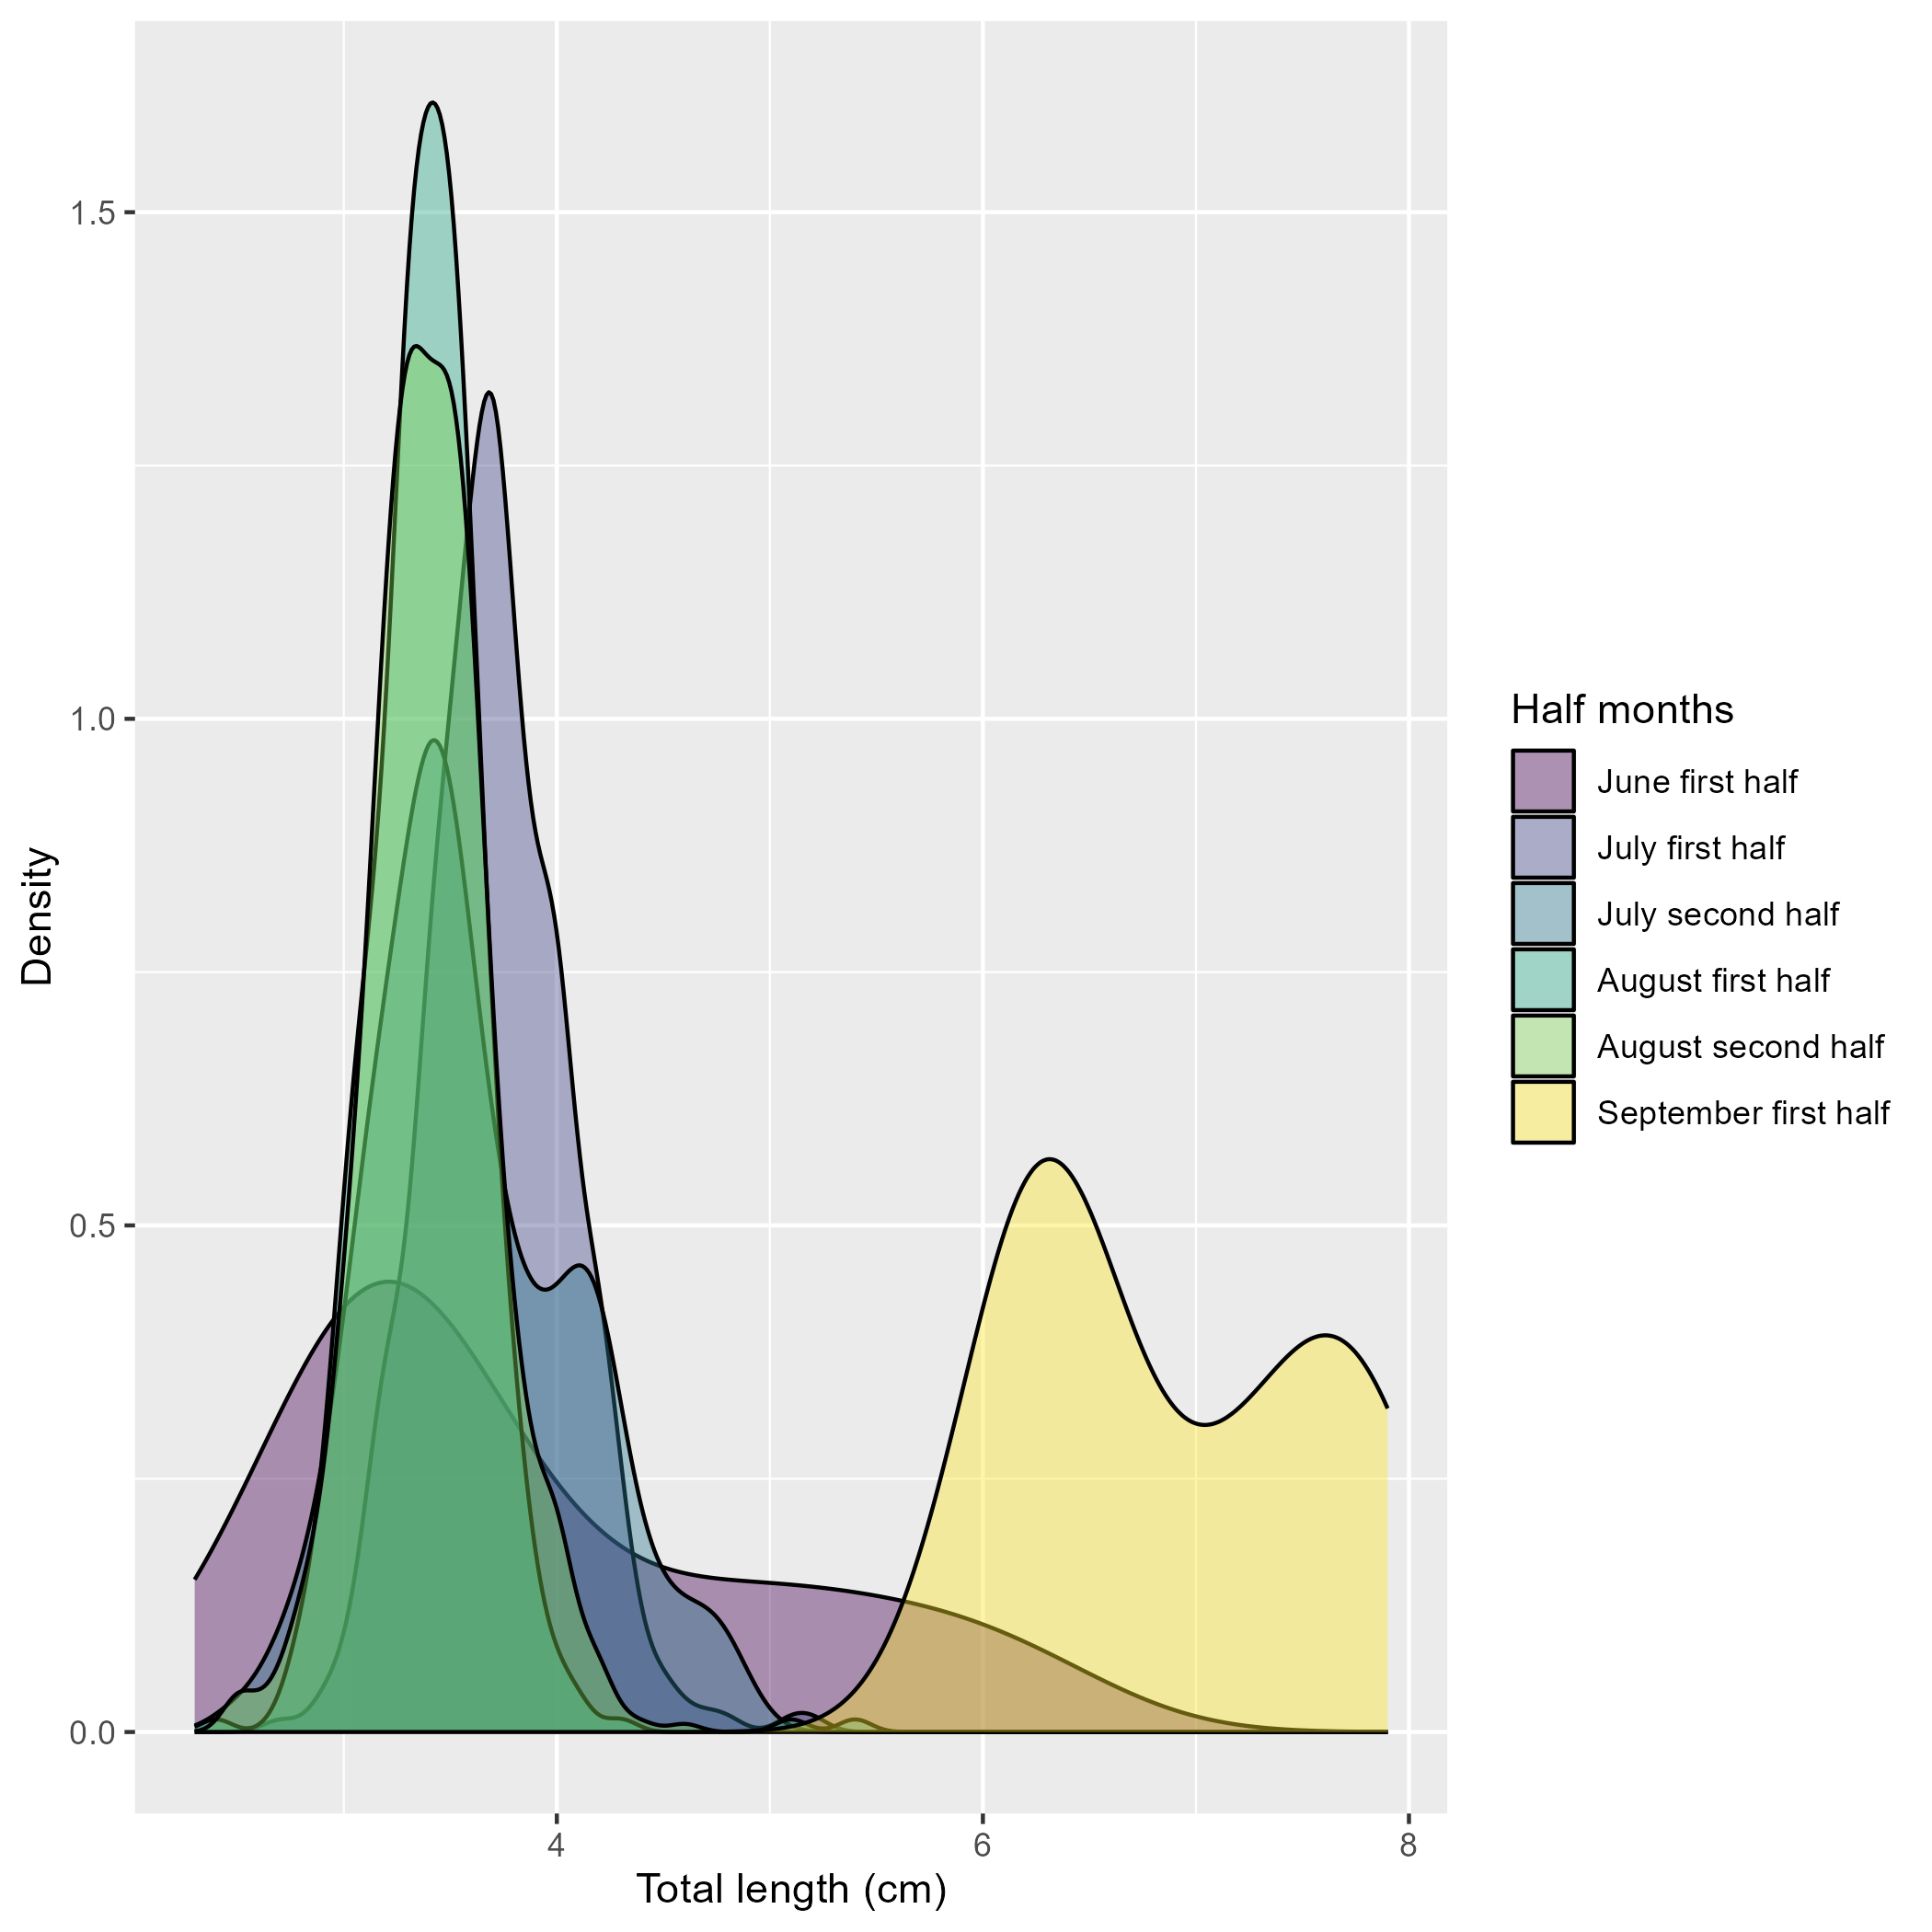
\includegraphics[width=1\textwidth,height=1\textheight]{C:/Users/melissa.monk/Documents/GitHub/copper_rockfish_2023/documents/shared_figures/copper_length_by_half_month.png}
\caption{Distribution of YOY copper rockfish lengths from fish genetically identified from D. Baetscher.\label{fig:copper-smurf-length}}
\end{figure}

\pagebreak

\begin{figure}
\centering
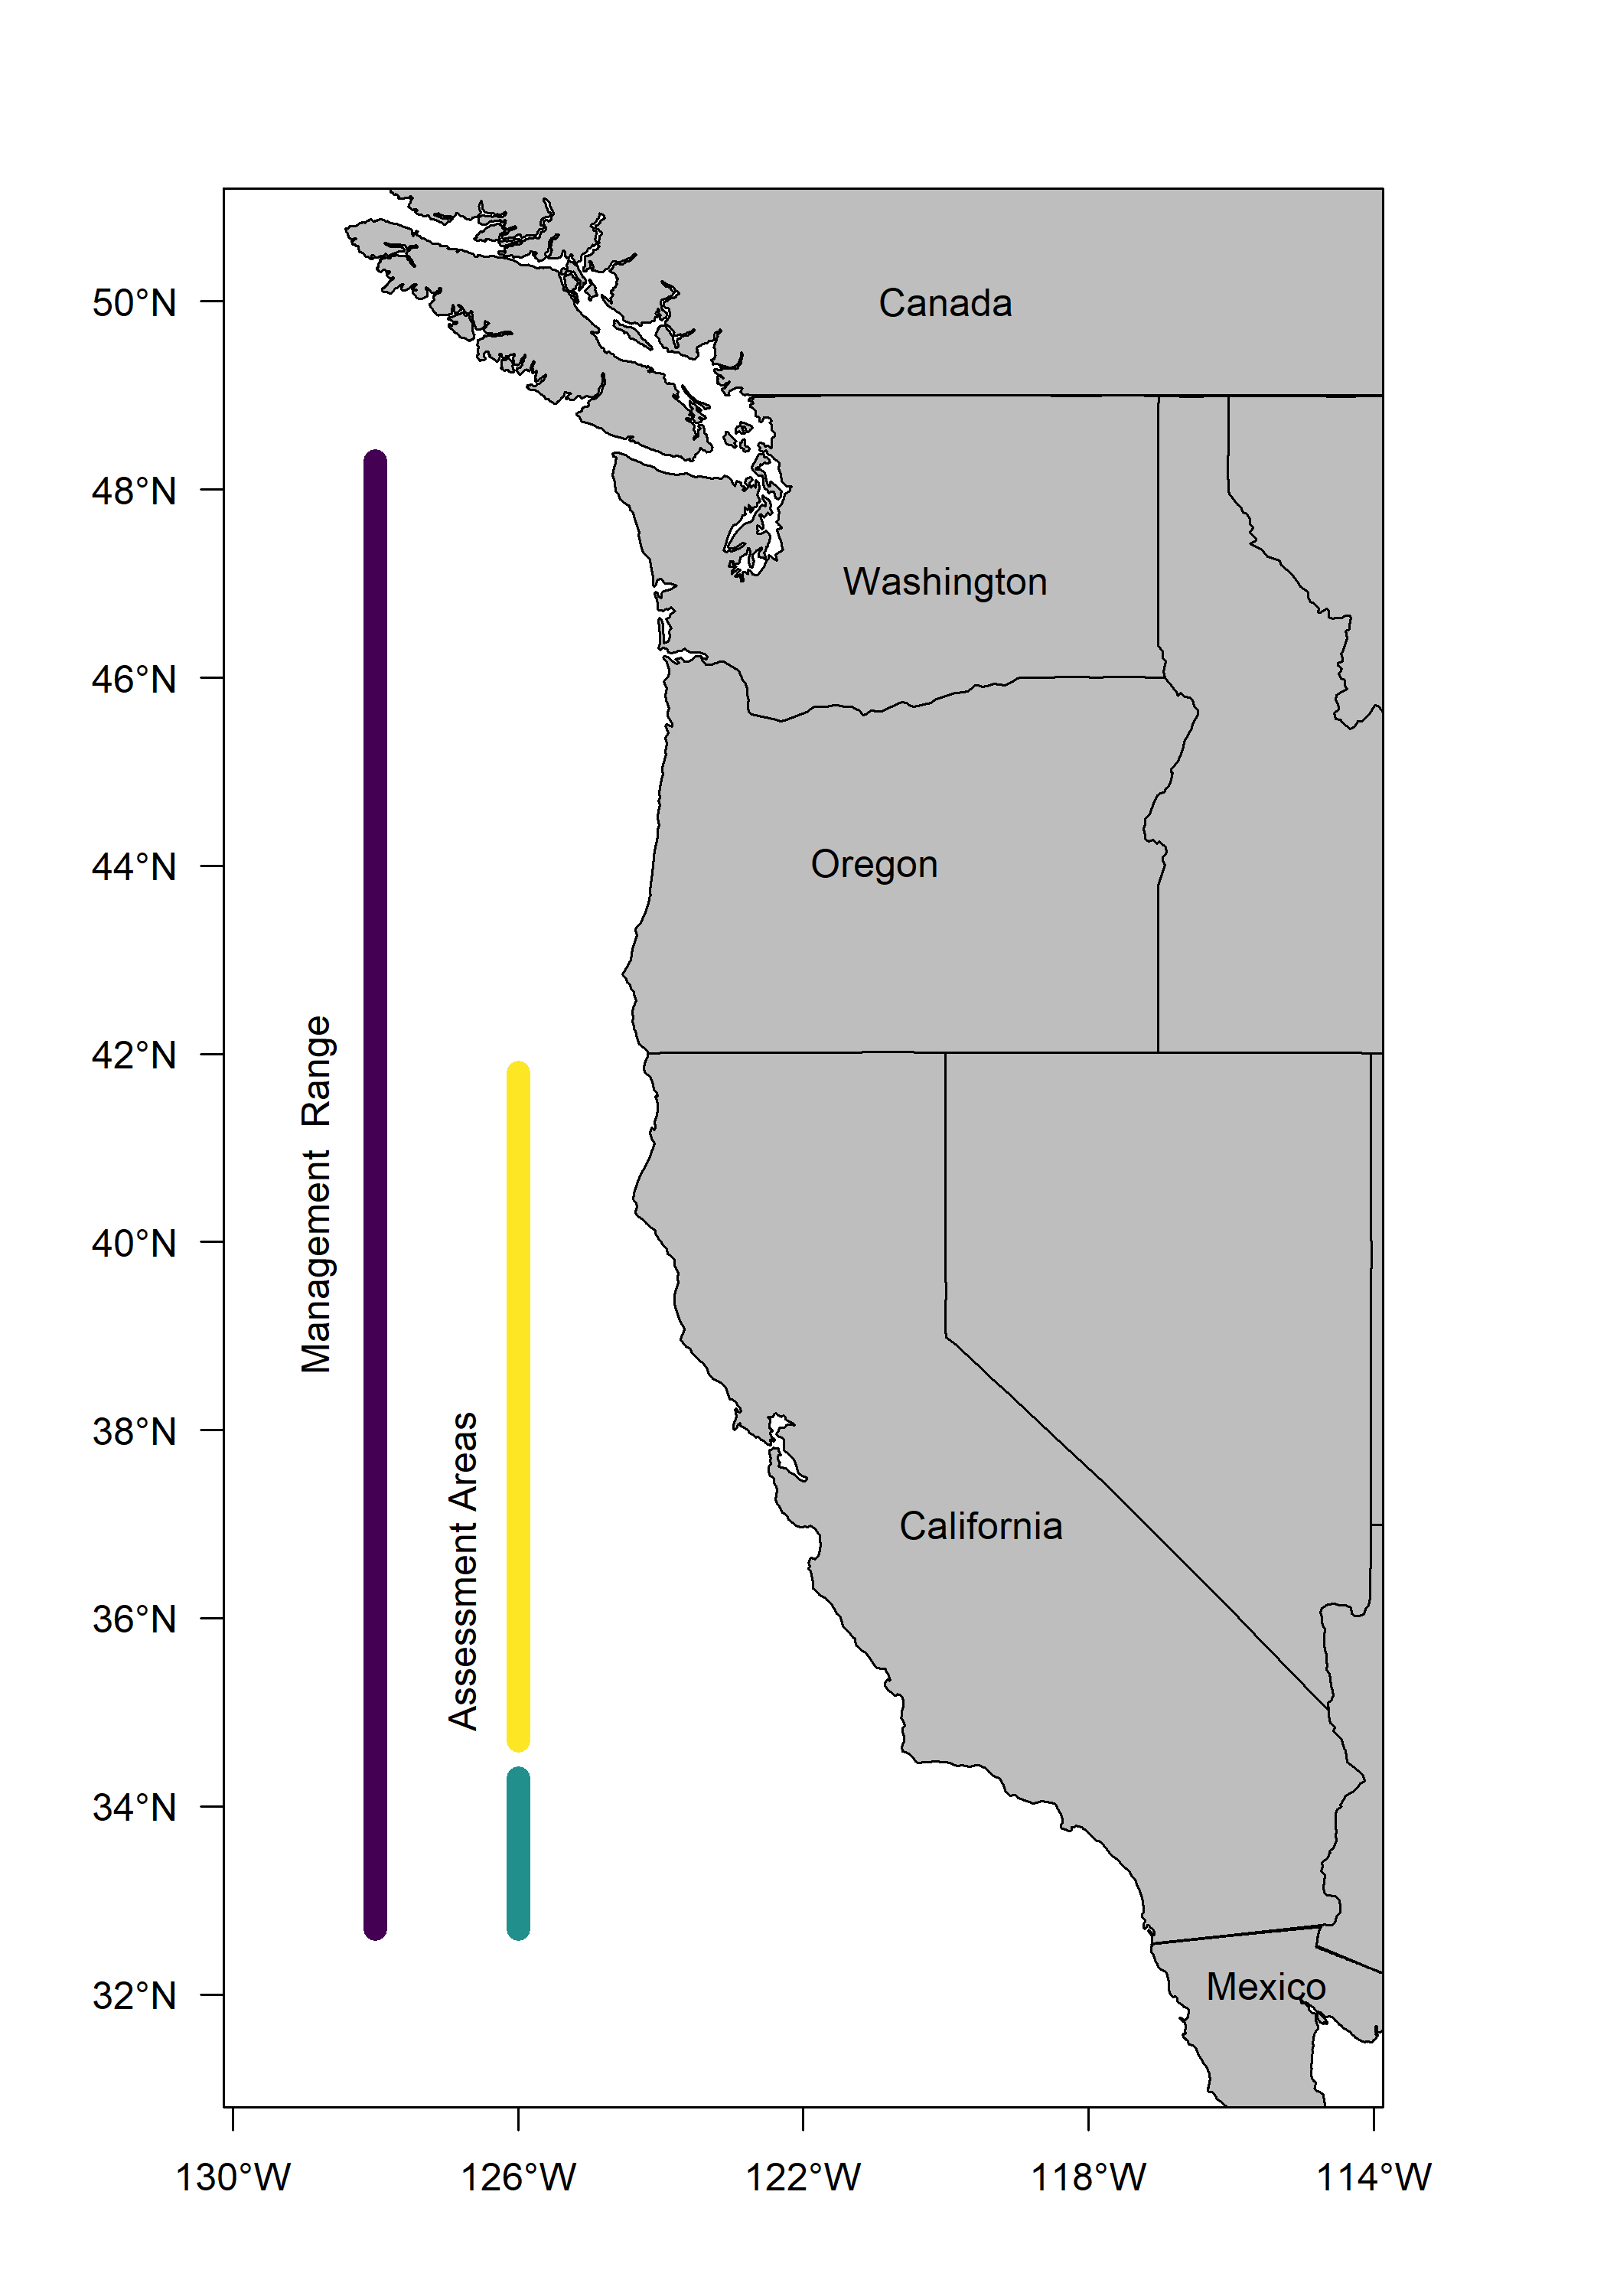
\includegraphics[width=1\textwidth,height=1\textheight]{C:/Users/melissa.monk/Documents/GitHub/copper_rockfish_2023/documents/shared_figures/map.png}
\caption{Map of management area and the 2023 assessments areas for copper rockfish.\label{fig:ca-map}}
\end{figure}

\pagebreak

\begin{figure}
\centering
\includegraphics[width=1\textwidth,height=1\textheight]{S:/copper_rockfish_2023/models/nca/9.8_selex_fix_forecast/plots/catch2 landings stacked.png}
\caption{Landings by fleet used in the base model where catches in metric tons by fleet are stacked.\label{fig:catch}}
\end{figure}

\pagebreak

\begin{figure}
\centering
\includegraphics[width=1\textwidth,height=1\textheight]{S:/copper_rockfish_2023/models/nca/9.8_selex_fix_forecast/plots/data_plot.png}
\caption{Summary of data sources used in the base model.\label{fig:data-plot}}
\end{figure}

\pagebreak

\begin{figure}
\centering
\includegraphics[width=1\textwidth,height=1\textheight]{S:/copper_rockfish_2023/models/nca/9.8_selex_fix_forecast/plots/comp_lendat_bubflt1mkt0.png}
\caption{Length composition data from the commercial dead fleet.\label{fig:com-dead-len-data}}
\end{figure}

\pagebreak

\begin{figure}
\centering
\includegraphics[width=1\textwidth,height=1\textheight]{S:/copper_rockfish_2023/models/nca/9.8_selex_fix_forecast/plots/comp_lendat_data_weighting_TA1.8_Commercial_Dead.png}
\caption{Mean length for commercial dead fleet with 95 percent confidence intervals.\label{fig:mean-com-dead-len-data}}
\end{figure}

\pagebreak

\begin{figure}
\centering
\includegraphics[width=1\textwidth,height=1\textheight]{S:/copper_rockfish_2023/models/nca/9.8_selex_fix_forecast/plots/comp_condAALdat_bubflt1mkt0.png}
\caption{Conditional age-at-length composition data from the commercial dead fleet.\label{fig:com-dead-age-data}}
\end{figure}

\pagebreak

\begin{figure}
\centering
\includegraphics[width=1\textwidth,height=1\textheight]{S:/copper_rockfish_2023/models/nca/9.8_selex_fix_forecast/plots/comp_lendat_bubflt2mkt0.png}
\caption{Length composition data from the commercial live fleet.\label{fig:com-live-len-data}}
\end{figure}

\pagebreak

\begin{figure}
\centering
\includegraphics[width=1\textwidth,height=1\textheight]{S:/copper_rockfish_2023/models/nca/9.8_selex_fix_forecast/plots/comp_lendat_data_weighting_TA1.8_Commercial_Live.png}
\caption{Mean length for commercial live fleet with 95 percent confidence intervals.\label{fig:mean-com-live-len-data}}
\end{figure}

\pagebreak

\begin{figure}
\centering
\includegraphics[width=1\textwidth,height=1\textheight]{S:/copper_rockfish_2023/data/rec_indices/mrfss_cpfv_dockside/north/forSS/Index.png}
\caption{Estimated annual index of abundances for the CPFV fleet based on MRFSS survey data.\label{fig:mrfss-index-main}}
\end{figure}

\pagebreak

\begin{figure}
\centering
\includegraphics[width=1\textwidth,height=1\textheight]{S:/copper_rockfish_2023/data/rec_indices/debwv_cpfv_onboard/deltalogn/Index.png}
\caption{Estimated annual index of abundances for the CPFV fleet based on the Deb Wilson-Vandenberg survey data.\label{fig:dwv-index-main}}
\end{figure}

\pagebreak

\begin{figure}
\centering
\includegraphics[width=1\textwidth,height=1\textheight]{S:/copper_rockfish_2023/data/rec_indices/crfs_cpfv_onboard/north/area_weighted/Index.png}
\caption{Estimated annual index of abundances for the CPFV fleet based on CRFS survey data.\label{fig:crfs-index-main}}
\end{figure}

\pagebreak

\begin{figure}
\centering
\includegraphics[width=1\textwidth,height=1\textheight]{S:/copper_rockfish_2023/data/rec_indices/crfs_pr_dockside/north/rm_last2yrs_area_weighted/Index.png}
\caption{Estimated annual index of abundances for the CPFV fleet based on CRFS survey data.\label{fig:crfs-pr-index-main}}
\end{figure}

\pagebreak

\begin{figure}
\centering
\includegraphics[width=1\textwidth,height=1\textheight]{S:/copper_rockfish_2023/models/nca/9.8_selex_fix_forecast/plots/comp_lendat_bubflt3mkt0_page2.png}
\caption{Length composition data from the recreational CPFV fleet.\label{fig:rec-cpfv-len-data}}
\end{figure}

\pagebreak

\begin{figure}
\centering
\includegraphics[width=1\textwidth,height=1\textheight]{S:/copper_rockfish_2023/models/nca/9.8_selex_fix_forecast/plots/comp_lendat_data_weighting_TA1.8_Rec_CPFV.png}
\caption{Mean length for recreational CPFV fleet with 95 percent confidence intervals.\label{fig:mean-rec-cpfv-len-data}}
\end{figure}

\pagebreak

\begin{figure}
\centering
\includegraphics[width=1\textwidth,height=1\textheight]{S:/copper_rockfish_2023/models/nca/9.8_selex_fix_forecast/plots/comp_condAALdat_bubflt3mkt0.png}
\caption{Conditional age-at-length composition data from the recreational CPFV fleet.\label{fig:rec-cpfv-caal-data}}
\end{figure}

\pagebreak

\begin{figure}
\centering
\includegraphics[width=1\textwidth,height=1\textheight]{S:/copper_rockfish_2023/models/nca/9.8_selex_fix_forecast/plots/comp_agedat_data_weighting_TA1.8_Rec_CPFV.png}
\caption{Mean age for recreational CPFV fleet with 95 percent confidence intervals.\label{fig:mean-rec-cpfv-age-data}}
\end{figure}

\pagebreak

\begin{figure}
\centering
\includegraphics[width=1\textwidth,height=1\textheight]{S:/copper_rockfish_2023/data/ages/plots/coop_crfs_length_comparison.png}
\caption{Comparison of all length collected by the CRFS sampling program for the CPFV fleet to the lengths from the fish with ages from the cooperative sampling program. The length distributions in the area north of Point Conception are in general agreement while the distribution of lengths collected by this program does not align with the length samples from CRFS.\label{fig:coop-len-comparison}}
\end{figure}

\pagebreak

\begin{figure}
\centering
\includegraphics[width=1\textwidth,height=1\textheight]{S:/copper_rockfish_2023/models/nca/9.8_selex_fix_forecast/plots/comp_condAALdat_bubflt4mkt0.png}
\caption{Conditional age-at-length data for recreational PR collected in 2022.\label{fig:rec-pr-caal-data}}
\end{figure}

\pagebreak

\begin{figure}
\centering
\includegraphics[width=1\textwidth,height=1\textheight]{S:/copper_rockfish_2023/models/nca/9.8_selex_fix_forecast/plots/comp_lendat_flt4mkt0_page2.png}
\caption{Length composition data from the recreational PR fleet.\label{fig:rec-pr-len-data}}
\end{figure}

\pagebreak

\begin{figure}
\centering
\includegraphics[width=1\textwidth,height=1\textheight]{S:/copper_rockfish_2023/models/nca/9.8_selex_fix_forecast/plots/comp_lendat_data_weighting_TA1.8_Rec_PR.png}
\caption{Mean length for recreational PR fleet with 95 percent confidence intervals.\label{fig:mean-rec-pr-len-data}}
\end{figure}

\pagebreak

\begin{figure}
\centering
\includegraphics[width=1\textwidth,height=1\textheight]{S:/copper_rockfish_2023/data/survey_indices/plots/north_survey_locations_designation.png}
\caption{Sample locations by each of the fishery-independent data sources used in the base model with indices of abundance, lengths, and ages if collected.\label{fig:survey-locations}}
\end{figure}

\pagebreak

\begin{figure}
\centering
\includegraphics[width=1\textwidth,height=1\textheight]{S:/copper_rockfish_2023/data/survey_indices/plots/north_survey_locations.png}
\caption{Sample locations by area, areas open to fishing (reference) and MPAS, for each of the fishery-independent data sources used in the base model with indices of abundance, lengths, and ages if collected.\label{fig:ref-mpa}}
\end{figure}

\pagebreak

\begin{figure}
\centering
\includegraphics[width=1\textwidth,height=1\textheight]{S:/copper_rockfish_2023/data/survey_indices/ccfrp/north/area_weighted/Index.png}
\caption{Estimated index of abundance from the CCFRP survey.\label{fig:ccfrp-index-main}}
\end{figure}

\pagebreak

\begin{figure}
\centering
\includegraphics[width=1\textwidth,height=1\textheight]{S:/copper_rockfish_2023/models/nca/9.8_selex_fix_forecast/plots/comp_lendat_bubflt5mkt0.png}
\caption{Length composition data from the CCFRP survey.\label{fig:ccfrp-len-data}}
\end{figure}

\pagebreak

\begin{figure}
\centering
\includegraphics[width=1\textwidth,height=1\textheight]{S:/copper_rockfish_2023/models/nca/9.8_selex_fix_forecast/plots/comp_lendat_data_weighting_TA1.8_CCFRP.png}
\caption{Mean length for the CCFRP survey with 95 percent confidence intervals.\label{fig:ccfrp-mean-len-data}}
\end{figure}

\pagebreak

\begin{figure}
\centering
\includegraphics[width=1\textwidth,height=1\textheight]{S:/copper_rockfish_2023/models/nca/9.8_selex_fix_forecast/plots/comp_condAALdat_bubflt5mkt0.png}
\caption{Conditional age-at-length data from the CCFRP survey.\label{fig:ccfrp-age-data}}
\end{figure}

\pagebreak

\begin{figure}
\centering
\includegraphics[width=1\textwidth,height=1\textheight]{S:/copper_rockfish_2023/data/survey_indices/rov/plots/rov_transect_collapsed_copper_north_protection_count.png}
\caption{The location and size of observations across all years and transects.\label{fig:rov-obs-loc}}
\end{figure}

\pagebreak

\begin{figure}
\centering
\includegraphics[width=1\textwidth,height=1\textheight]{S:/copper_rockfish_2023/data/survey_indices/rov/plots/north_raw_cpue_by_mpa_group.png}
\caption{The trend of the calculated CPUE by each MPA and Reference group.\label{fig:rov-raw-cpue}}
\end{figure}

\pagebreak

\begin{figure}
\centering
\includegraphics[width=1\textwidth,height=1\textheight]{S:/copper_rockfish_2023/data/survey_indices/rov/glm_negbin_north_designation_depth/Index.png}
\caption{The estimated weighted relative index of abundance.\label{fig:rov-index-main}}
\end{figure}

\pagebreak

\begin{figure}
\centering
\includegraphics[width=1\textwidth,height=1\textheight]{S:/copper_rockfish_2023/data/survey_indices/rov/plots/rov_length_by_area_designation.png}
\caption{The distribution of lengths across all years for MPA and Reference area north and south of Point Conception.\label{fig:rov-len}}
\end{figure}

\pagebreak

\begin{figure}
\centering
\includegraphics[width=1\textwidth,height=1\textheight]{S:/copper_rockfish_2023/models/nca/9.8_selex_fix_forecast/plots/comp_lendat_flt6mkt0.png}
\caption{Length composition data from the CDFW ROV survey.\label{fig:rov-len-data}}
\end{figure}

\pagebreak

\begin{figure}
\centering
\includegraphics[width=1\textwidth,height=1\textheight]{S:/copper_rockfish_2023/models/nca/9.8_selex_fix_forecast/plots/comp_lendat_data_weighting_TA1.8_CDFW_ROV.png}
\caption{Mean length for CDWF ROV survey with 95 percent confidence intervals.\label{fig:mean-rov-len-data}}
\end{figure}

\pagebreak

\begin{figure}
\centering
\includegraphics[width=1\textwidth,height=1\textheight]{S:/copper_rockfish_2023/data/ages/plots/south_growth_length_comparison.png}
\caption{Length distribution of fish by collection source that were used as conditional age-at-length data in the growth fleet.\label{fig:growth-len-dist}}
\end{figure}

\pagebreak

\begin{figure}
\centering
\includegraphics[width=1\textwidth,height=1\textheight]{S:/copper_rockfish_2023/data/ages/plots/south_growth_age_comparison.png}
\caption{Age distribution of fish by collection source that were used as conditional age-at-length data in the growth fleet.\label{fig:growth-age-dist}}
\end{figure}

\pagebreak

\begin{figure}
\centering
\includegraphics[width=1\textwidth,height=1\textheight]{S:/copper_rockfish_2023/data/wcgbt/north/plots/cpue_map.png}
\caption{Location and catch-per-unit-effort by location caught north of Point Conception by the NWFSC WCGBT survey.\label{fig:wcgbt-cpue}}
\end{figure}

\pagebreak

\begin{figure}
\centering
\includegraphics[width=1\textwidth,height=1\textheight]{S:/copper_rockfish_2023/data/wcgbt/north/plots/presence-absence_proportion_by_depth.png}
\caption{Number of positive tows across all years by depth in meters.\label{fig:wcgbt-depth}}
\end{figure}

\pagebreak

\begin{figure}
\centering
\includegraphics[width=1\textwidth,height=1\textheight]{S:/copper_rockfish_2023/data/wcgbt/plots/wcgbt_north_age_at_length_by_area.png}
\caption{Age and length by sex for copper rockfish caught north of Point Conception by the NWFSC WCGBT survey.\label{fig:wcgbt-len-age}}
\end{figure}

\pagebreak

\hypertarget{biology}{%
\subsection{Biology}\label{biology}}

\begin{figure}
\centering
\includegraphics[width=1\textwidth,height=1\textheight]{S:/copper_rockfish_2023/models/nca/9.8_selex_fix_forecast/plots/bio6_maturity.png}
\caption{Maturity as a function of length.\label{fig:maturity}}
\end{figure}

\pagebreak

\begin{figure}
\centering
\includegraphics[width=1\textwidth,height=1\textheight]{S:/copper_rockfish_2023/models/nca/9.8_selex_fix_forecast/plots/bio9_fecundity_len.png}
\caption{Fecundity as a function of length.\label{fig:fecundity}}
\end{figure}

\pagebreak

\begin{figure}
\centering
\includegraphics[width=1\textwidth,height=1\textheight]{S:/copper_rockfish_2023/data/wcgbt/plots/length_fraction_female.png}
\caption{Fraction of each sex by length by the NWFSC WCGBT survey.\label{fig:frac-sex-len}}
\end{figure}

\pagebreak

\begin{figure}
\centering
\includegraphics[width=1\textwidth,height=1\textheight]{S:/copper_rockfish_2023/data/biology/plots/Length_Weight_All.png}
\caption{Estimated weight-at-length.\label{fig:est-len-wght}}
\end{figure}

\pagebreak

\begin{figure}
\centering
\includegraphics[width=1\textwidth,height=1\textheight]{S:/copper_rockfish_2023/data/ages/ageing_error/B0_S3/Reader_1_vs_Reader_2.png}
\caption{Distribution of double reads between age reader 1 and 2.\label{fig:age-error-dist}}
\end{figure}

\pagebreak

\begin{figure}
\centering
\includegraphics[width=1\textwidth,height=1\textheight]{S:/copper_rockfish_2023/models/nca/9.8_selex_fix_forecast/plots/numbers5_ageerrorSD.png}
\caption{Ageing imprecision standard deviation of observed age in years.\label{fig:age-error}}
\end{figure}

\pagebreak

\begin{figure}
\centering
\includegraphics[width=1\textwidth,height=1\textheight]{S:/copper_rockfish_2023/models/nca/9.8_selex_fix_forecast/plots/numbers10_ageerror_matrix_1.png}
\caption{Distribution of observed age at true age for ageing error type 1.\label{fig:age-error-matrix}}
\end{figure}

\pagebreak

\hypertarget{model-results}{%
\subsection{Model Results}\label{model-results}}

\hypertarget{model-bridging}{%
\subsubsection{Model Bridging}\label{model-bridging}}

\begin{figure}
\centering
\includegraphics[width=1\textwidth,height=1\textheight]{S:/copper_rockfish_2023/models/nca/_bridging/_plots/0_model_convert_compare2_spawnbio_uncertainty.png}
\caption{Model version bridge comparison of estimated spawning output.\label{fig:bridge-ssb}}
\end{figure}

\pagebreak

\begin{figure}
\centering
\includegraphics[width=1\textwidth,height=1\textheight]{S:/copper_rockfish_2023/models/nca/_bridging/_plots/0_model_convert_compare4_Bratio_uncertainty.png}
\caption{Model version bridge comparison of estimated fraction unfished.\label{fig:bridge-depl}}
\end{figure}

\pagebreak

\begin{figure}
\centering
\includegraphics[width=1\textwidth,height=1\textheight]{S:/copper_rockfish_2023/models/nca/_bridging/_plots/full_bridge_1_compare2_spawnbio_uncertainty.png}
\caption{Model structure and data bridging comparison of estimated spawning output.\label{fig:data-bridge-ssb-1}}
\end{figure}

\pagebreak

\begin{figure}
\centering
\includegraphics[width=1\textwidth,height=1\textheight]{S:/copper_rockfish_2023/models/nca/_bridging/_plots/full_bridge_1_compare4_Bratio_uncertainty.png}
\caption{Model structure and data bridging comparison of estimated fraction unfished.\label{fig:data-bridge-depl-1}}
\end{figure}

\pagebreak

\begin{figure}
\centering
\includegraphics[width=1\textwidth,height=1\textheight]{S:/copper_rockfish_2023/models/nca/_bridging/_plots/full_bridge_2_compare2_spawnbio_uncertainty.png}
\caption{Model structure and data bridging comparison of estimated spawning output.\label{fig:data-bridge-ssb-2}}
\end{figure}

\pagebreak

\begin{figure}
\centering
\includegraphics[width=1\textwidth,height=1\textheight]{S:/copper_rockfish_2023/models/nca/_bridging/_plots/full_bridge_2_compare4_Bratio_uncertainty.png}
\caption{Model structure and data bridging comparison of estimated fraction unfished.\label{fig:data-bridge-depl-2}}
\end{figure}

\pagebreak

\pagebreak

\hypertarget{biology-1}{%
\subsubsection{Biology}\label{biology-1}}

\begin{figure}
\centering
\includegraphics[width=1\textwidth,height=1\textheight]{S:/copper_rockfish_2023/models/nca/9.8_selex_fix_forecast/plots/bio1_sizeatage.png}
\caption{Model estimated length-at-age in the beginning of the year. Shaded area indicates 95 percent distribution of length-at-age around the estimated growth curve.\label{fig:mod-est-len-age}}
\end{figure}

\pagebreak

\hypertarget{selectivity}{%
\subsubsection{Selectivity}\label{selectivity}}

\begin{figure}
\centering
\includegraphics[width=1\textwidth,height=1\textheight]{S:/copper_rockfish_2023/models/nca/9.8_selex_fix_forecast/plots/north_selectivity.png}
\caption{Estimated selectivity for each fleet and survey in the base model.\label{fig:est-selex}}
\end{figure}

\pagebreak

\hypertarget{recruitment}{%
\subsubsection{Recruitment}\label{recruitment}}

\begin{figure}
\centering
\includegraphics[width=1\textwidth,height=1\textheight]{S:/copper_rockfish_2023/models/nca/9.8_selex_fix_forecast/plots/ts11_Age-0_recruits_(1000s)_with_95_asymptotic_intervals.png}
\caption{Estimated time series of age-0 recruits (1000s).\label{fig:recruits}}
\end{figure}

\pagebreak

\begin{figure}
\centering
\includegraphics[width=1\textwidth,height=1\textheight]{S:/copper_rockfish_2023/models/nca/9.8_selex_fix_forecast/plots/recdevs2_withbars.png}
\caption{Estimated time series of recruitment deviations.\label{fig:rec-devs}}
\end{figure}

\pagebreak

\begin{figure}
\centering
\includegraphics[width=1\textwidth,height=1\textheight]{S:/copper_rockfish_2023/models/nca/9.8_selex_fix_forecast/plots/recruit_fit_bias_adjust.png}
\caption{Points are transformed variances. Red line shows current settings for bias adjustment specified in control file. Blue line shows least squares estimate of alternative bias adjustment relationship for recruitment deviations (which may or may not be an improvement).\label{fig:bias-adjust}}
\end{figure}

\newpage

\begin{figure}
\centering
\includegraphics[width=1\textwidth,height=1\textheight]{S:/copper_rockfish_2023/models/nca/9.8_selex_fix_forecast/plots/SR_curve.png}
\caption{Stock-recruit curve. Point colors indicate year, with warmer colors indicating earlier years and cooler colors in showing later years.\label{fig:bh-curve}}
\end{figure}

\pagebreak

\hypertarget{fits-to-data}{%
\subsubsection{Fits to Data}\label{fits-to-data}}

\begin{figure}
\centering
\includegraphics[width=1\textwidth,height=1\textheight]{S:/copper_rockfish_2023/models/nca/9.8_selex_fix_forecast/plots/comp_lenfit__aggregated_across_time.png}
\caption{Length composition aggregated across years by fleet with the model estimated fit to the data by sex (green unsexed, red female, and blue male).\label{fig:len-agg-fit}}
\end{figure}

\pagebreak

\begin{figure}
\centering
\includegraphics[width=1\textwidth,height=1\textheight]{S:/copper_rockfish_2023/models/nca/9.8_selex_fix_forecast/plots/comp_lenfit_residsflt1mkt0.png}
\caption{Pearson residuals for commercial fleet. Closed bubble are positive residuals (observed \textgreater{} expected) and open bubbles are negative residuals (observed \textless{} expected).\label{fig:com-dead-pearson}}
\end{figure}

\pagebreak

\begin{figure}
\centering
\includegraphics[width=1\textwidth,height=1\textheight]{S:/copper_rockfish_2023/models/nca/9.8_selex_fix_forecast/plots/comp_lenfit_data_weighting_TA1.8_Commercial_dead.png}
\caption{Mean length for commercial dead lengths with 95 percent confidence intervals based on current samples sizes.\label{fig:com-dead-mean-len-fit}}
\end{figure}

\pagebreak

\pagebreak

\begin{figure}
\centering
\includegraphics[width=1\textwidth,height=1\textheight]{S:/copper_rockfish_2023/models/nca/9.8_selex_fix_forecast/plots/comp_lenfit_residsflt2mkt0.png}
\caption{Pearson residuals for commercial live fleet. Closed bubble are positive residuals (observed \textgreater{} expected) and open bubbles are negative residuals (observed \textless{} expected).\label{fig:com-live-pearson}}
\end{figure}

\pagebreak

\begin{figure}
\centering
\includegraphics[width=1\textwidth,height=1\textheight]{S:/copper_rockfish_2023/models/nca/9.8_selex_fix_forecast/plots/comp_lenfit_data_weighting_TA1.8_Commercial_live.png}
\caption{Mean length for commercial live fish lengths with 95 percent confidence intervals based on current samples sizes.\label{fig:com-live-mean-len-fit}}
\end{figure}

\pagebreak

\begin{figure}
\centering
\includegraphics[width=1\textwidth,height=1\textheight]{S:/copper_rockfish_2023/models/nca/9.8_selex_fix_forecast/plots/comp_lenfit_residsflt3mkt0_page2.png}
\caption{Pearson residuals for recreational CPFV fleet. Closed bubble are positive residuals (observed \textgreater{} expected) and open bubbles are negative residuals (observed \textless{} expected).\label{fig:rec-cpfv-pearson}}
\end{figure}

\pagebreak

\begin{figure}
\centering
\includegraphics[width=1\textwidth,height=1\textheight]{S:/copper_rockfish_2023/models/nca/9.8_selex_fix_forecast/plots/comp_lenfit_data_weighting_TA1.8_Rec_CPFV.png}
\caption{Mean length for recreational CPFV lengths with 95 percent confidence intervals based on current samples sizes.\label{fig:rec-cpfv-mean-len-fit}}
\end{figure}

\pagebreak

\begin{figure}
\centering
\includegraphics[width=1\textwidth,height=1\textheight]{S:/copper_rockfish_2023/models/nca/9.8_selex_fix_forecast/plots/comp_agefit_residsflt3mkt0.png}
\caption{Pearson residuals for recreational CPFV age data. Closed bubble are positive residuals (observed \textgreater{} expected) and open bubbles are negative residuals (observed \textless{} expected).\label{fig:rec-cpfv-age-pearson}}
\end{figure}

\pagebreak

\begin{figure}
\centering
\includegraphics[width=1\textwidth,height=1\textheight]{S:/copper_rockfish_2023/models/nca/9.8_selex_fix_forecast/plots/comp_lenfit_residsflt4mkt0_page2.png}
\caption{Pearson residuals for recreational private/rental fleet. Closed bubble are positive residuals (observed \textgreater{} expected) and open bubbles are negative residuals (observed \textless{} expected).\label{fig:rec-pr-pearson}}
\end{figure}

\pagebreak

\begin{figure}
\centering
\includegraphics[width=1\textwidth,height=1\textheight]{S:/copper_rockfish_2023/models/nca/9.8_selex_fix_forecast/plots/comp_lenfit_data_weighting_TA1.8_Rec_PR.png}
\caption{Mean length for recreational private/rental lengths with 95 percent confidence intervals based on current samples sizes.\label{fig:rec-pr-mean-len-fit}}
\end{figure}

\pagebreak

\begin{figure}
\centering
\includegraphics[width=1\textwidth,height=1\textheight]{S:/copper_rockfish_2023/models/nca/9.8_selex_fix_forecast/plots/comp_lenfit_residsflt5mkt0.png}
\caption{Pearson residuals for CCFRP Hook and Line survey length data. Closed bubble are positive residuals (observed \textgreater{} expected) and open bubbles are negative residuals (observed \textless{} expected).\label{fig:ccfrp-len-pearson}}
\end{figure}

\pagebreak

\begin{figure}
\centering
\includegraphics[width=1\textwidth,height=1\textheight]{S:/copper_rockfish_2023/models/nca/9.8_selex_fix_forecast/plots/comp_lenfit_data_weighting_TA1.8_CCFRP.png}
\caption{Mean length for CCFRP Hook and Line survey lengths with 95 percent confidence intervals based on current samples sizes.\label{fig:ccfrp-mean-len-fit}}
\end{figure}

\pagebreak

\begin{figure}
\centering
\includegraphics[width=1\textwidth,height=1\textheight]{S:/copper_rockfish_2023/models/nca/9.8_selex_fix_forecast/plots/comp_condAAlfit_residsflt5mkt0.png}
\caption{Pearson residuals for CCFRP Hook and Line survey conditional-age-at-length data. Closed bubble are positive residuals (observed \textgreater{} expected) and open bubbles are negative residuals (observed \textless{} expected).\label{fig:ccfrp-age-pearson}}
\end{figure}

\pagebreak

\begin{figure}
\centering
\includegraphics[width=1\textwidth,height=1\textheight]{S:/copper_rockfish_2023/models/nca/9.8_selex_fix_forecast/plots/comp_lenfit_residsflt6mkt0.png}
\caption{Pearson residuals for CDFW ROV survey length data. Closed bubble are positive residuals (observed \textgreater{} expected) and open bubbles are negative residuals (observed \textless{} expected).\label{fig:rov-pearson}}
\end{figure}

\pagebreak

\begin{figure}
\centering
\includegraphics[width=1\textwidth,height=1\textheight]{S:/copper_rockfish_2023/models/nca/9.8_selex_fix_forecast/plots/comp_lenfit_data_weighting_TA1.8_CDFW_ROV.png}
\caption{Mean length for CDFW ROV survey lengths with 95 percent confidence intervals based on current samples sizes.\label{fig:rov-mean-len-fit}}
\end{figure}

\pagebreak

\begin{figure}
\centering
\includegraphics[width=1\textwidth,height=1\textheight]{S:/copper_rockfish_2023/models/nca/9.8_selex_fix_forecast/plots/index5_logcpuefit_Rec_CPFV.png}
\caption{Fit to log index data on log scale for recreational (MRFSS) CPFV. Lines indicate 95\% uncertainty interval around index values based on the model assumption of lognormal error. Thicker lines (if present) indicate input uncertainty before addition of estimated additional uncertainty parameter.\label{fig:mrfss-cpfv-index-fit}}
\end{figure}

\pagebreak

\begin{figure}
\centering
\includegraphics[width=1\textwidth,height=1\textheight]{S:/copper_rockfish_2023/models/nca/9.8_selex_fix_forecast/plots/index5_logcpuefit_DWV_CPFV.png}
\caption{Fit to log index data on log scale for Deb Wilson-Vandenberg CPFV survey. Lines indicate 95\% uncertainty interval around index values based on the model assumption of lognormal error. Thicker lines (if present) indicate input uncertainty before addition of estimated additional uncertainty parameter.\label{fig:dwv-cpfv-index-fit}}
\end{figure}

\pagebreak

\begin{figure}
\centering
\includegraphics[width=1\textwidth,height=1\textheight]{S:/copper_rockfish_2023/models/nca/9.8_selex_fix_forecast/plots/index5_logcpuefit_CRFS_CPFV.png}
\caption{Fit to log index data on log scale for CRFS CPFV survey. Lines indicate 95\% uncertainty interval around index values based on the model assumption of lognormal error. Thicker lines (if present) indicate input uncertainty before addition of estimated additional uncertainty parameter.\label{fig:crfs-cpfv-index-fit}}
\end{figure}

\pagebreak

\begin{figure}
\centering
\includegraphics[width=1\textwidth,height=1\textheight]{S:/copper_rockfish_2023/models/nca/9.8_selex_fix_forecast/plots/index5_logcpuefit_Rec_PR.png}
\caption{Fit to log index data on log scale for recreational (CRFS) PR. Lines indicate 95\% uncertainty interval around index values based on the model assumption of lognormal error. Thicker lines (if present) indicate input uncertainty before addition of estimated additional uncertainty parameter.\label{fig:crfs-pr-index-fit}}
\end{figure}

\pagebreak

\begin{figure}
\centering
\includegraphics[width=1\textwidth,height=1\textheight]{S:/copper_rockfish_2023/models/nca/9.8_selex_fix_forecast/plots/index5_logcpuefit_CCFRP.png}
\caption{Fit to log index data on log scale for CCFRP survey. Lines indicate 95\% uncertainty interval around index values based on the model assumption of lognormal error. Thicker lines (if present) indicate input uncertainty before addition of estimated additional uncertainty parameter.\label{fig:ccfrp-index-fit}}
\end{figure}

\pagebreak

\begin{figure}
\centering
\includegraphics[width=1\textwidth,height=1\textheight]{S:/copper_rockfish_2023/models/nca/9.8_selex_fix_forecast/plots/index5_logcpuefit_CDFW_ROV.png}
\caption{Fit to log index data on log scale for CDFW ROV survey. Lines indicate 95\% uncertainty interval around index values based on the model assumption of lognormal error. Thicker lines (if present) indicate input uncertainty before addition of estimated additional uncertainty parameter.\label{fig:rov-index-fit}}
\end{figure}

\pagebreak

\begin{figure}
\centering
\includegraphics[width=1\textwidth,height=1\textheight]{S:/copper_rockfish_2023/models/nca/9.8_selex_fix_forecast/plots/index9_standcpueall.png}
\caption{Standardized indices overlaid. Each index is rescaled to have mean observation = 1.0.\label{fig:standardized-indices}}
\end{figure}

\pagebreak

\hypertarget{time-series}{%
\subsubsection{Time-series}\label{time-series}}

\begin{figure}
\centering
\includegraphics[width=1\textwidth,height=1\textheight]{S:/copper_rockfish_2023/models/nca/9.8_selex_fix_forecast/plots/ts7_Spawning_output_with_95_asymptotic_intervals_intervals.png}
\caption{Estimated time series of spawning biomass.\label{fig:ssb}}
\end{figure}

\pagebreak

\begin{figure}
\centering
\includegraphics[width=1\textwidth,height=1\textheight]{S:/copper_rockfish_2023/models/nca/9.8_selex_fix_forecast/plots/ts1_Total_biomass_(mt).png}
\caption{Estimated time series of total biomass.\label{fig:tot-bio}}
\end{figure}

\pagebreak

\begin{figure}
\centering
\includegraphics[width=1\textwidth,height=1\textheight]{S:/copper_rockfish_2023/models/nca/9.8_selex_fix_forecast/plots/ts9_Relative_spawning_output_intervals.png}
\caption{Estimated time series of fraction of unfished spawning biomass.\label{fig:depl}}
\end{figure}

\pagebreak

\begin{figure}
\centering
\includegraphics[width=1\textwidth,height=1\textheight]{C:/Users/melissa.monk/Documents/GitHub/copper_rockfish_2023/documents/shared_figures/spawning_output_combined.png}
\caption{Estimated combined time series of spawning output for copper rockfish in California waters.\label{fig:sb-all}}
\end{figure}

\clearpage

\begin{figure}
\centering
\includegraphics[width=1\textwidth,height=1\textheight]{C:/Users/melissa.monk/Documents/GitHub/copper_rockfish_2023/documents/shared_figures/depletion_combined.png}
\caption{Estimated combined time series of fraction of relative spawning output for copper rockfish in California waters.\label{fig:depl-all}}
\end{figure}

\clearpage

\hypertarget{sensitivity-analyses-and-retrospectives}{%
\subsubsection{Sensitivity Analyses and Retrospectives}\label{sensitivity-analyses-and-retrospectives}}

\begin{figure}
\centering
\includegraphics[width=1\textwidth,height=1\textheight]{S:/copper_rockfish_2023/models/nca/_sensitivities/_plots/Sensi_REplot_all_horizontal.png}
\caption{Comparison of the relative change in estimated management quantities as compared to the base model. The quantities compared are the estimate of unfished spawning biomass (SB0), spawning output in 2023 (SB2023), the relative spawnin output (SB2023/SB0), the yield based on a spawner per recruit harvest rate (YieldSPR=0.50), and the fishing mortality at that harvest rate (FSPR=0.50). The colored boxes indicate the 95 percent confidence interval around the point estimate of the quantity from the base model where each color corresponds with a specific quantity in the legend. A model with matching estimates as the base model would reflect a relative change of 0, a model with estimates less than the base model would have a negative relative change, and a model with estimates greater than the base model would have a positive relative change.\label{fig:sens-all}}
\end{figure}

\newpage

\begin{figure}
\centering
\includegraphics[width=1\textwidth,height=1\textheight]{S:/copper_rockfish_2023/models/nca/_sensitivities/_plots/9.8_selex_fix_forecast_final_1_compare2_spawnbio_uncertainty.png}
\caption{Change in estimated spawning output by sensitivity.\label{fig:sens-ssb-1}}
\end{figure}

\newpage

\begin{figure}
\centering
\includegraphics[width=1\textwidth,height=1\textheight]{S:/copper_rockfish_2023/models/nca/_sensitivities/_plots/9.8_selex_fix_forecast_final_1_compare4_Bratio_uncertainty.png}
\caption{Change in estimated fraction unfished by sensitivity.\label{fig:sens-depl-1}}
\end{figure}

\newpage

\begin{figure}
\centering
\includegraphics[width=1\textwidth,height=1\textheight]{S:/copper_rockfish_2023/models/nca/_sensitivities/_plots/9.8_selex_fix_forecast_final_2_compare2_spawnbio_uncertainty.png}
\caption{Change in estimated spawning output by sensitivity.\label{fig:sens-ssb-2}}
\end{figure}

\newpage

\begin{figure}
\centering
\includegraphics[width=1\textwidth,height=1\textheight]{S:/copper_rockfish_2023/models/nca/_sensitivities/_plots/9.8_selex_fix_forecast_final_2_compare4_Bratio_uncertainty.png}
\caption{Change in estimated fraction unfished by sensitivity.\label{fig:sens-depl-2}}
\end{figure}

\newpage

\begin{figure}
\centering
\includegraphics[width=1\textwidth,height=1\textheight]{S:/copper_rockfish_2023/models/nca/_sensitivities/_plots/9.8_selex_fix_forecast_final_3_compare2_spawnbio_uncertainty.png}
\caption{Change in estimated spawning output by sensitivity.\label{fig:sens-ssb-3}}
\end{figure}

\newpage

\begin{figure}
\centering
\includegraphics[width=1\textwidth,height=1\textheight]{S:/copper_rockfish_2023/models/nca/_sensitivities/_plots/9.8_selex_fix_forecast_final_3_compare4_Bratio_uncertainty.png}
\caption{Change in estimated fraction unfished by sensitivity.\label{fig:sens-depl-3}}
\end{figure}

\newpage

\begin{figure}
\centering
\includegraphics[width=1\textwidth,height=1\textheight]{N:/Assessments/CurrentAssessments/copper_rockfish_2023/models/nca/9.8_selex_fix_forecast_retro/compare2_spawnbio_uncertainty.png}
\caption{Change in the estimate of spawning output when the most recent 5 years of data area removed sequentially.\label{fig:retro-ssb}}
\end{figure}

\pagebreak

\begin{figure}
\centering
\includegraphics[width=1\textwidth,height=1\textheight]{N:/Assessments/CurrentAssessments/copper_rockfish_2023/models/nca/9.8_selex_fix_forecast_retro/compare4_Bratio_uncertainty.png}
\caption{Change in the estimate of fraction unfished when the most recent 5 years of data area removed sequentially.\label{fig:retro-depl}}
\end{figure}

\pagebreak

\hypertarget{likelihood-profiles}{%
\subsubsection{Likelihood Profiles}\label{likelihood-profiles}}

\begin{figure}
\centering
\includegraphics[width=1\textwidth,height=1\textheight]{S:/copper_rockfish_2023/models/nca/9.8_selex_fix_forecast_profile_SR_LN(R0)_prior_like_0/piner_panel_SR_LN(R0).png}
\caption{Change in the negative log-likelihood across a range of log(R\textsubscript{0}) values.\label{fig:r0-profile}}
\end{figure}

\pagebreak

\begin{figure}
\centering
\includegraphics[width=1\textwidth,height=1\textheight]{S:/copper_rockfish_2023/models/nca/9.8_selex_fix_forecast_profile_SR_LN(R0)_prior_like_0/SR_LN(R0)_trajectories_compare1_spawnbio.png}
\caption{Change in the estimate of spawning output across a range of log(R\textsubscript{0}) values.\label{fig:r0-ssb}}
\end{figure}

\pagebreak

\begin{figure}
\centering
\includegraphics[width=1\textwidth,height=1\textheight]{S:/copper_rockfish_2023/models/nca/9.8_selex_fix_forecast_profile_SR_LN(R0)_prior_like_0/SR_LN(R0)_trajectories_compare3_Bratio.png}
\caption{Change in the estimate of fraction unfished across a range of log(R\textsubscript{0}) values.\label{fig:r0-depl}}
\end{figure}

\pagebreak

\begin{figure}
\centering
\includegraphics[width=1\textwidth,height=1\textheight]{S:/copper_rockfish_2023/models/nca/9.8_selex_fix_forecast_profile_SR_BH_steep_prior_like_1/piner_panel_SR_BH_steep.png}
\caption{Change in the negative log-likelihood across a range of steepness values.\label{fig:h-profile}}
\end{figure}

\pagebreak

\begin{figure}
\centering
\includegraphics[width=1\textwidth,height=1\textheight]{S:/copper_rockfish_2023/models/nca/9.8_selex_fix_forecast_profile_SR_BH_steep_prior_like_1/SR_BH_steep_trajectories_compare1_spawnbio.png}
\caption{Change in the estimate of spawning output across a range of steepness values.\label{fig:h-ssb}}
\end{figure}

\pagebreak

\begin{figure}
\centering
\includegraphics[width=1\textwidth,height=1\textheight]{S:/copper_rockfish_2023/models/nca/9.8_selex_fix_forecast_profile_SR_BH_steep_prior_like_1/SR_BH_steep_trajectories_compare3_Bratio.png}
\caption{Change in the estimate of fraction unfished across a range of steepness values.\label{fig:h-depl}}
\end{figure}

\pagebreak

\begin{figure}
\centering
\includegraphics[width=1\textwidth,height=1\textheight]{S:/copper_rockfish_2023/models/nca/9.8_selex_fix_forecast_profile_NatM_uniform_Fem_GP_1_prior_like_1/piner_panel_NatM_uniform_Fem_GP_1.png}
\caption{Change in the negative log-likelihood across a range of female natural mortality values.\label{fig:m-profile}}
\end{figure}

\pagebreak

\begin{figure}
\centering
\includegraphics[width=1\textwidth,height=1\textheight]{S:/copper_rockfish_2023/models/nca/9.8_selex_fix_forecast_profile_NatM_uniform_Fem_GP_1_prior_like_1/NatM_uniform_Fem_GP_1_trajectories_compare1_spawnbio.png}
\caption{Change in the estimate of spawning output across a range of female natural mortality values.\label{fig:m-ssb}}
\end{figure}

\pagebreak

\begin{figure}
\centering
\includegraphics[width=1\textwidth,height=1\textheight]{S:/copper_rockfish_2023/models/nca/9.8_selex_fix_forecast_profile_NatM_uniform_Fem_GP_1_prior_like_1/NatM_uniform_Fem_GP_1_trajectories_compare3_Bratio.png}
\caption{Change in the estimate of fraction unfished across a range of female natural values.\label{fig:m-depl}}
\end{figure}

\begin{figure}
\centering
\includegraphics[width=1\textwidth,height=1\textheight]{C:/Users/melissa.monk/Documents/GitHub/copper_rockfish_2023/documents/shared_figures/north_assess_compare_compare2_spawnbio_uncertainty.png}
\caption{Comparison of the estimated spawning output for the base model to previous assessment in 2021.\label{fig:comp-assess-sb}}
\end{figure}

\newpage

\begin{figure}
\centering
\includegraphics[width=1\textwidth,height=1\textheight]{C:/Users/melissa.monk/Documents/GitHub/copper_rockfish_2023/documents/shared_figures/north_assess_compare_compare4_Bratio_uncertainty.png}
\caption{Comparison of the estimated fraction unfished for the base model to previous assessment in 2021.\label{fig:comp-assess-depl}}
\end{figure}

\newpage

\hypertarget{reference-points-and-forecasts}{%
\subsubsection{Reference Points and Forecasts}\label{reference-points-and-forecasts}}

\begin{figure}
\centering
\includegraphics[width=1\textwidth,height=1\textheight]{C:/Users/melissa.monk/Documents/GitHub/copper_rockfish_2023/documents/shared_figures/compare6_SPRratio_uncertainty.png}
\caption{Estimated 1 - relative spawning ratio (SPR) by year for both sub-area models south and north of Point Conception.\label{fig:1-spr}}
\end{figure}

\clearpage

\begin{figure}
\centering
\includegraphics[width=1\textwidth,height=1\textheight]{C:/Users/melissa.monk/Documents/GitHub/copper_rockfish_2023/documents/shared_figures/compare15_phase_plot.png}
\caption{Phase plot of the relative biomass (also referred to as fraction unfished) versus the SPR ratio where each point represents the biomass ratio at the start of the year and the relative fishing intensity in that same year. Lines through the final point show the 95 percent intervals based on the asymptotic uncertainty for each dimension. The shaded ellipse is a 95 percent region which accounts for the estimated correlations between the biomass ratio and SPR ratio.\label{fig:phase}}
\end{figure}

\pagebreak

\begin{figure}
\centering
\includegraphics[width=1\textwidth,height=1\textheight]{S:/copper_rockfish_2023/models/sca/14.0_base_forecast/plots/yield2_yield_curve_with_refpoints.png}
\caption{Equilibrium yield curve for the base case model south of Point Conception. Values are based on the 2022 fishery selectivities and with steepness fixed at 0.72.\label{fig:yield-south}}
\end{figure}

\pagebreak

\begin{figure}
\centering
\includegraphics[width=1\textwidth,height=1\textheight]{S:/copper_rockfish_2023/models/nca/9.8_selex_fix_forecast/plots/yield2_yield_curve_with_refpoints.png}
\caption{Equilibrium yield curve for the base case model north of Point Conception. Values are based on the 2022 fishery selectivities and with steepness fixed at 0.72.\label{fig:yield-north}}
\end{figure}

\pagebreak
\end{document}
